%!TEX root = ../thesis.tex
%*******************************************************************************
%****************************** Third Chapter **********************************
%*******************************************************************************
\chapter{Measurement of the Top Quark Pair Production Cross Section}
\label{sec:xsec}

This chapter describes the measurement of the \ttbar production cross section.

First, a general overview of the analysis strategy is given in Section \ref{sec:xsec_strat}.

The event selection defines the phase space in which the \ttbar cross section is measured (visible phase space) and is described in detail in Section \ref{sec:xsec_sel}.
After which the agreement between measured data and simulation is verified for several relevant distributions.

The templates chosen for the fit are described in Section \ref{sec:xsec_templates}.

A detailed description of the fit including the function to be minimized and the parameters involved are given in Section \ref{sec:xsec_stat},
including a discussion of the statistics model and the nuisance parameters which account for systematic uncertainties.

The cross section is first measured in the visible phase space and then extrapolated to the full phase space, \ie beyond the fiducial volume of the detector. The description of the extrapolation procedure concludes this chapter in Section \ref{sec:xsec_extraction}.

\section{Analysis Strategy}
\label{sec:xsec_strat}

In general, the cross section can be measured according to Equation \ref{eq:CaC}. Here $N_{top}$ denotes the number of selected events containing a top quark pair, $A$ stands for the kinematic acceptance of the selection,
$\varepsilon$ corresponds to the  detector efficiency within the visible phase space and $\mathcal{L}$ is the integrated luminosity.


\begin{equation}
\sttbar = \frac{N_{top}}{A \cdot \varepsilon \cdot \mathcal{L}}
\label{eq:CaC}
\end{equation} 

The integrated luminosity is determined from an independent measurement \cite{CMS-PAS-LUM-17-001}. It is treated as uncorrelated to the other variables.

The efficiency is defined as the ratio of selected \ttbar events devided by the number of \ttbar events within the visible phase space, taking into account the whole event selection including the probability of an event to be (partially) misreconstructed. The efficiency consists of the efficiencies to correctly reconstruct and identify specific objects. The efficiencies for these specific objects are uncorrelated, like the
efficiencies for the reconstruction and identification of two different lepton flavours. Consequently, the single efficiencies are combined multiplicatively to obtain the total efficiency.
It is possible to measure these single object efficiencies indepently in data and simulation respectively.
The value for the efficiency is then determined from simulation, but only after the simulation has been corrected according to the efficiency in data.

The acceptance is defined by a set of kinematic cuts on basic physic objects, which mostly depend on the geometry of the detector.
Since the acceptance explicitly describes the relation to an experimentally unaccessable part of the phase space it is derived from simulation.
The phase space determined by these cuts is also called visible phase space and the acceptance is then given by the ratio of the number of simulated \ttbar events within the visible phase space to the total number of simulated \ttbar events. 

The above definition of the cross section (Equation \ref{eq:CaC}) can be modified to only measure the cross section in the visible phase space, as opposed to the larger full phase space, by setting the 
acceptance to unity. The resulting so called visible cross section $\sttvis$ is less dependent on theoretical assumptions as all remaining quantities are measured from data.
In this analysis the visible cross section is measured and then extrapolated to the full phase space.

The remaining quantity is the number of \ttbar events in the selected data sample. Since the complete selected sample also contains events from other production processes it is separated into
signal (\ttbar) and background events. 

In order to measure the \ttbar content in the selected data sample, templates taken from simulation are fitted to the data. Under the assumption that these templates are able to sufficiently 
model the signal and background the fit is able to determine the amount of \ttbar events in data.
A binned $\chi^2$ minimisation is used in the fit.

In a previous measurement of the \ttbar production cross section \cite{Khachatryan:2016kzg} the total uncertainty of the measurement is dominated by systematic uncertainties. The description and modelling of the systematic uncertainties is a key component of the measurement which is described in Chapter \ref{sec:syst_uncert}. 
The systematic uncertainties are included in the template fit as nuisance parameters allowing to reduce their impact on the final result and take their full correlation into account.

The precision of the measurement depends on the choice of templates as well as the categorization of events.
Following previous analyses \cite{Khachatryan:2016mqs} events are split according to the number of b-tagged jets. This enables an in-situ measurement of the b-tagging efficiency using \ttbar events.
The events are also divided according to the dilepton decay channel, allowing to constrain the uncertainties related to the lepton efficiencies.

In addition, the templates use distributions of the \pt of non b-tagged jets. Beside uncertainties related to the jet reconstruction these distributions are also sensitive to theoretical variations affecting the kinematics of the top quark or the strong coupling.

The main result of the template fit is the \ttbar production cross section in the visible phase space. This cross section is then extrapolated to the full phase space using predictions from theory and their
respective uncertainty.

\section{Event Selection}
\label{sec:xsec_sel}

As explained above, the aim of the selection is to obtain an event sample that is dominated by signal events (a pure signal sample). At the same time the selection also defines the acceptance and with it, the visible phase space. 
The visible phase space should be as broad as possible to limit the amount of phase space that has to be covered by the extrapolation and to correspondingly reduce additional uncertainties from the extrapolation. In the extrapolation from the visible to the full phase space, the non-visible part of the phase
space has to be estimated from simulation as it is experimentally unaccessible. 

The \emu decay channel is chosen because it already excludes a large amount of background events that affect the same flavour channels.
For example a Z boson can only decay into opposite flavor leptons via an intermidiate tau decay. The likelihood of the two taus to decay into a muon and an electron significantly decrease the amount of Drell-Yan events in the \emu final state.  
The contradiction between the aims of a pure sample of signal events and a large visible phase space can be mitigated by exploiting the specific topology of the \ttbar decay, especially the low background contamination in the \emu decay channel. 
Looser selection requirements can be applied in the \emu channel while still separating signal and background events.
Additional phase space cuts in the same flavor channels can be covered by the \ttbar signal to show analogous behaviour to the \emu channel. Since the leptons in \ttbar events originate from the decay of W bosons and the
mass of the leptons themselves is far below the scale of the process, the event kinematics do not depend on the flavor of the leptons.
Consequently, the requirements in the \emu channel define the visible phase space.

First, all events need to fullfill the trigger selection described in detail in Section \ref{sec:Triggersel}.

Moreover, all events need to contain two isolated and well defined leptons (see Section \ref{sec:SimReco_Reco}).
Both leptons should be within the coverage of the tracker fullfilling the condition of $|\eta| < 2.4$.
Electrons in the range $1.4442<|\eta|<1.566$ are rejected to exclude a region in the calorimeter that is poorly instrumented.
The decay channel is then defined according to the two leptons with the leading \pt requiring the lepton with the leading $\pt$ to have $\pt > 25 \GeV$
and the trailing lepton to have $\pt > 20 \GeV$. 
The events are then sorted into the \mumu,\ee or \mumu channel according to the leptons.

The mass of the dilepton system, \mll, is required to be above $ 20 \GeV$ to avoid contamination from low-mass DY events.
In the same-flavor channels events within the Z-mass resonance $76 \GeV < \mll <106 \GeV$ are vetoed to reduce the dominant background of 
resonant Drell-Yan production.

Jets are required to have $\pt > 30 \GeV$ and $|\eta|<2.4$. In order to identify b-tagged jets a tight working point is chosen, minimising the amount of fake b-jets (see Section \ref{sec:SimReco_BjetReco}).

In the same flavor channels events are required to contain at least one b-tagged jet, while events in the \emu channel are not required to include any jets.

%The visible phase space is defined according to the cuts in the \emu channel as it has the highest acceptance:
%The leading lepton is required to have $\pt > 25 \GeV$ and the sub leading lepton is required to have $\pt > 20 \GeV$ with the dilepton system
%fullfilling $\mll > 20 \GeV$. The principle of lepton universality allows to assume that the regions of the phase space that are cut in the 
%same flavor channels can be covered by assuming the same behaviour as in the \emu channel.
%The acceptance is then defined as the fraction of the visible and the full phase space. \todo{Maybe give a number ?}
The visible phase space is defined follwing the requirements for events in the \emu channel: The leading lepton in \pt is required to have $\pt > 25 \GeV$ and the trailing lepton is required to have $\pt > 20 \GeV$ while the dilepton system fullfills $\mll > 20 \GeV$. These cuts are applied on simulated events without considering the detector reponse and reconstruction. The leptons are taken as the final state particles out of the parton shower:
After all final state radiation, but before the detector simulation.

This results in an acceptance of XX and an efficiency of XX \todo{Add numbers}.

\subsection{Comparison of Simulation and Data}
\label{sec:xsec_datamc}

Distributions of events passing the event selection are shown in the following for all three decay channels. 
The systematic uncertainties affecting the respective distributions are shown int the the ratio of measurement and prediction shown in the lower pannels of the figures. 
The uncertainties on the luminosity and the normalization of the background processes is not considered for the plots.
The figures show that the simulation can reproduce the overall behaviour of the data. 

The \pt for the leading and trailing lepton for all three decay channels is shown in Figure \ref{fig:xsec_pt_ctrplots}.
Signal events have the largest contribution in all three channels, while the background contribution in the same flavor channels is smaller than in the \emu channel. This shows that the event selection effectively reduces the contribution from Drell-Yan events in the same flavor channels.
For \ttbar events the \pt of the leading lepton peaks around $40\; \GeV$, which is especially visible for events in the same flavor channel. The \pt of the subleading lepton follows a falling distribution for all contributions. 
Both the trailing and the leading lepton tend to have higher \pt in \ttbar compared to the backgrounds.
Overall the prediction mostly agrees with the measurement, with the same flavor channels having higher statistical uncertainties for both data and simulation, especially in the \ee channels.
In the high \pt region the measurement tends to have a softer \pt compared to the simulation for both the leading and the trailing lepton.
The small disagreement can be explained by a known mismatch between the \pt of the top quark in the measurement and simulation. A dedicated systematic uncertainty is introduced, which covers this effect (it is described in Section \ref{sec:theo_uncert}).


\begin{figure}[htbp!]
  \begin{center}
    \resizebox{0.48 \textwidth}{!}{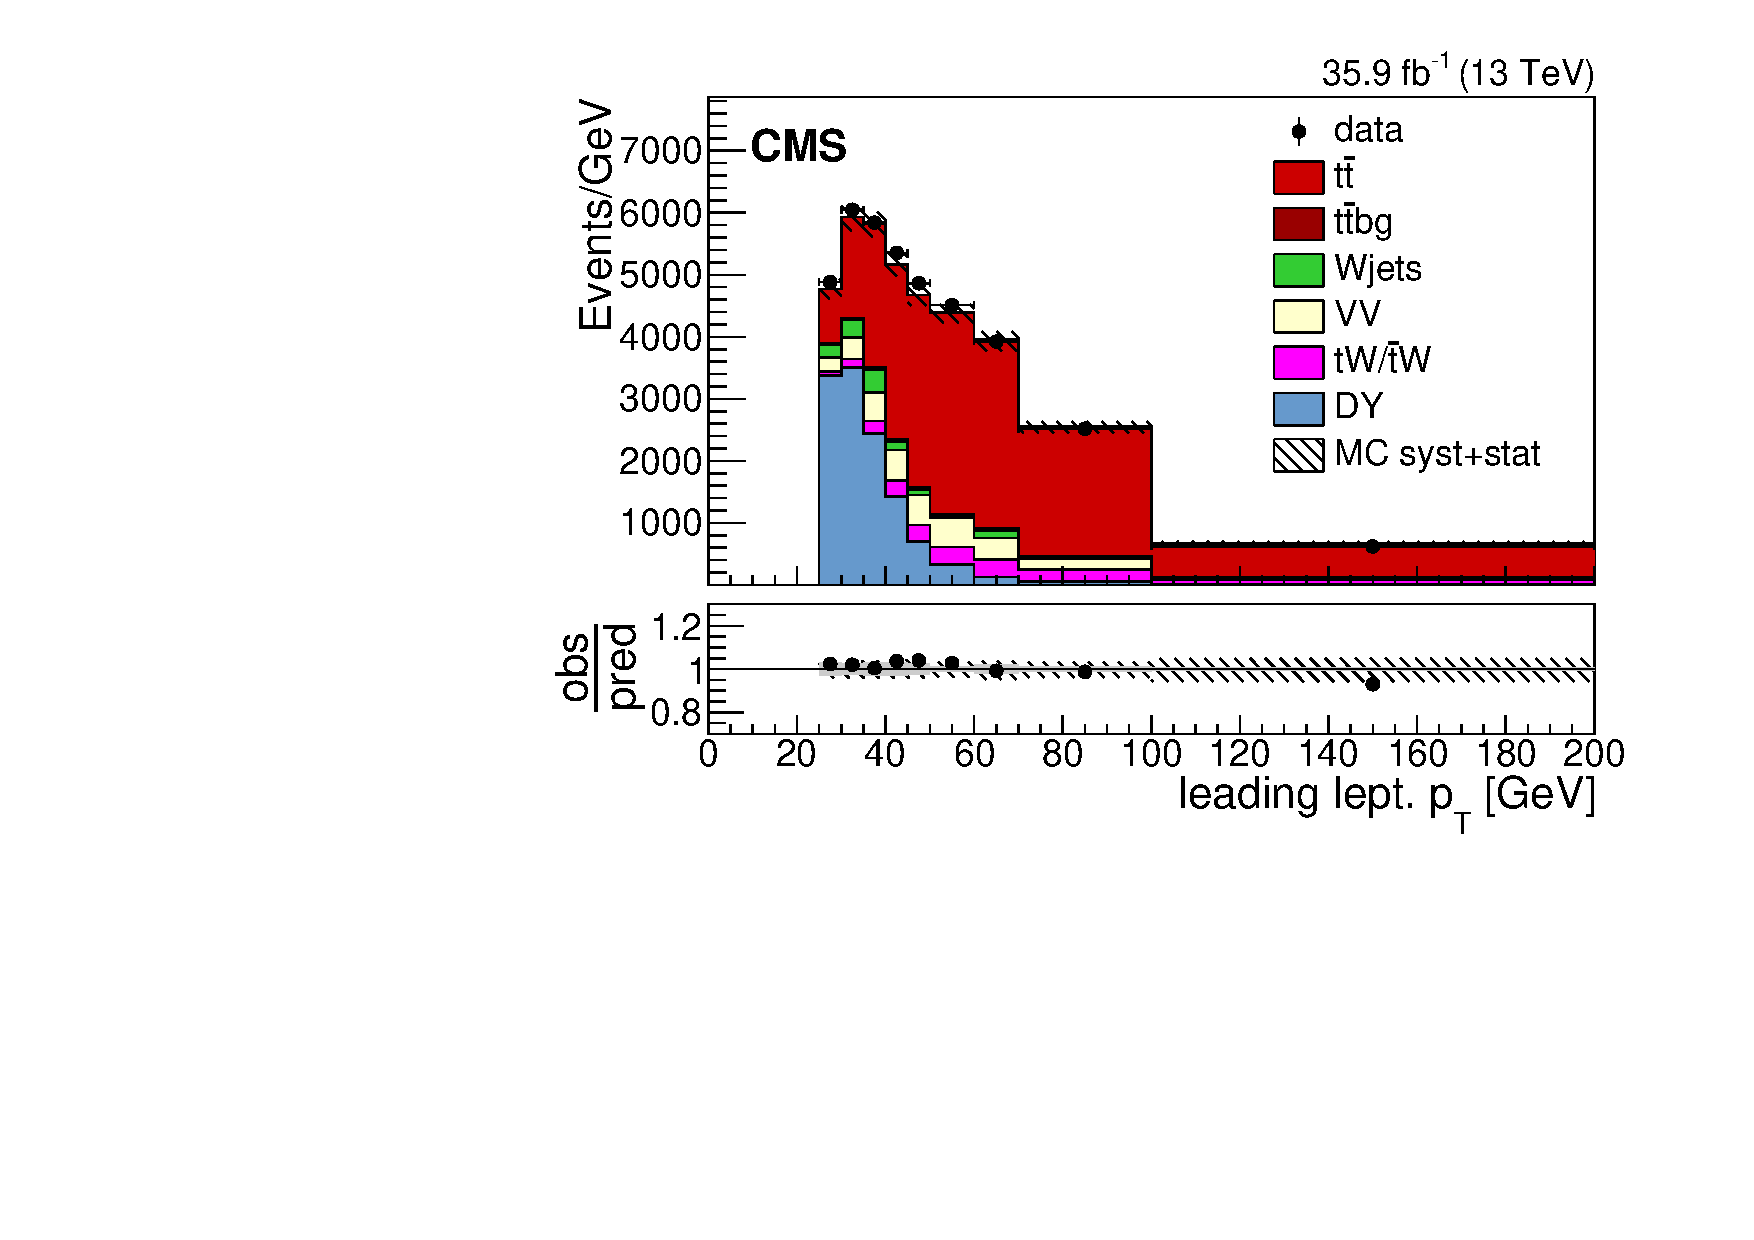
\includegraphics{CrossSection/Figures/ControlPlots/emu_sysnom/lead_lepton_pt_step_8.pdf}}
    \resizebox{0.48 \textwidth}{!}{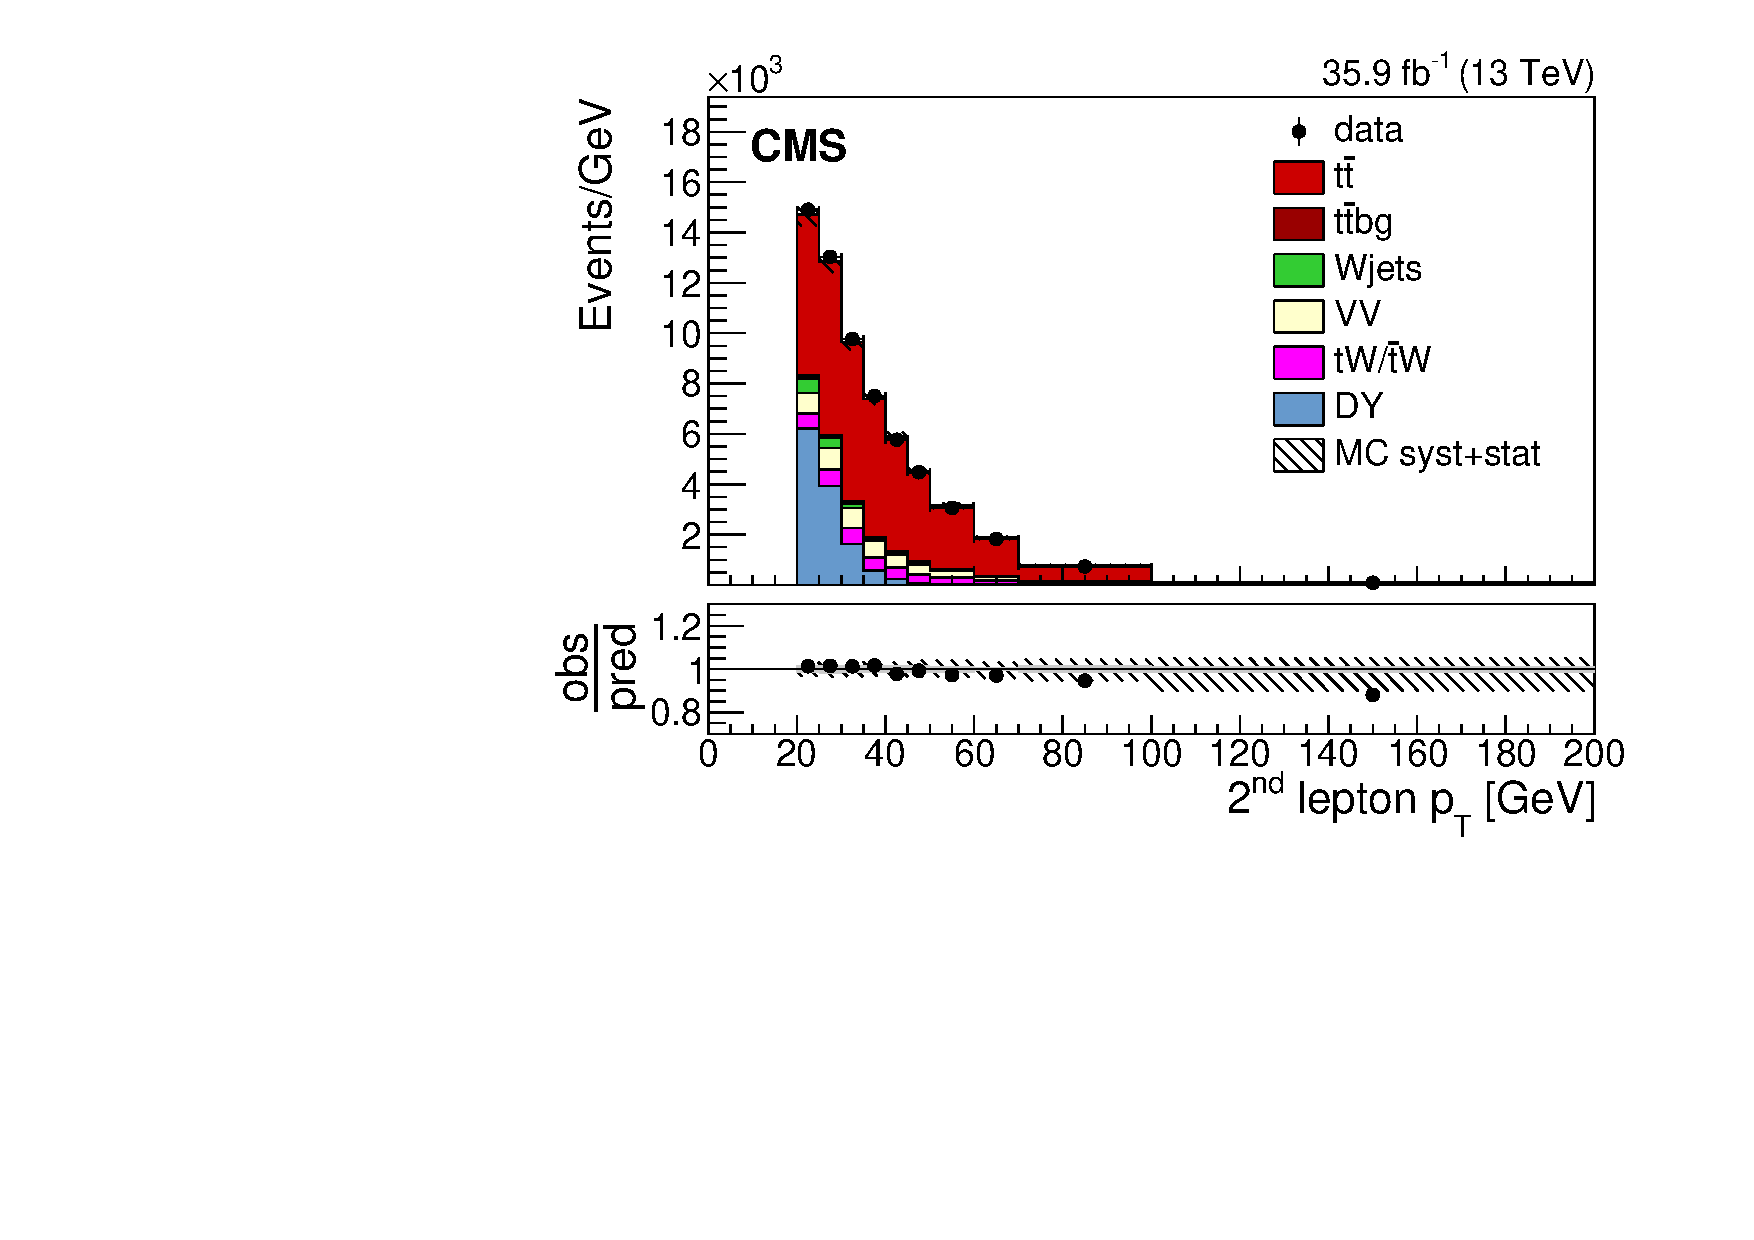
\includegraphics{CrossSection/Figures/ControlPlots/emu_sysnom/seclead_lepton_pt_step_8.pdf}}
        \resizebox{0.48 \textwidth}{!}{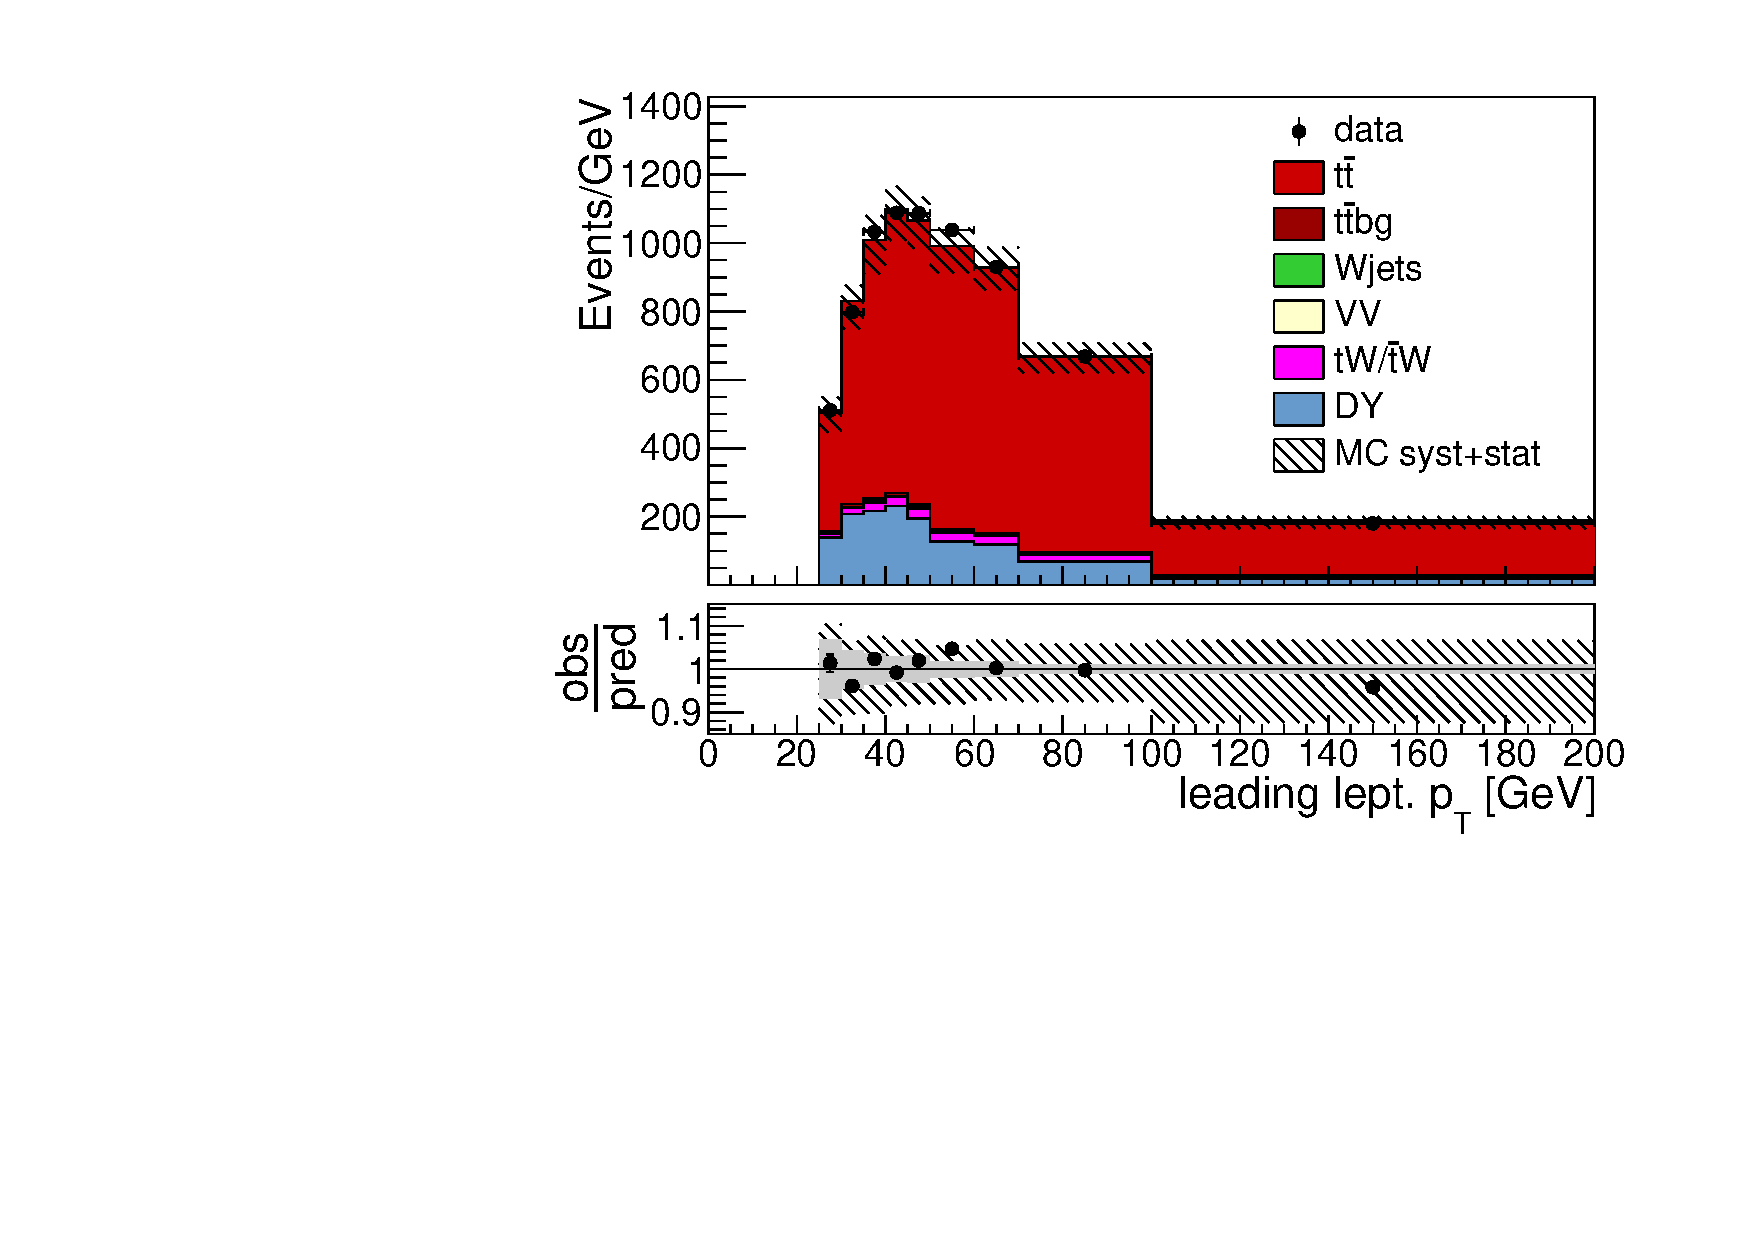
\includegraphics{CrossSection/Figures/ControlPlots/mumu_sysnom/lead_lepton_pt_step_8.pdf}}
    \resizebox{0.48 \textwidth}{!}{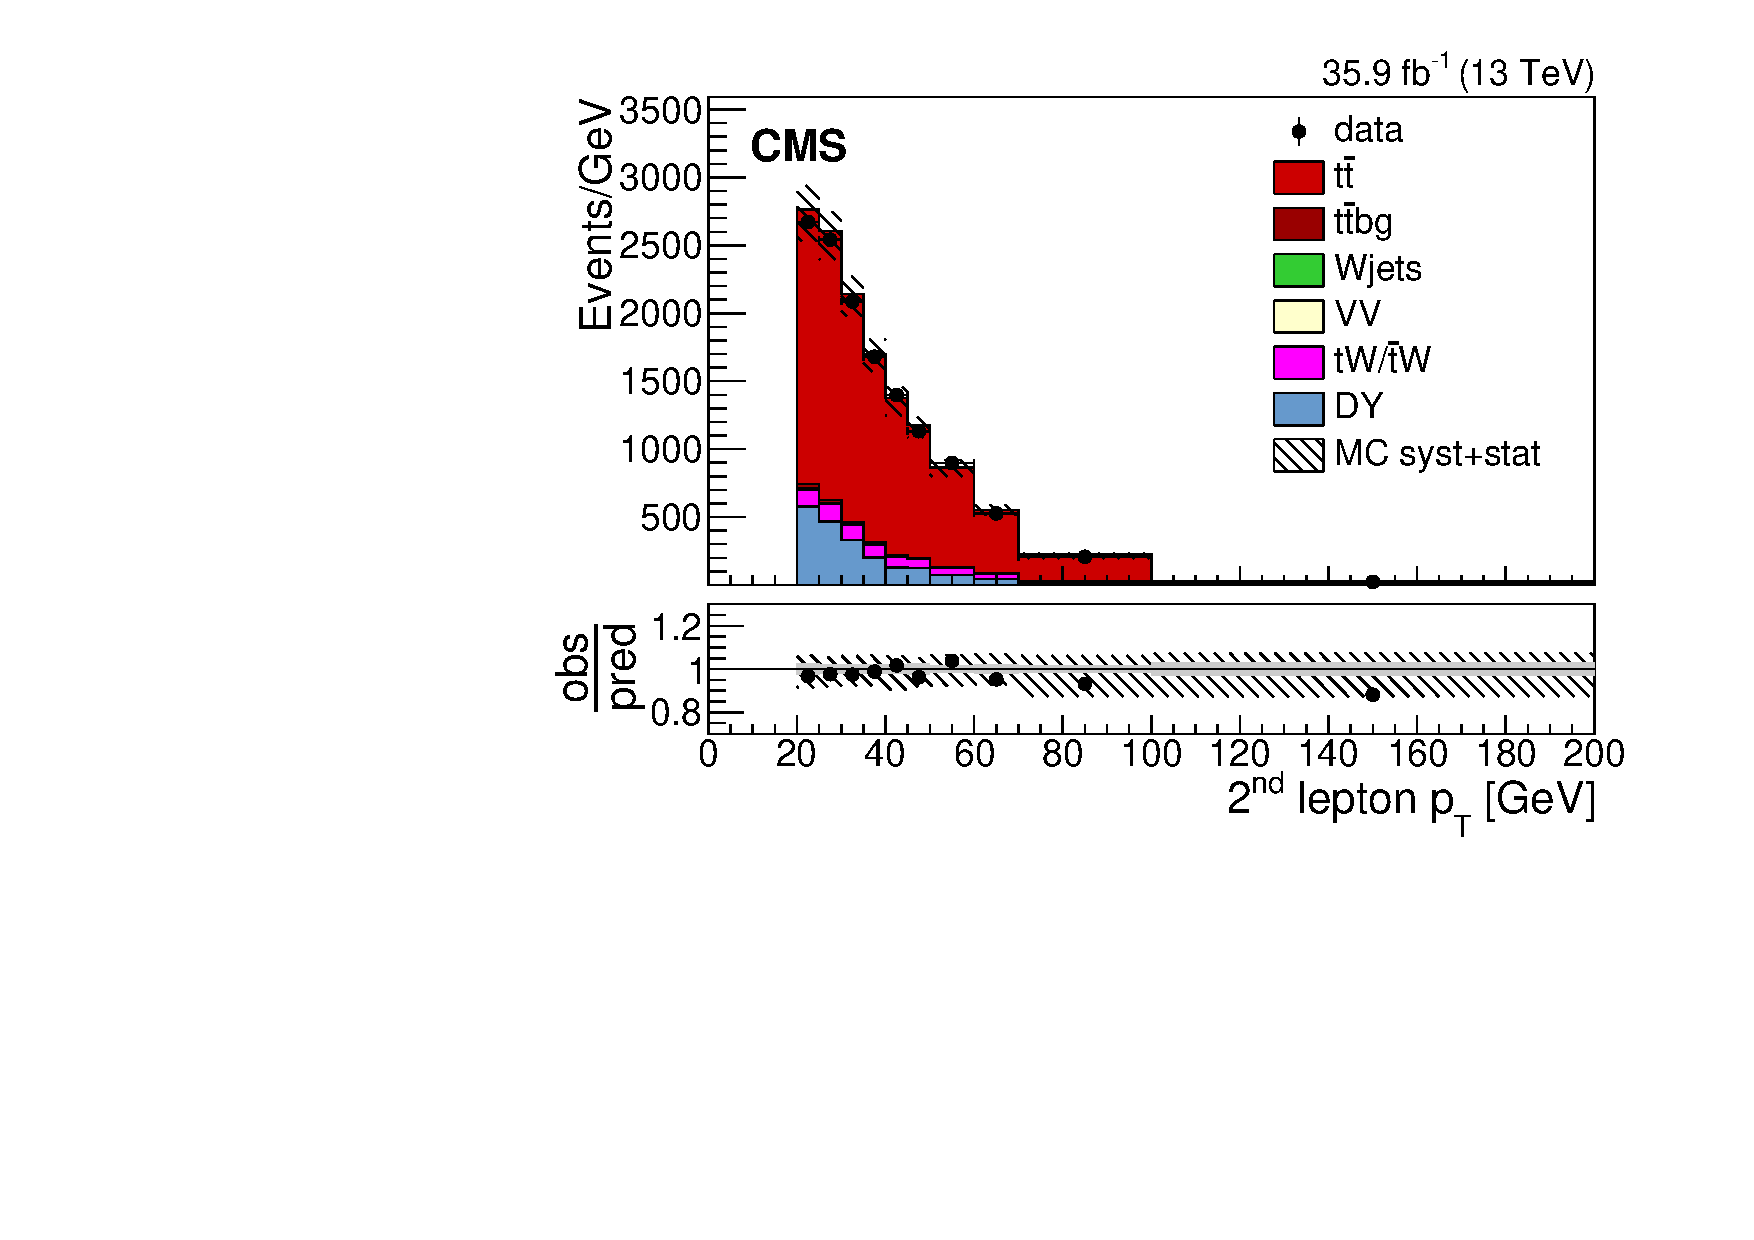
\includegraphics{CrossSection/Figures/ControlPlots/mumu_sysnom/seclead_lepton_pt_step_8.pdf}}
    \resizebox{0.48 \textwidth}{!}{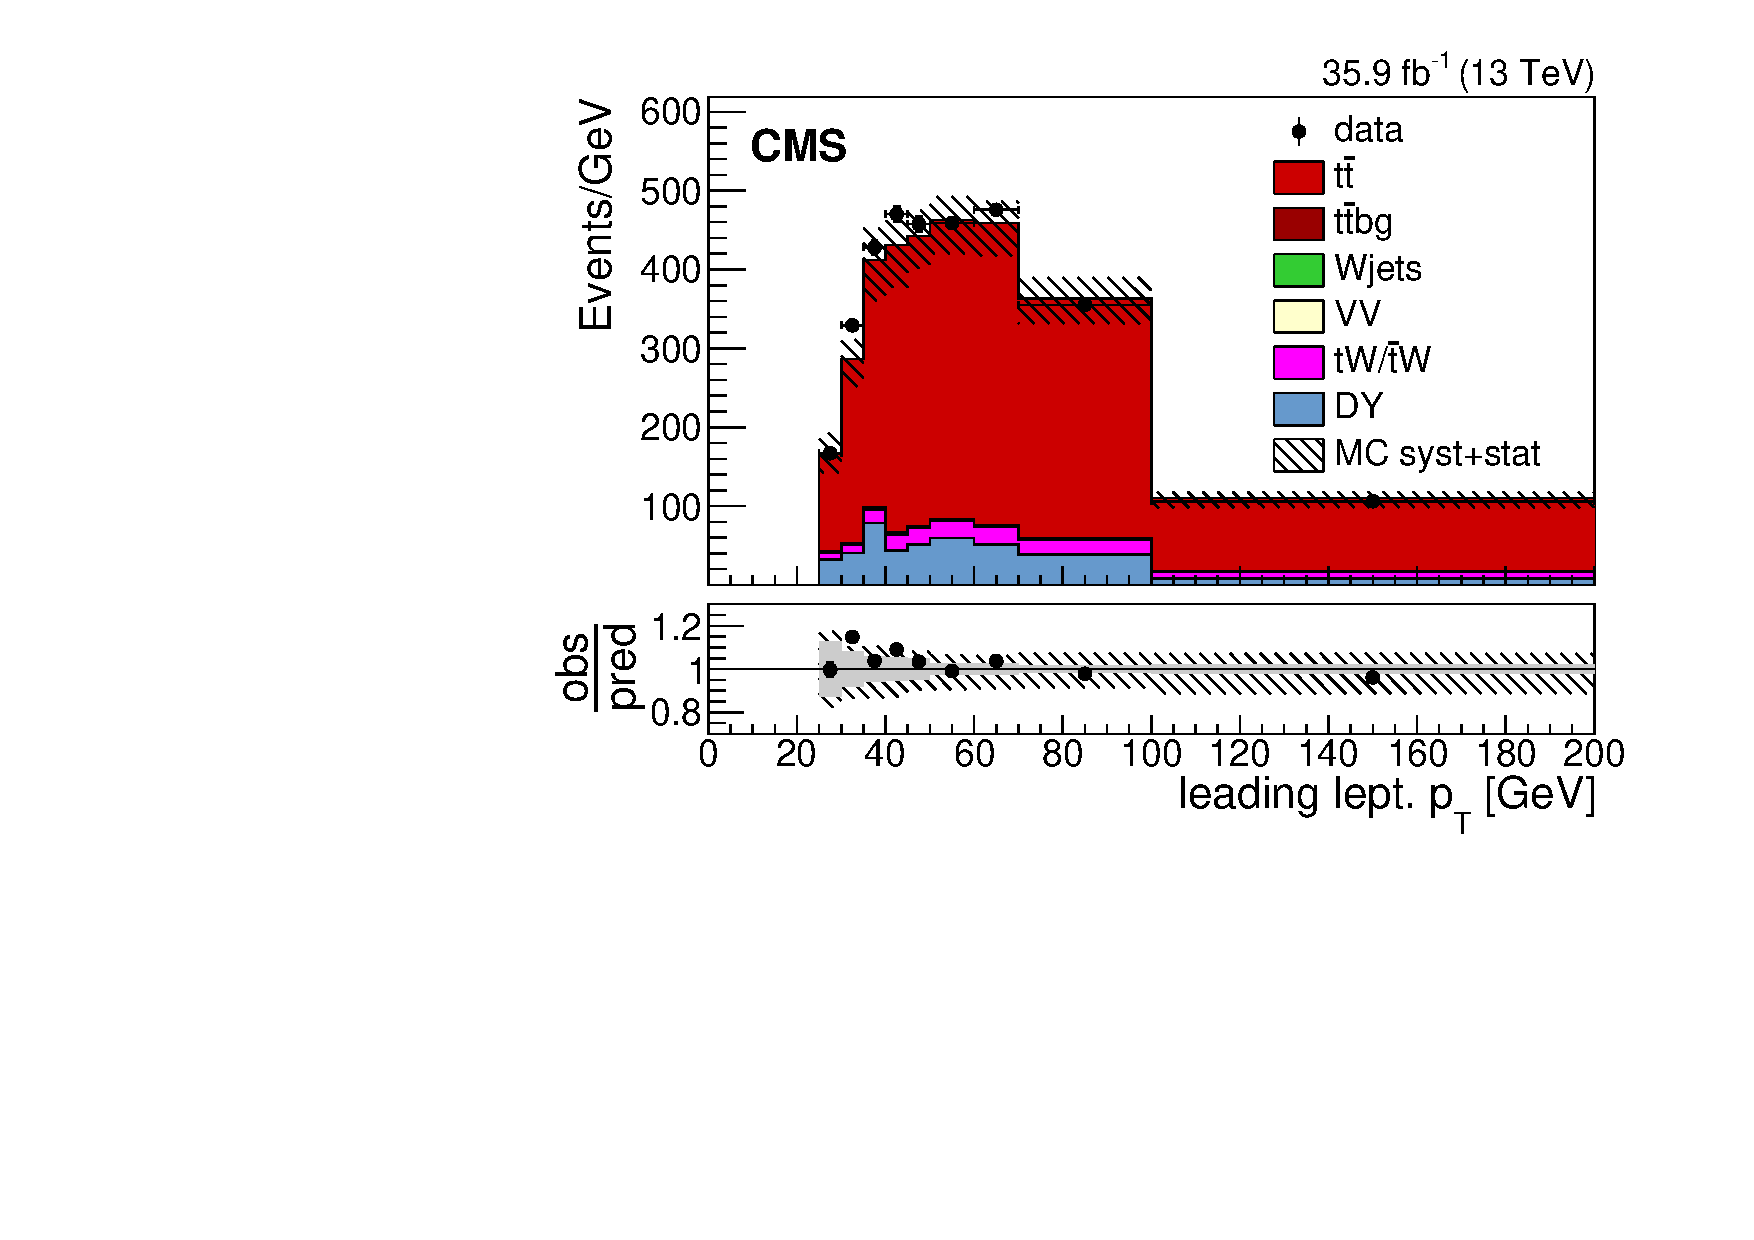
\includegraphics{CrossSection/Figures/ControlPlots/ee_sysnom/lead_lepton_pt_step_8.pdf}}
    \resizebox{0.48 \textwidth}{!}{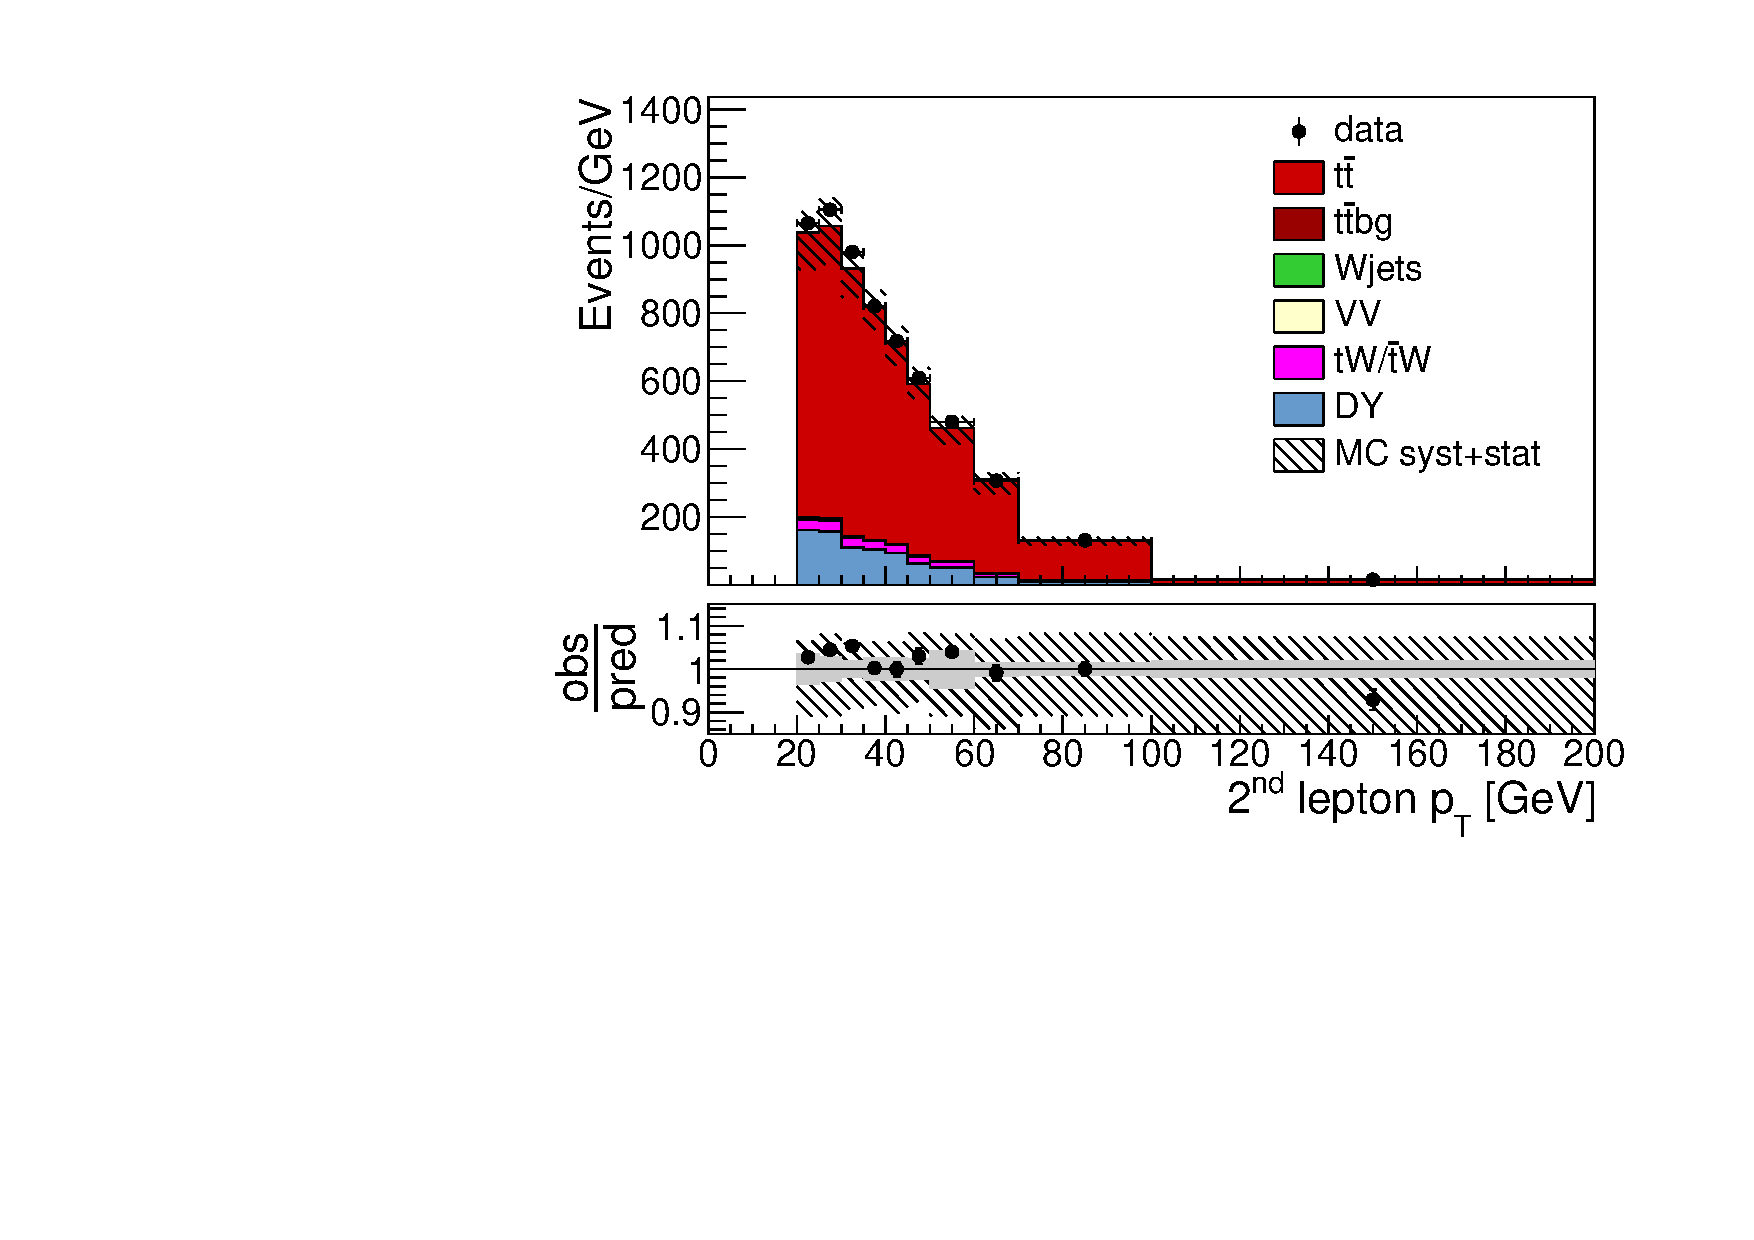
\includegraphics{CrossSection/Figures/ControlPlots/ee_sysnom/seclead_lepton_pt_step_8.pdf}}
      \caption{Transverse momentum of the leading(left) and trailing (right)
        lepton in the \emu (upper row), \mumu (middle row) and \ee (lower row) decay channels.
        The events are shown after the
        event selection.  The hatched
        bands correspond to the total uncertainty on the sum of the
        predicted yields. 
        %agrohsje , excluding luminosity and background
        %normalization uncertainties. 
        The ratios of data to the sum of the predicted yields are
        shown at the bottom pannel of each plot. The solid gray band
        represents the contribution of the statistical uncertainty.}  
       \label{fig:xsec_pt_ctrplots}
  \end{center}
\end{figure}

The $\eta$ for the leading and trailing lepton for all three decay channels is shown in Figure \ref{fig:xsec_eta_ctrplots}.
The plots show that both leptons tend to be found in the central region of the detector for \ttbar events.
For electrons (\emu and \ee chanel) the $\eta$ distribution shows a gap around $|\eta| \approx 1.5$. This reduction in the number of events is caused by a instrumentation gap in the ECAL (see Section \ref{sec:xsec_sel})
Otherwise the $\eta$ distribution is smooth as seen for the \mumu channel.
The simulation generally predicts the measurement within the uncertainties. The systematic uncertainties are generally higher for larger $\eta$ values, as uncertainties on the lepton reconstruction
tend to increase if the lepton is detected int he endcaps of the detector.


\begin{figure}[htbp!]
  \begin{center}
    \resizebox{0.48 \textwidth}{!}{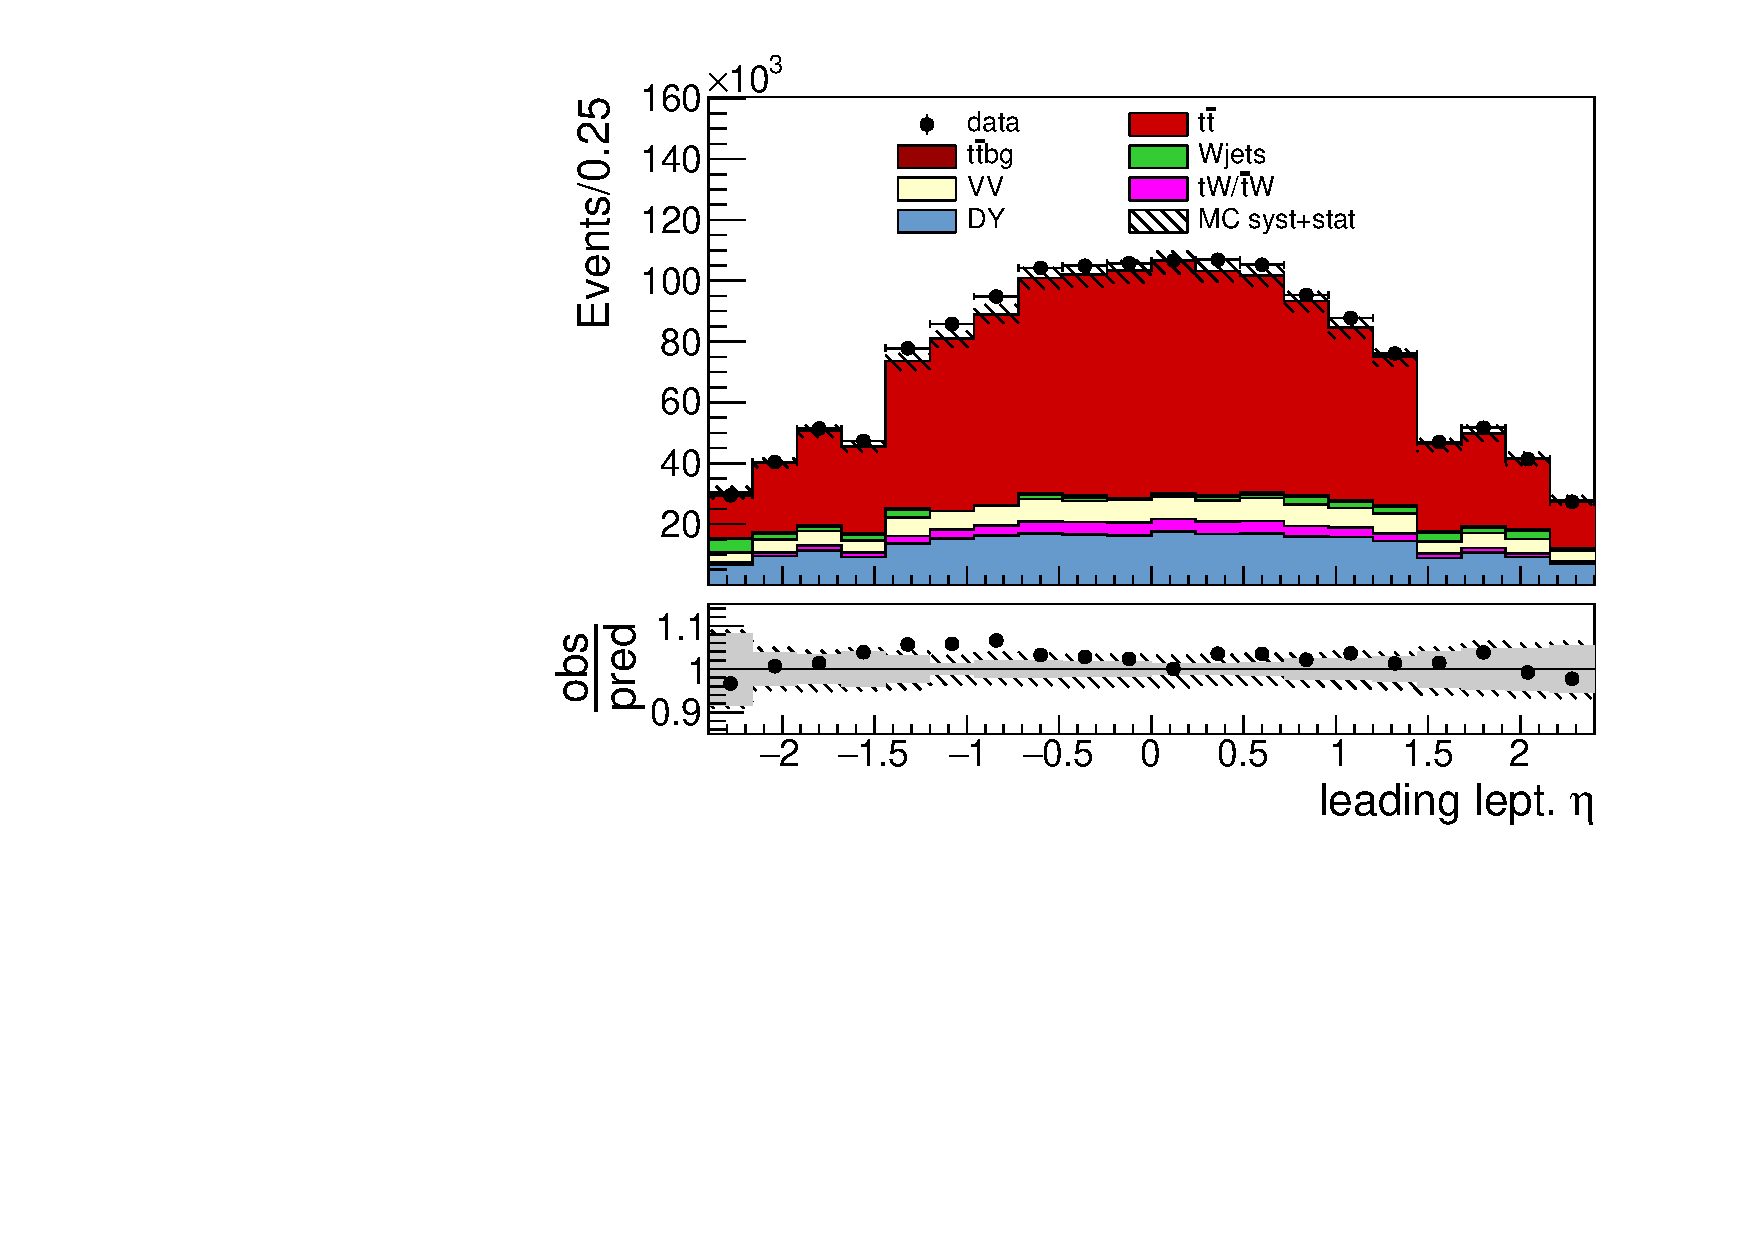
\includegraphics{CrossSection/Figures/ControlPlots/emu_sysnom/lead_lepton_eta_step_8.pdf}}
    \resizebox{0.48 \textwidth}{!}{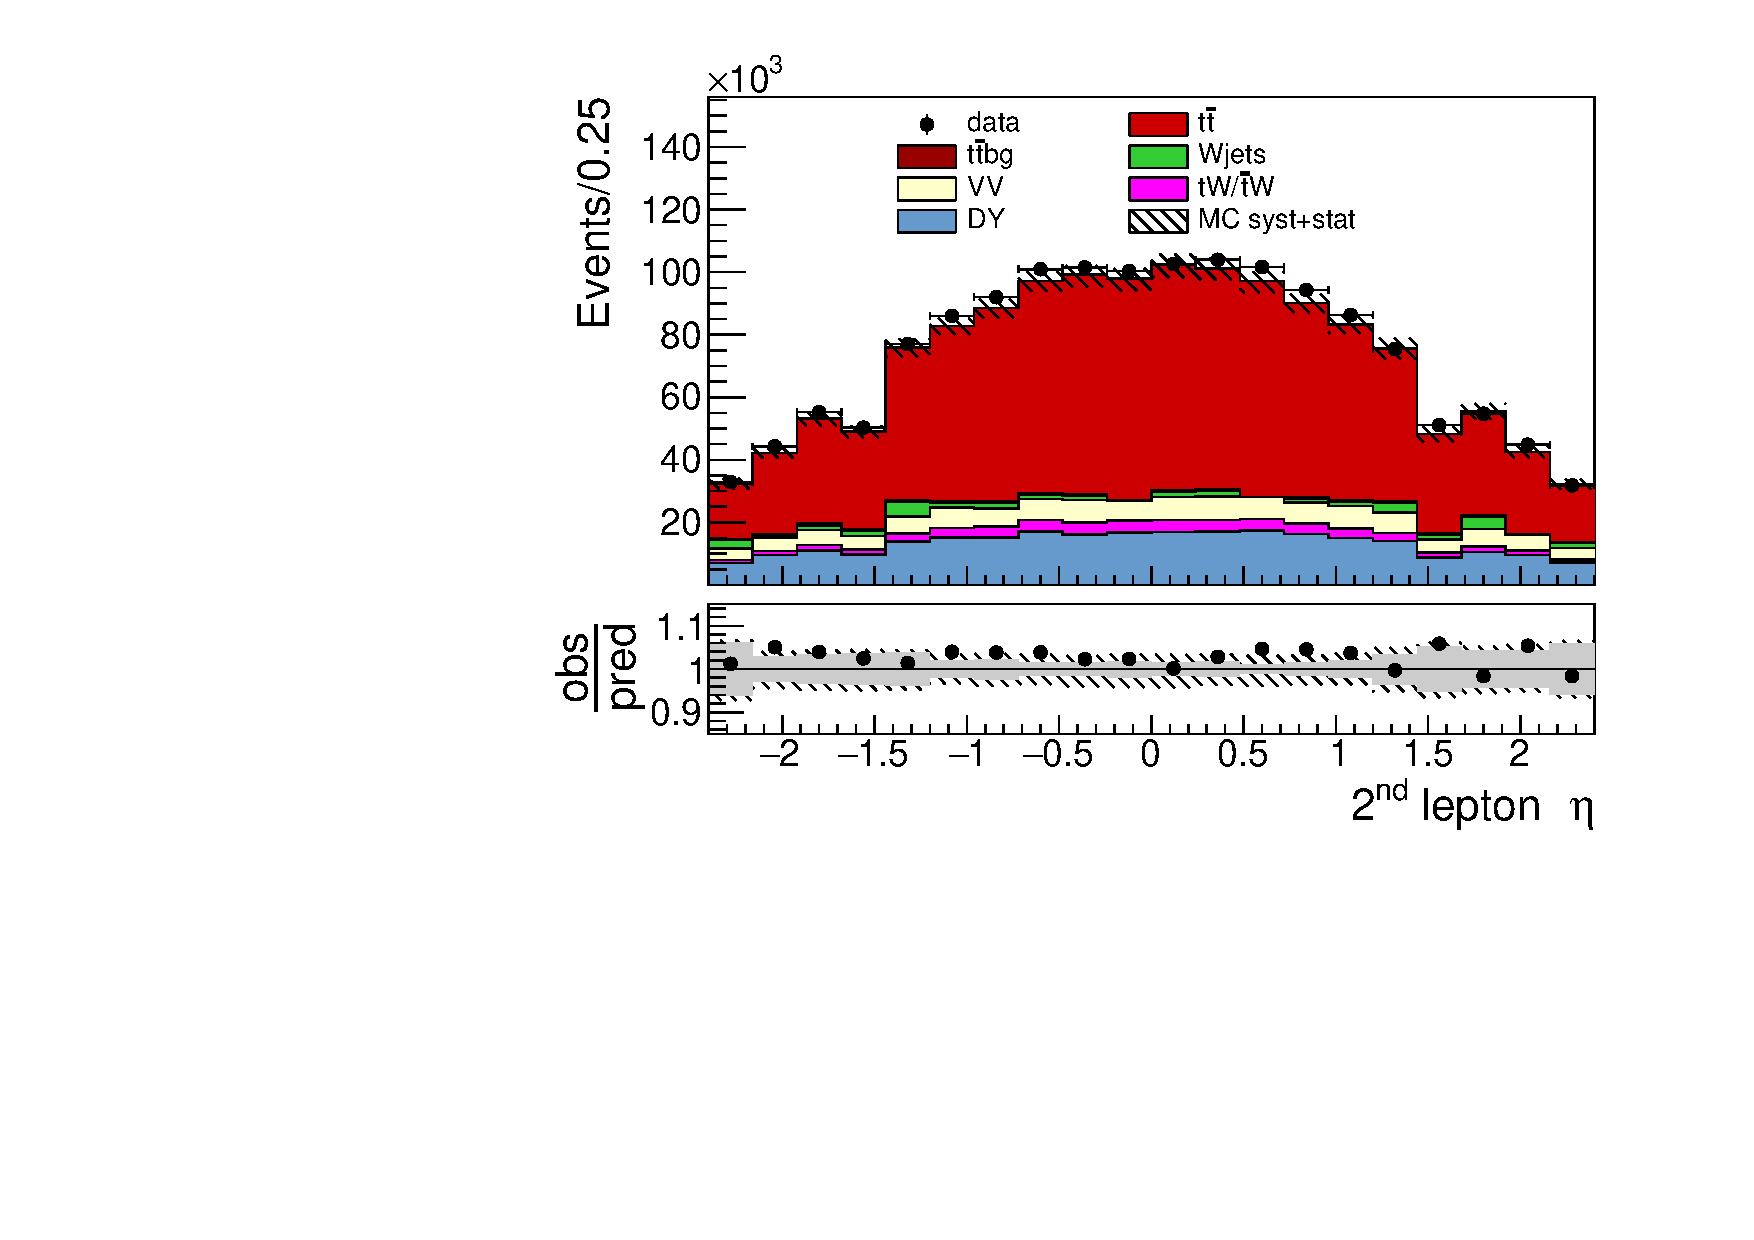
\includegraphics{CrossSection/Figures/ControlPlots/emu_sysnom/seclead_lepton_eta_step_8.pdf}}
        \resizebox{0.48 \textwidth}{!}{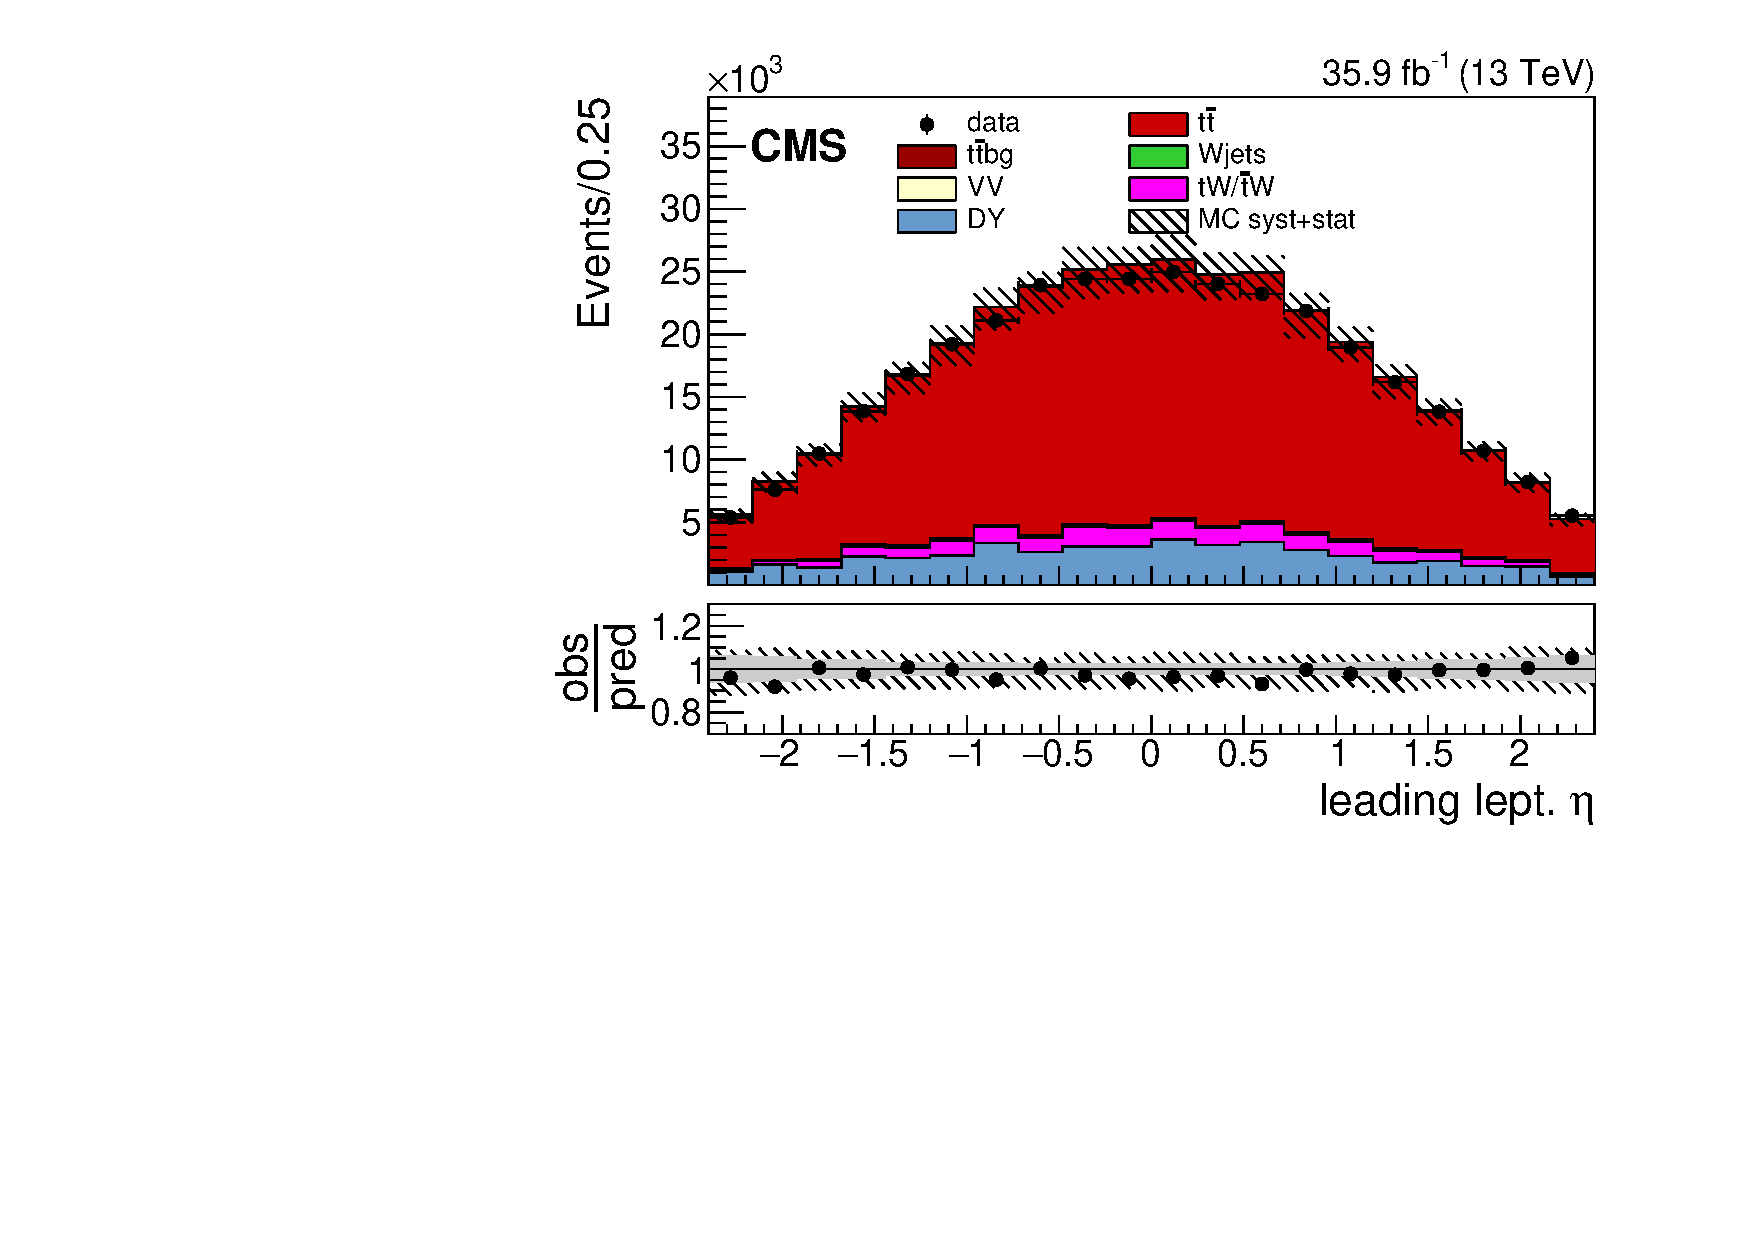
\includegraphics{CrossSection/Figures/ControlPlots/mumu_sysnom/lead_lepton_eta_step_8.pdf}}
    \resizebox{0.48 \textwidth}{!}{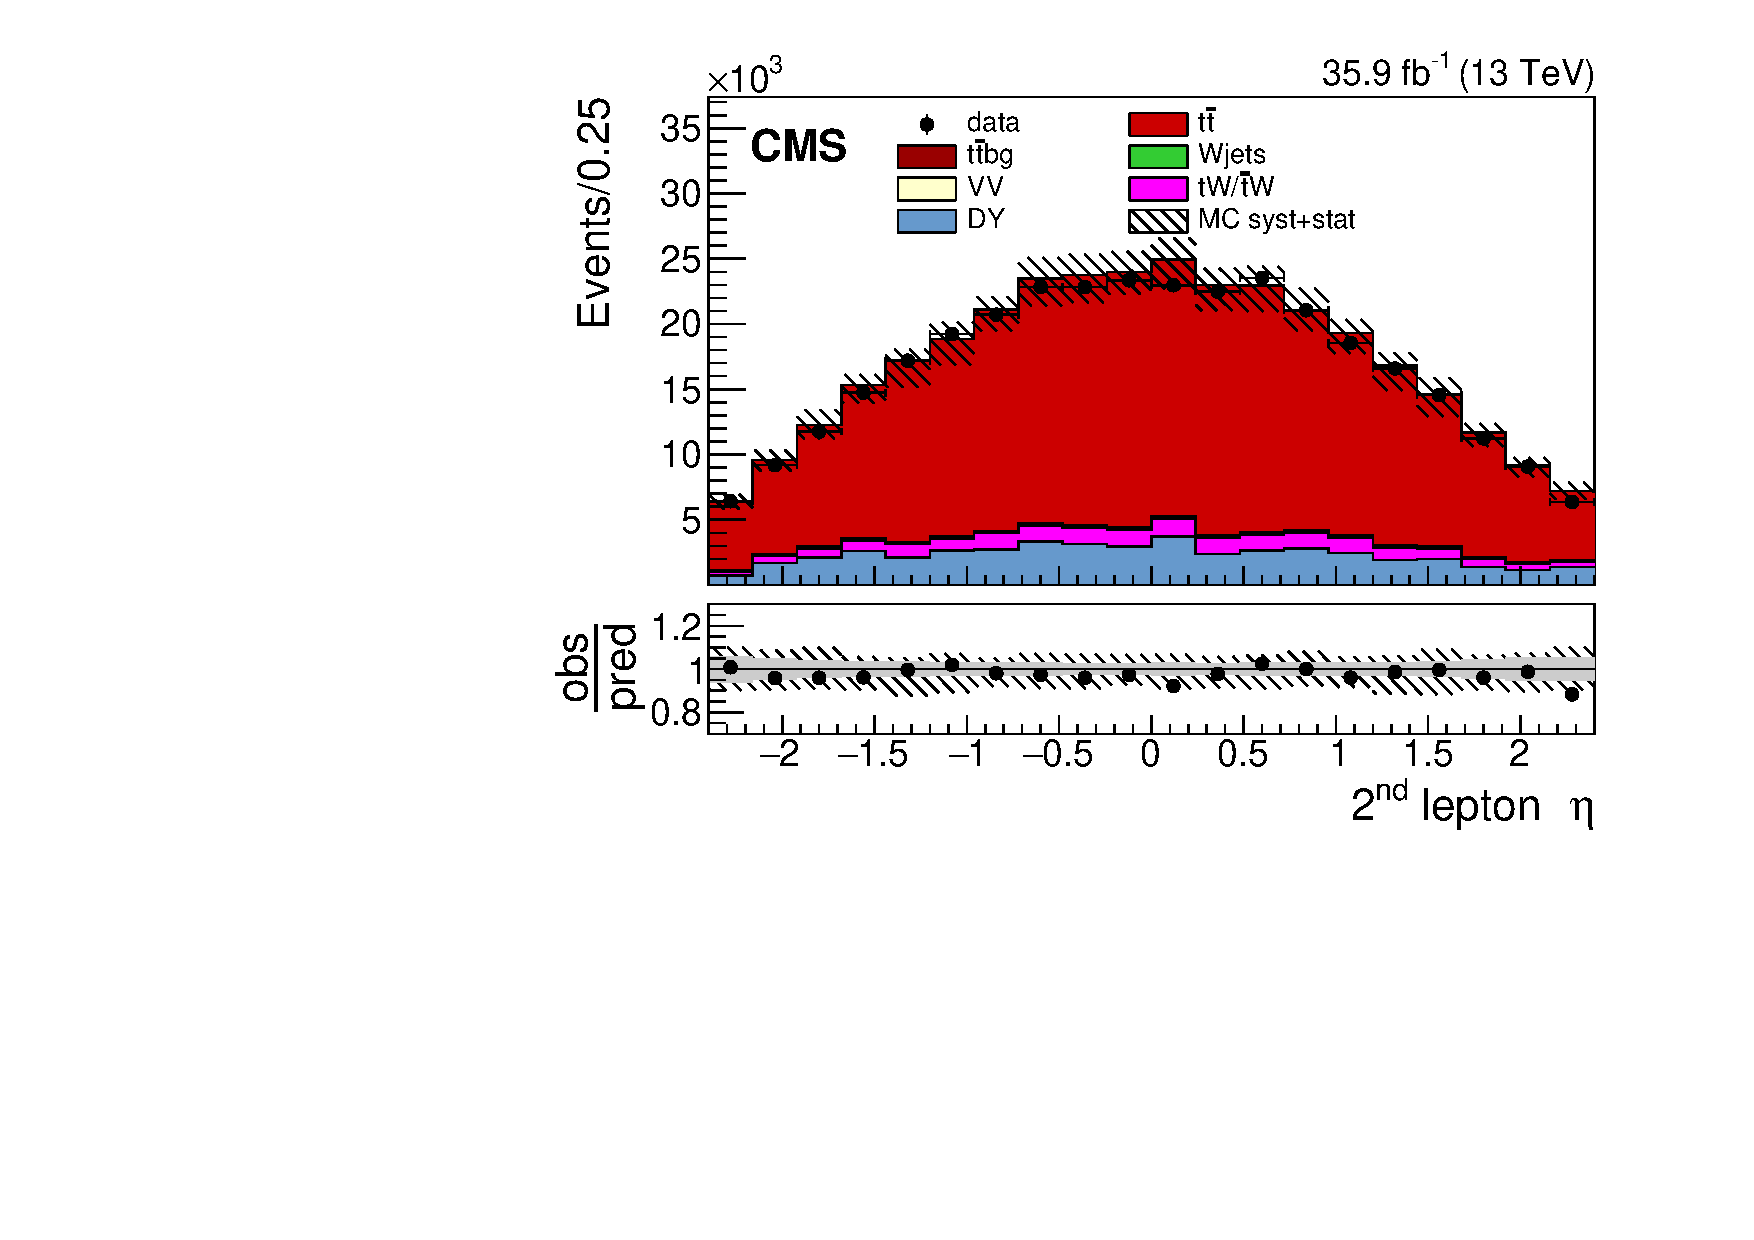
\includegraphics{CrossSection/Figures/ControlPlots/mumu_sysnom/seclead_lepton_eta_step_8.pdf}}
    \resizebox{0.48 \textwidth}{!}{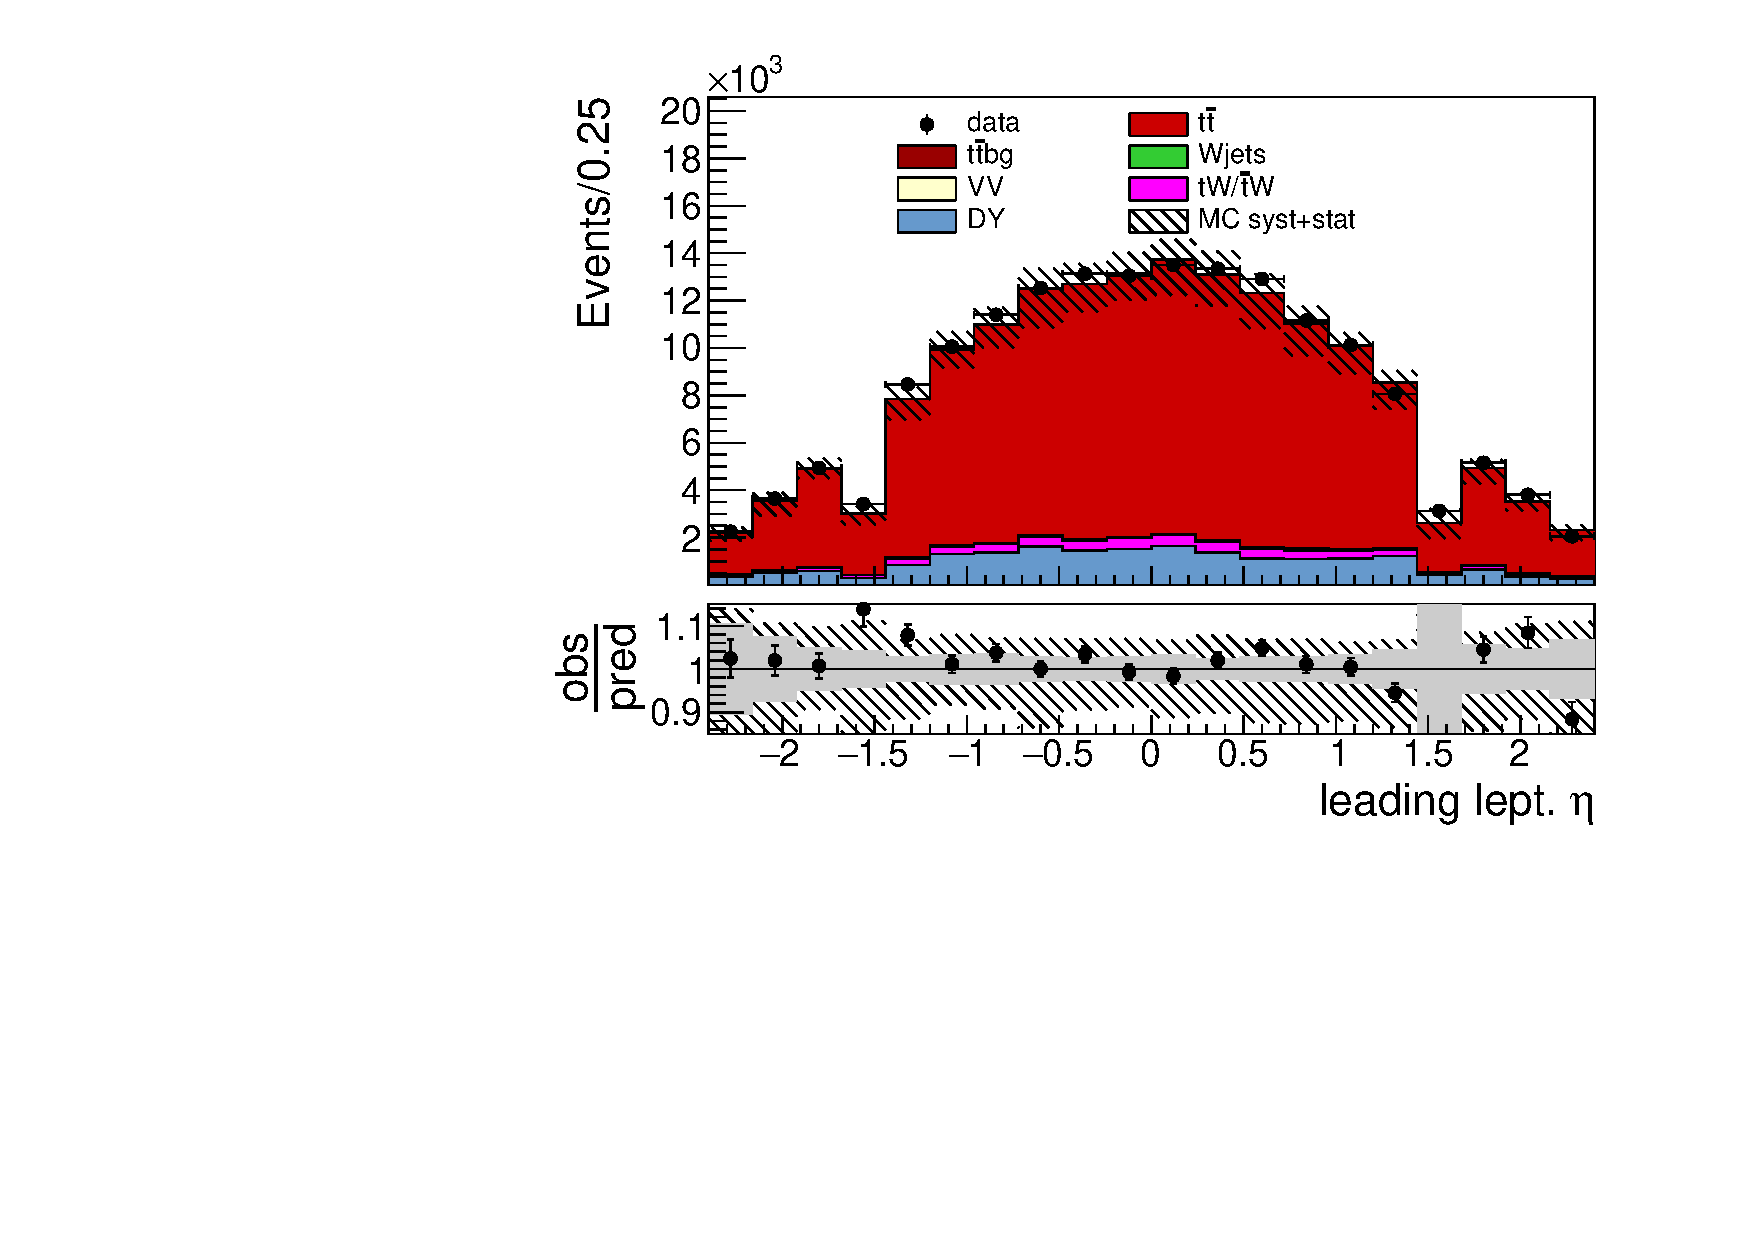
\includegraphics{CrossSection/Figures/ControlPlots/ee_sysnom/lead_lepton_eta_step_8.pdf}}
    \resizebox{0.48 \textwidth}{!}{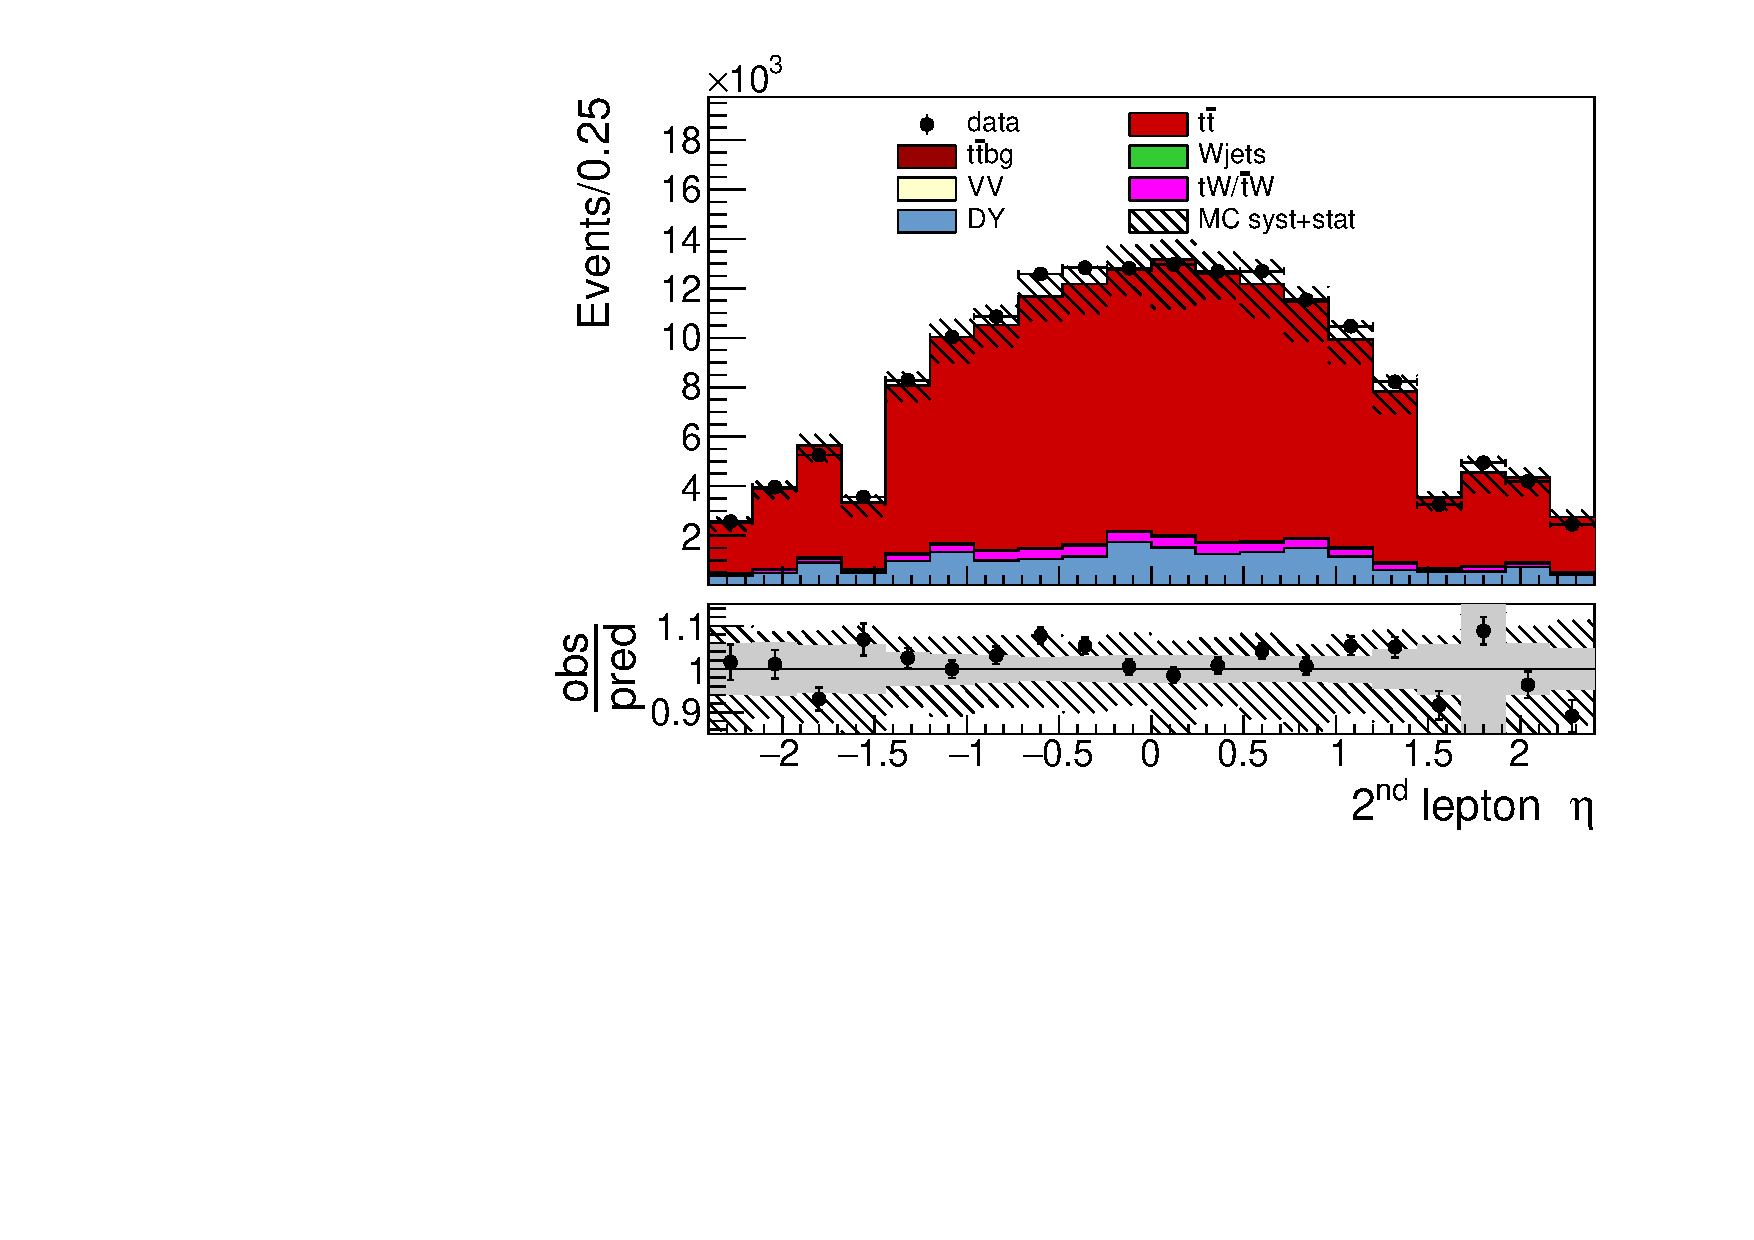
\includegraphics{CrossSection/Figures/ControlPlots/ee_sysnom/seclead_lepton_eta_step_8.pdf}}
      \caption{Pseudo rapidity for the leading(left) and trailing (right)
        lepton in the \emu (upper row), \mumu (middle row) and \ee (lower row) decay channels.
        The events are shown after the
        event selection.  The hatched
        bands correspond to the total uncertainty on the sum of the
        predicted yields. 
        %agrohsje , excluding luminosity and background
        %normalization uncertainties. 
        The ratios of data to the sum of the predicted yields are
        shown at the bottom pannel of each plot. The solid gray band
        represents the contribution of the statistical uncertainty.}  
       \label{fig:xsec_eta_ctrplots}
  \end{center}
\end{figure}



The number of jets for all three channels is shown on Figure \ref{fig:xsec_jets_ctrplots}.
The largest contribution from \ttbar events can be found in the bin for exactly two jets. 
Events with zero jets are cut for the \ee and \mumu channel are cut, but the \emu channel shows that the signal
contribution in that region of phase space is comparitevly small.
As seen in all channels \ttbar signal events tend to contain more jets compared to the background events, as two jets come from the top decays and initial gluons can be radiated from both the initial state and the top quarks themselves. 
Radiation of additional gluons is only possible for the initial state quarks in Drell-Yan events.

The prediction and the measurement do not agree for a high number of jets in the \emu and \mumu channels.
In the specific simulation used here \ref{sec:SimReco_Sim} up to 3 jets are simulated in the hard process, while any additional jets are produced in the parton shower.
The more extreme ranges of the phase space, such as events with more than five additional jets are not neccesarily perfectly simulated.
This is a well known issue in the simulation of \ttbar events and as shown in the figures its well covered by the systematic variations. Especially the systematic variations for the parton shower parameters chosen for the simulation
(see Section \ref{sec:theo_uncert}) contribute in that region of phase space.
In the \ee channel the statistical uncertainty on both the measurement and the prediction is to large to draw a decisive conclusion.

\begin{figure}[htbp!]
  \begin{center}
    \resizebox{0.48 \textwidth}{!}{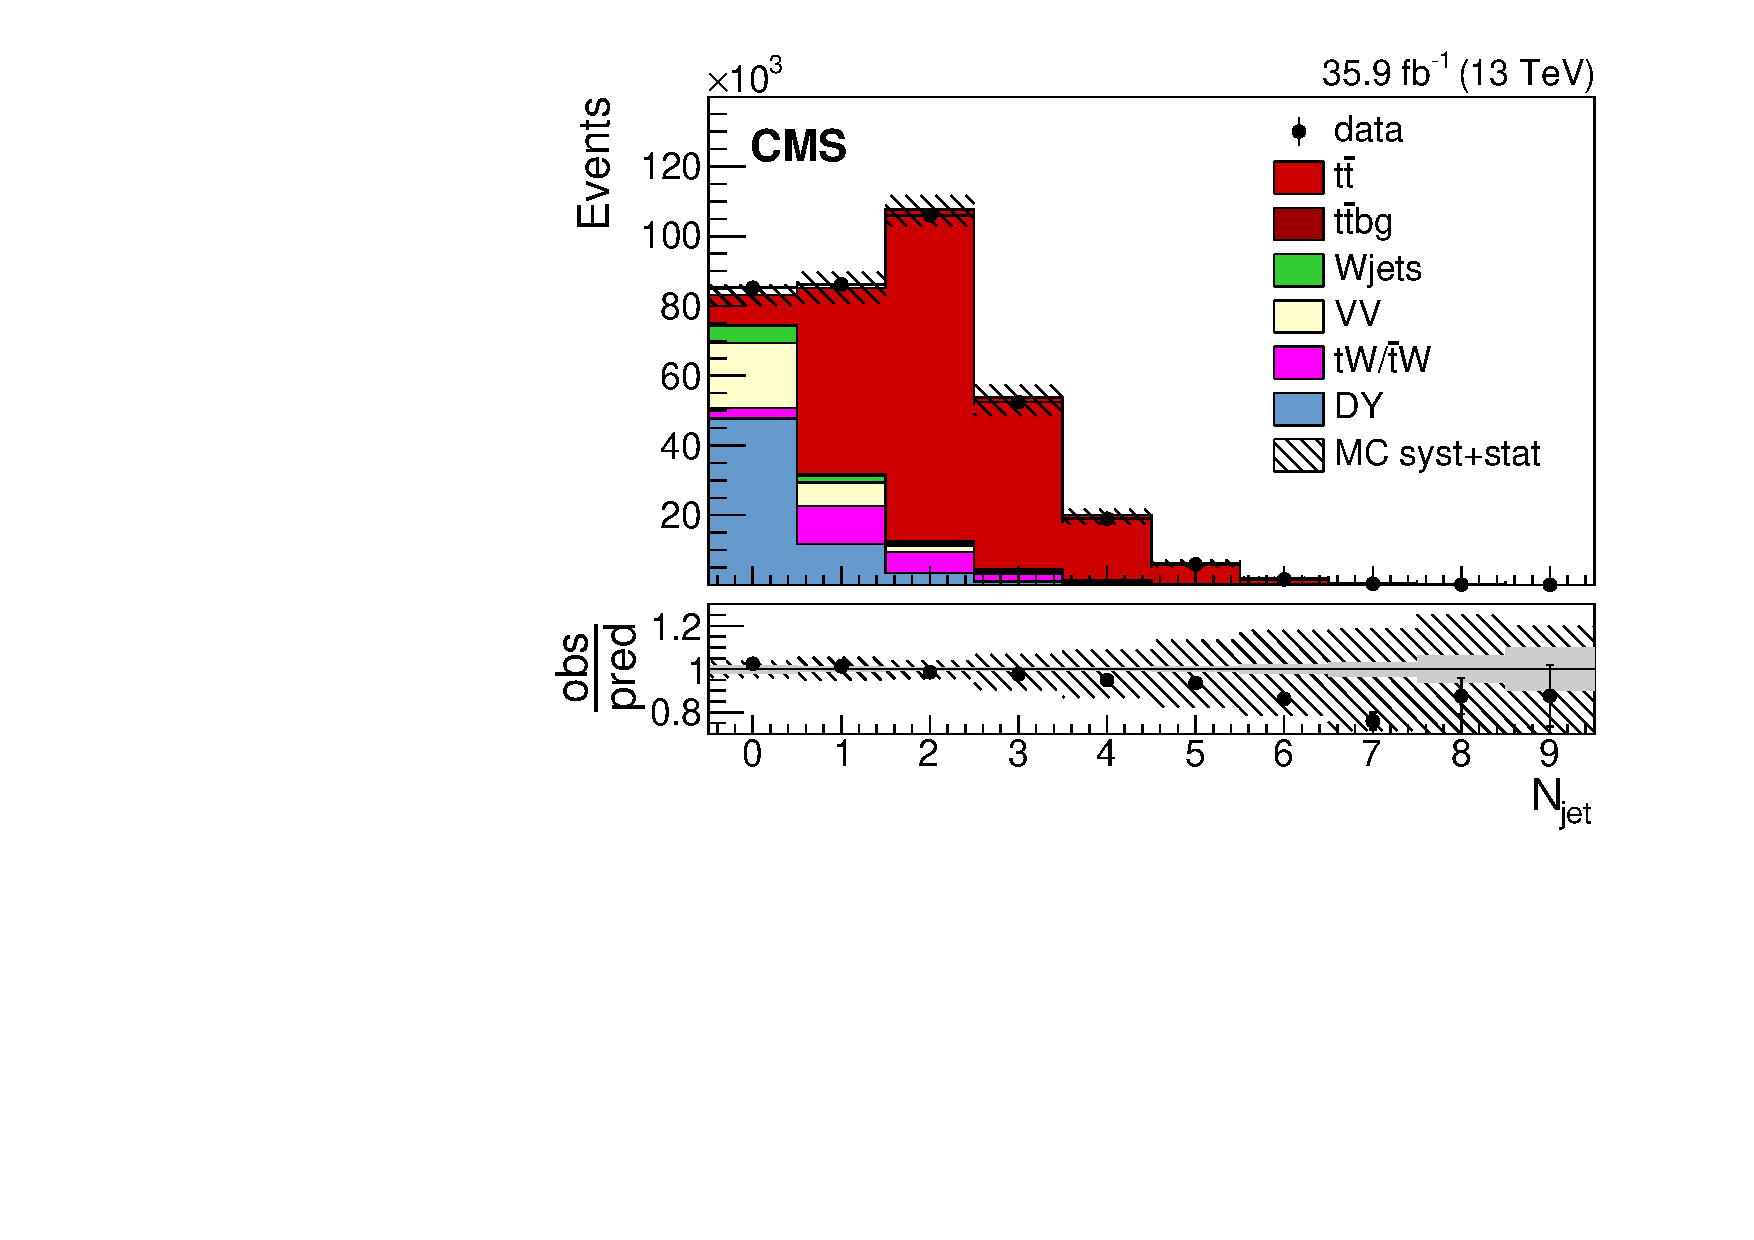
\includegraphics{CrossSection/Figures/ControlPlots/emu_sysnom/selected_jets_multi_step_8.pdf}}
    \resizebox{0.48 \textwidth}{!}{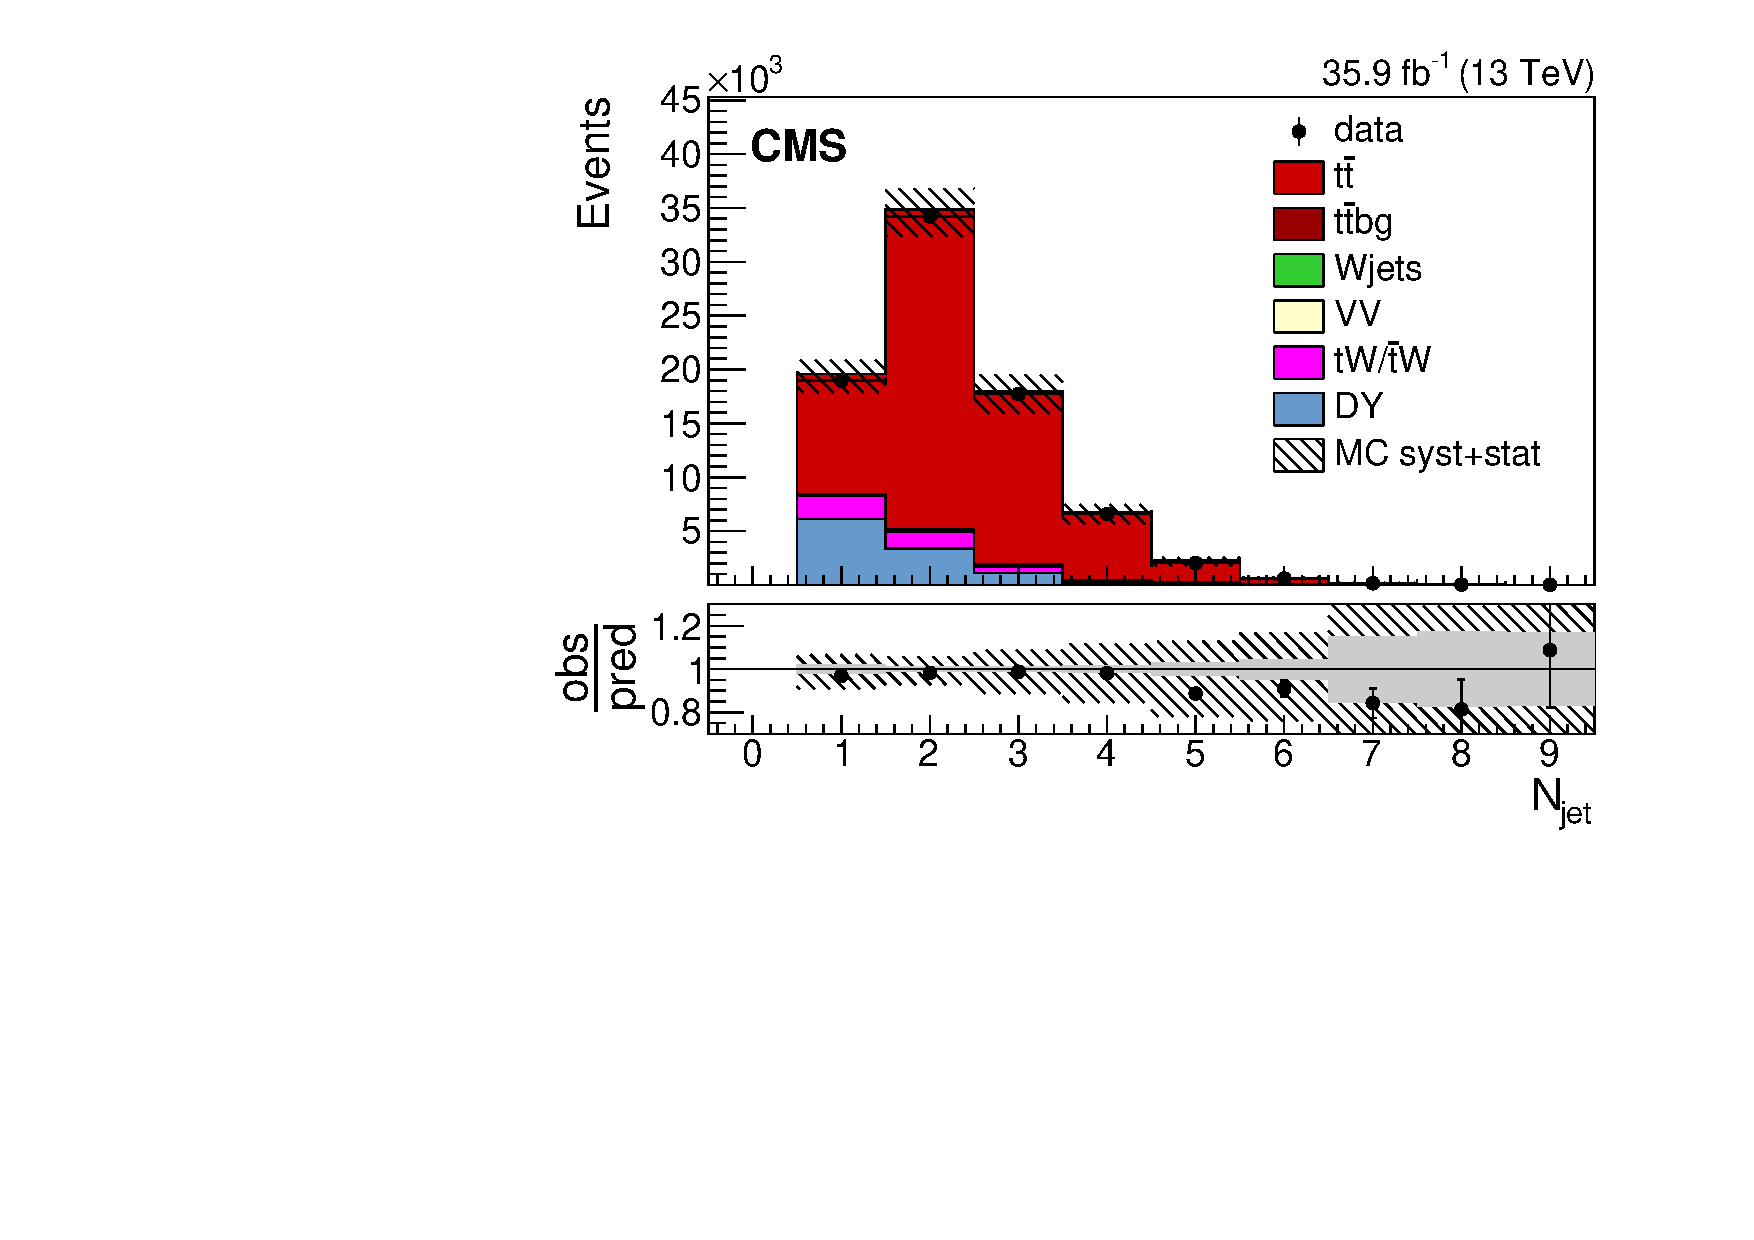
\includegraphics{CrossSection/Figures/ControlPlots/mumu_sysnom/selected_jets_multi_step_8.pdf}}
    \resizebox{0.48 \textwidth}{!}{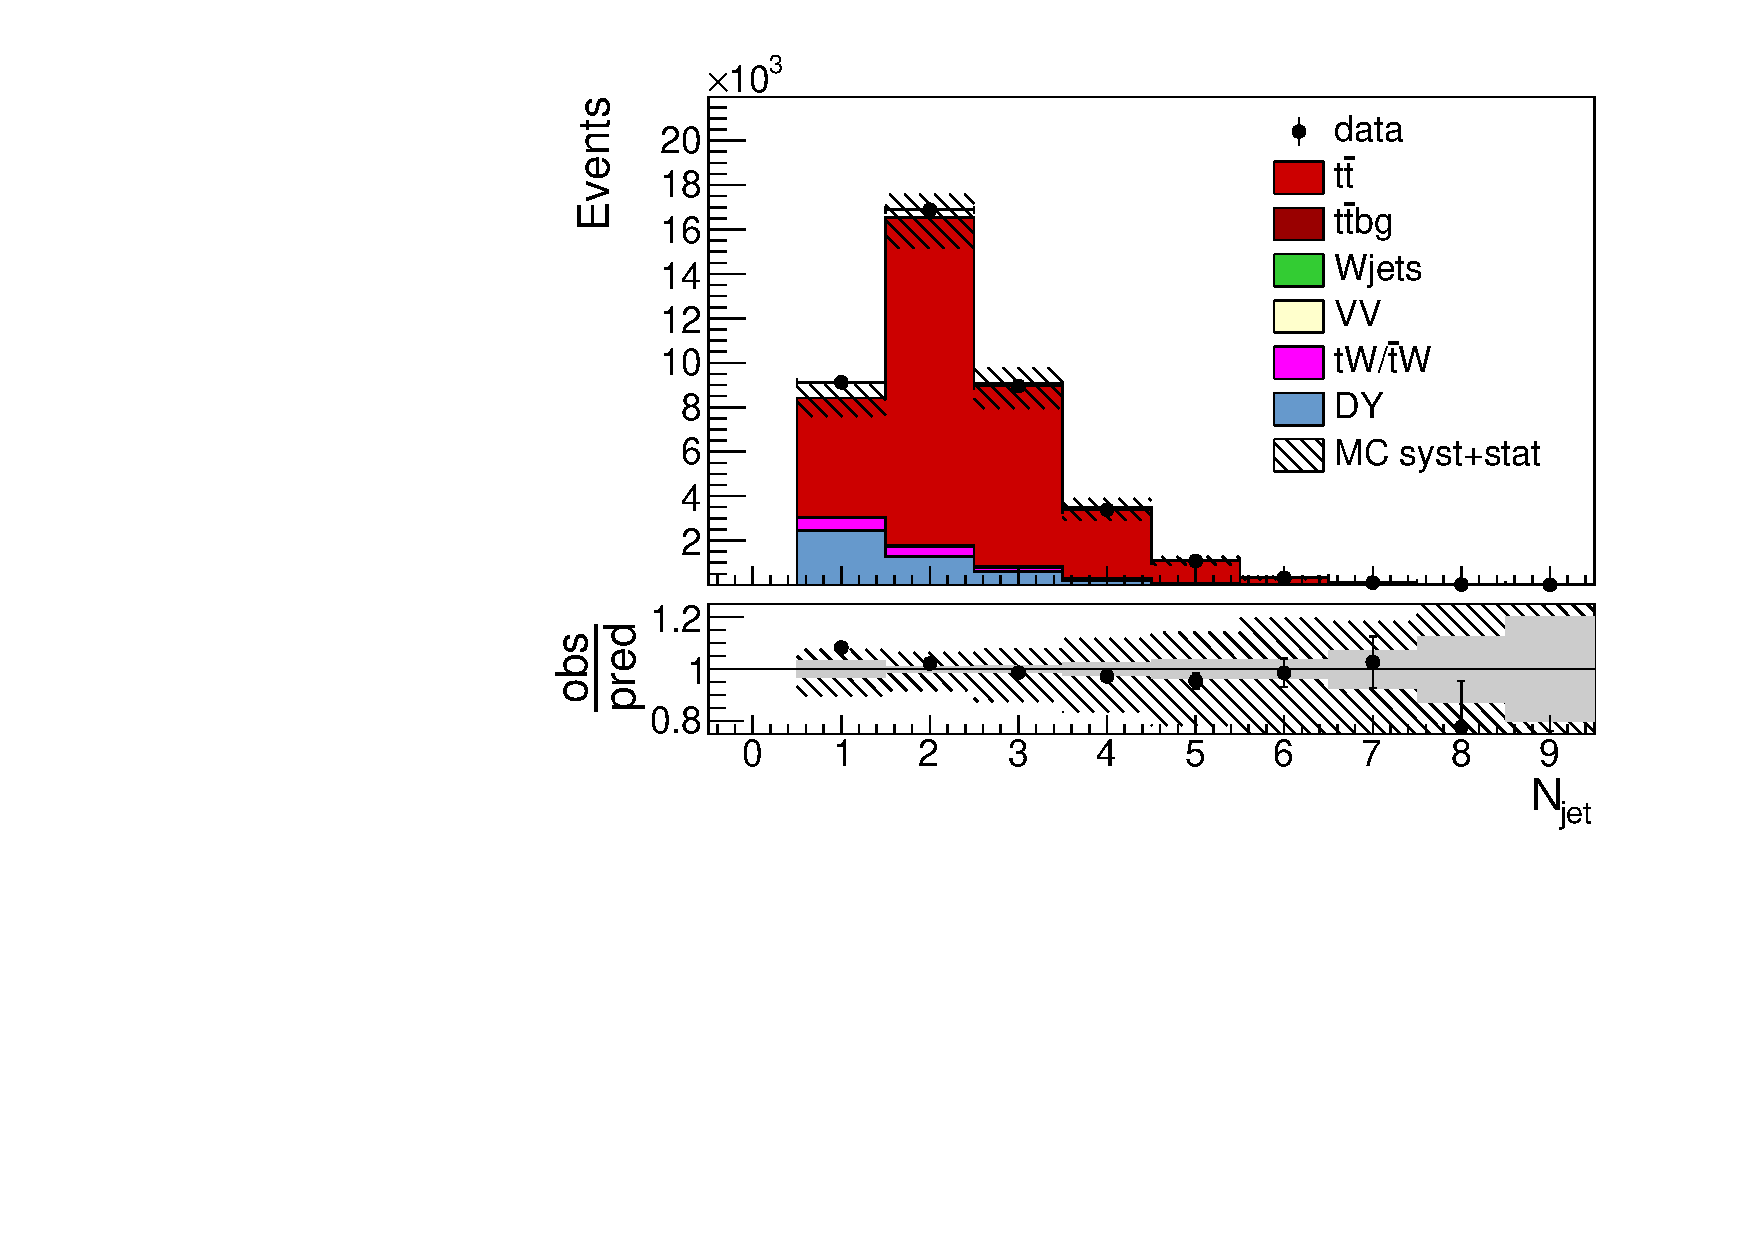
\includegraphics{CrossSection/Figures/ControlPlots/ee_sysnom/selected_jets_multi_step_8.pdf}}
    \caption{Number of jets \emu (upper left), \mumu (upper right) and \ee (lower row) decay channels.
        The events are shown after the
        event selection.  The hatched
        bands correspond to the total uncertainty on the sum of the
        predicted yields. 
        %agrohsje , excluding luminosity and background
        %normalization uncertainties. 
        The ratios of data to the sum of the predicted yields are
        shown at the bottom pannel of each plot. The solid gray band
        represents the contribution of the statistical uncertainty.}  
       \label{fig:xsec_jets_ctrplots}
  \end{center}
\end{figure}

The number of b tagged jets for all three channels is shown in Figure \ref{fig:xsec_bjets_ctrplots}.
Events with zero b tagged jets are cut for the same flavor channels.
A considerable amount of \ttbar signal events contain zero b tagged jets, due to the comparatively low efficiency to identify a jet containing a b quark.
However, the low amoung of background events containing one or more b-tagged jet shows the low probatibility to wrongly identify a jet as b tagged.
The main remaining background contribution with one or more b tagged jet in the \emu channel are single top events, which contain a b quark from the top quark decay.
In the same flavor channel Drell-Yan events contribute as well.
The simulation reproduces the behaviour in data in all three channels.

As shown in the plots variables relating to (b tagged) jets provide discrimination between signal and background. This separation power makes these variables good candidates to 
further separate signal and background in the subsequent steps of the analysis.

\begin{figure}[htbp!]
  \begin{center}
    \resizebox{0.48 \textwidth}{!}{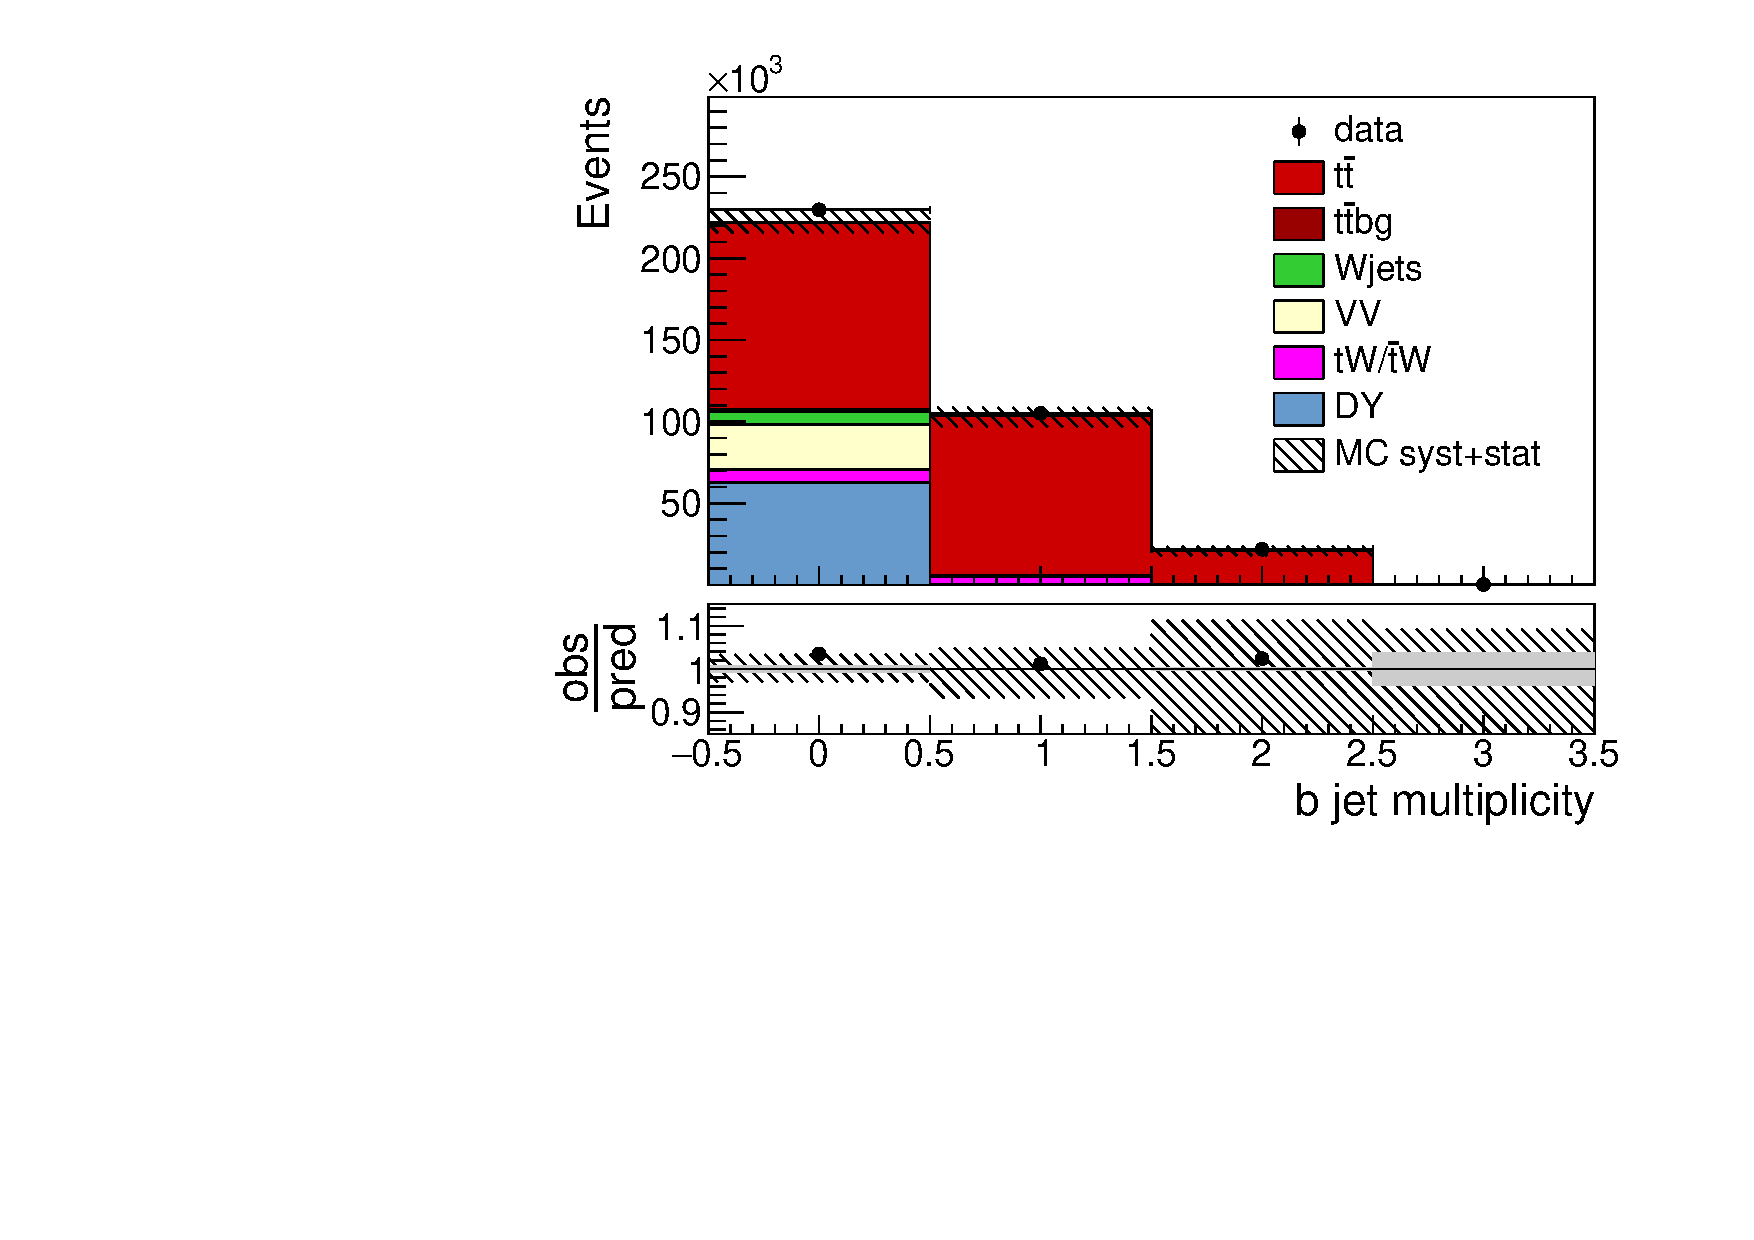
\includegraphics{CrossSection/Figures/ControlPlots/emu_sysnom/selected_b-jet_multi_step_8.pdf}}
    \resizebox{0.48 \textwidth}{!}{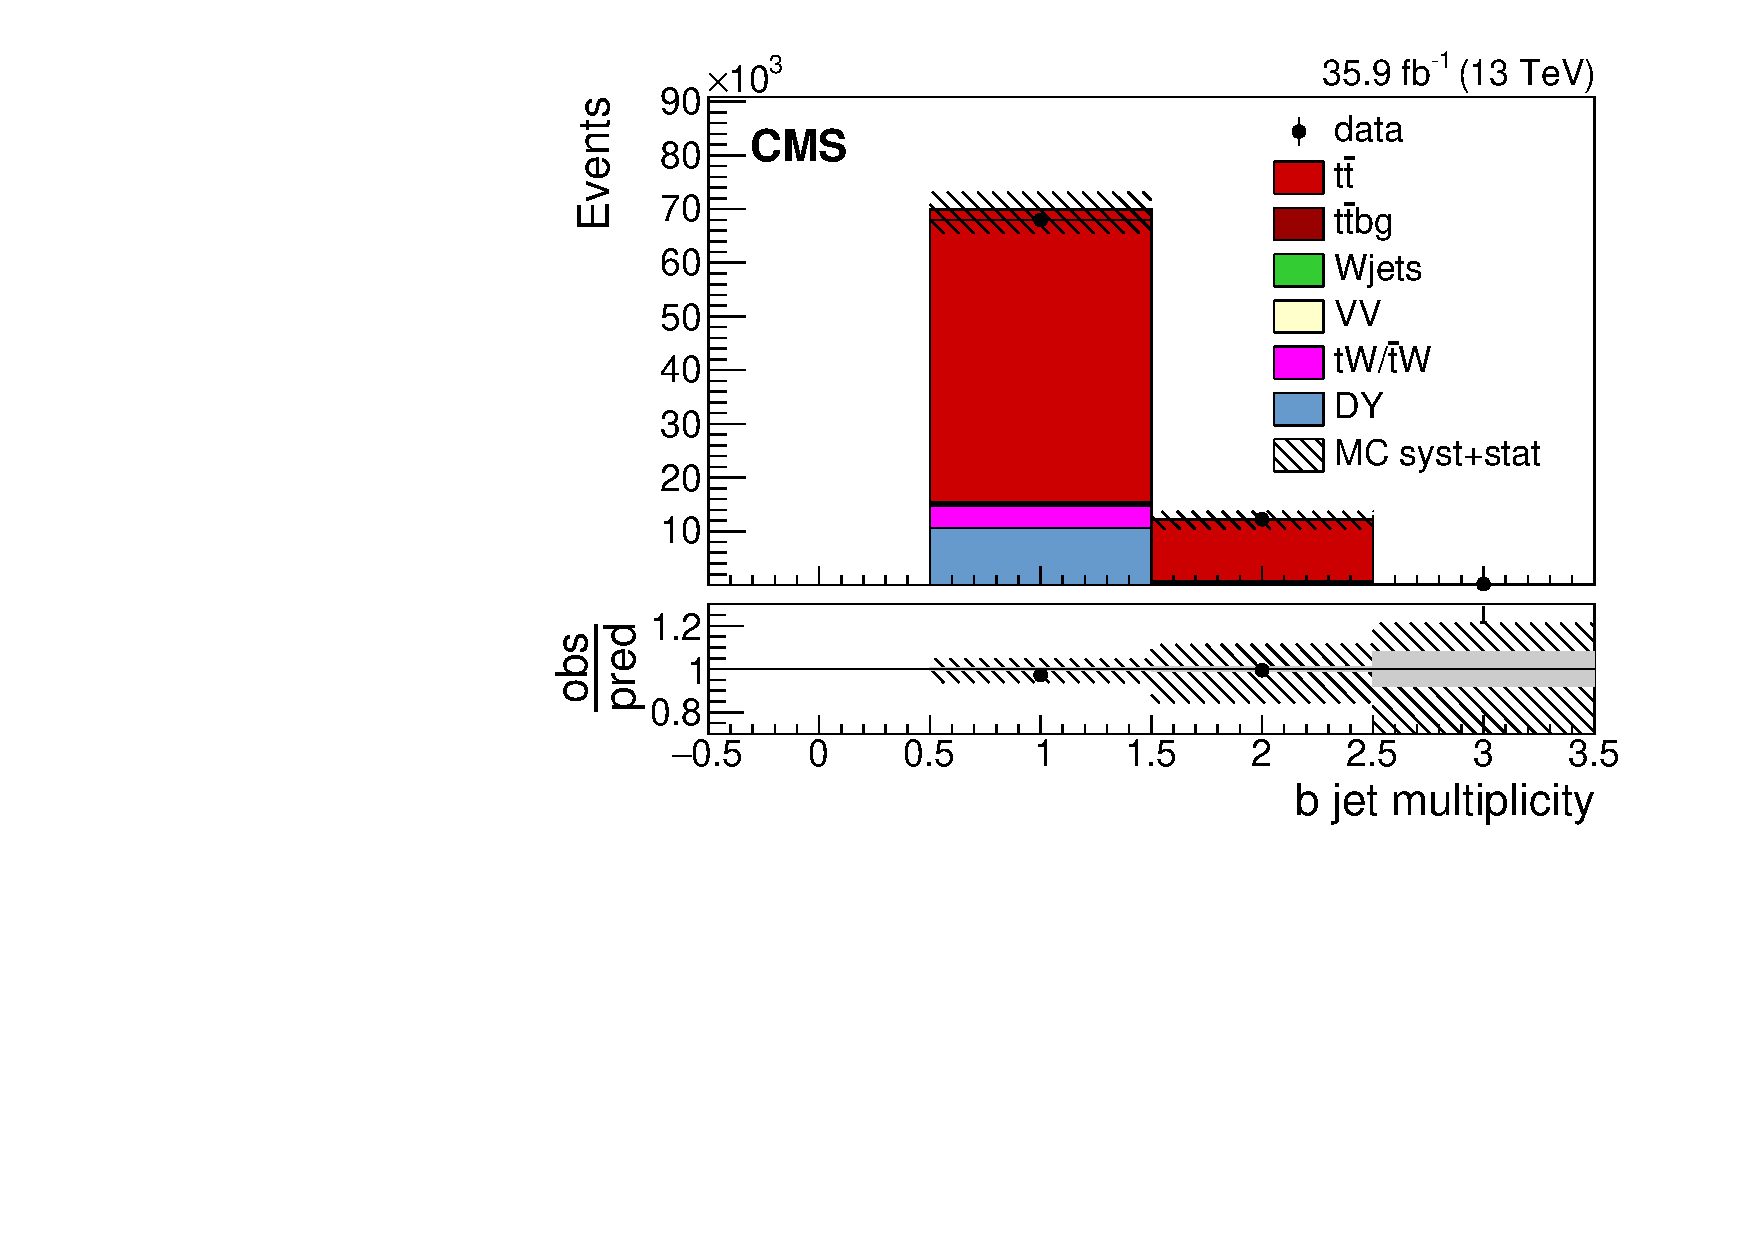
\includegraphics{CrossSection/Figures/ControlPlots/mumu_sysnom/selected_b-jet_multi_step_8.pdf}}
    \resizebox{0.48 \textwidth}{!}{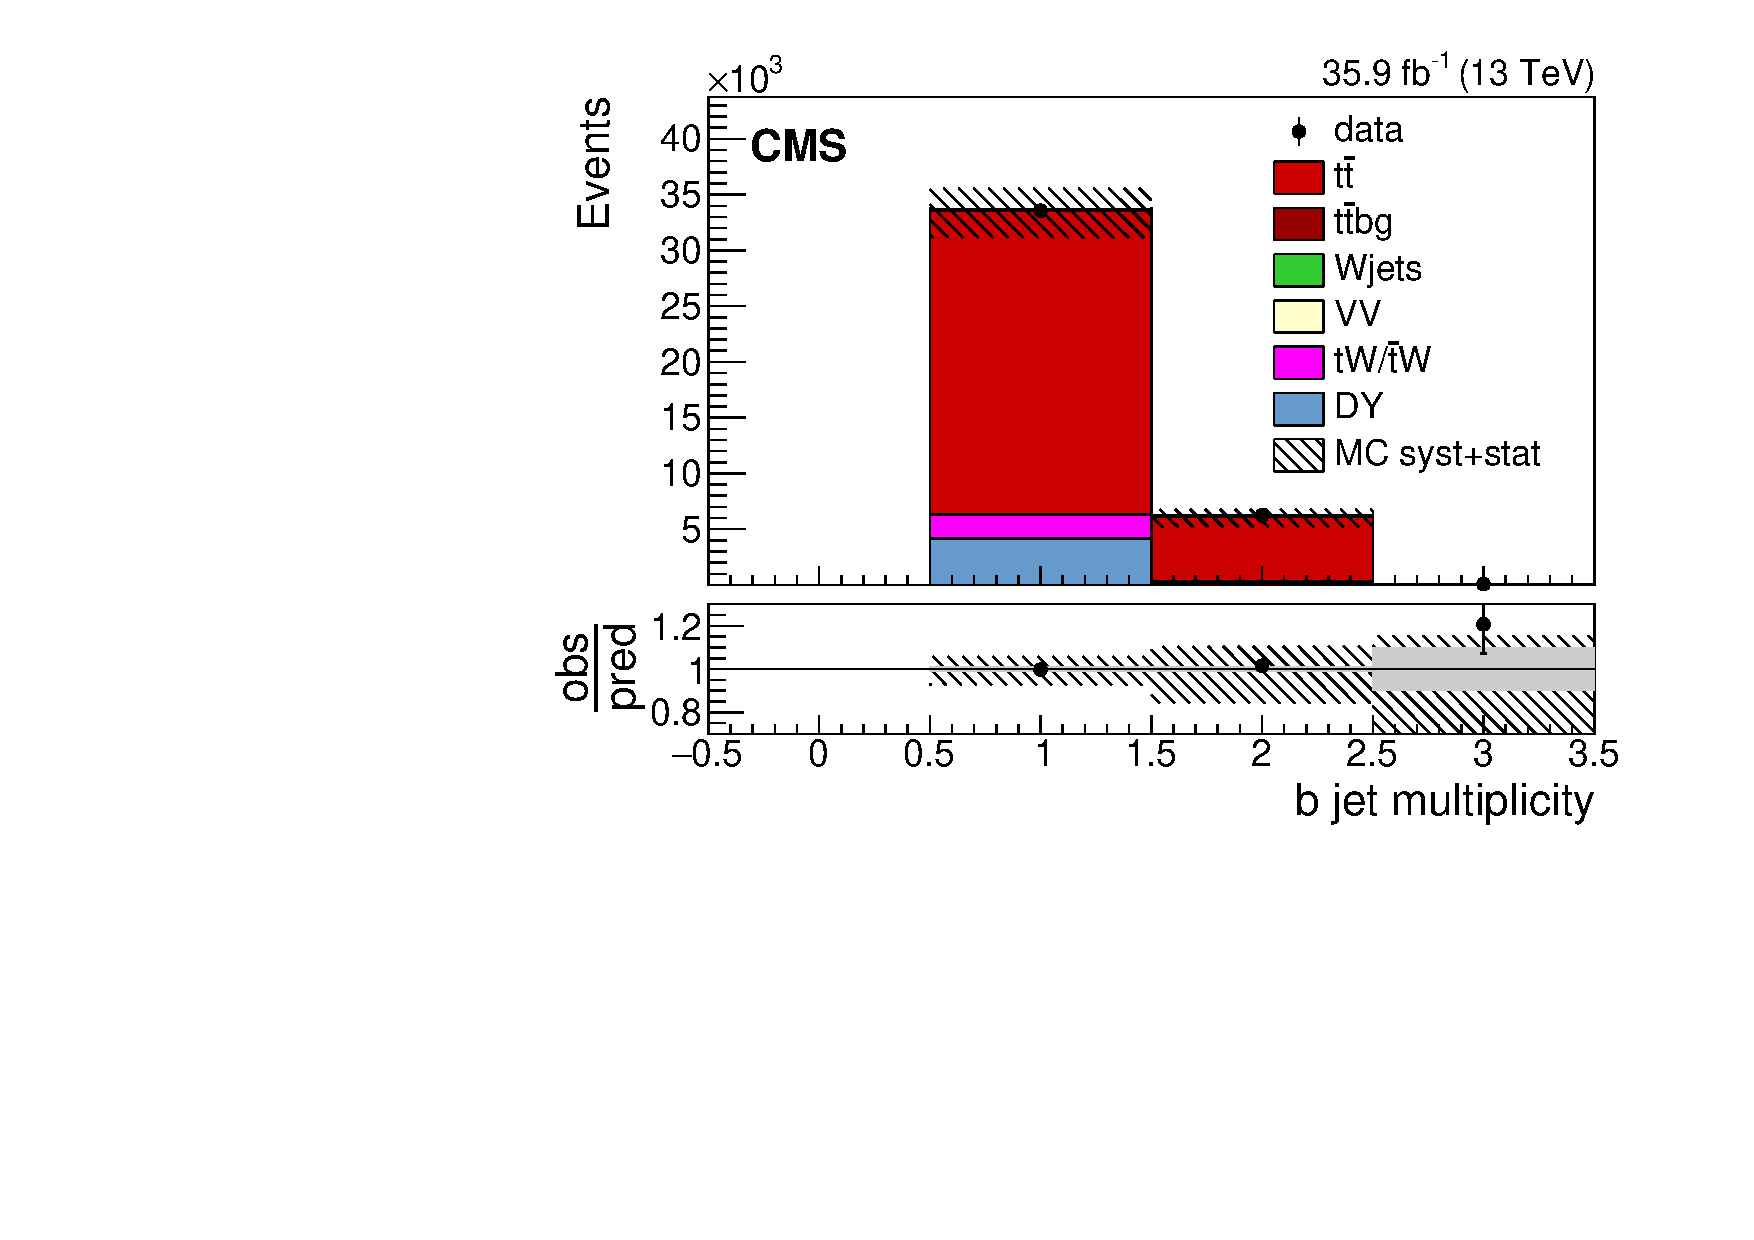
\includegraphics{CrossSection/Figures/ControlPlots/ee_sysnom/selected_b-jet_multi_step_8.pdf}}
    \caption{Number of b tagged jets \emu (upper left), \mumu (upper right) and \ee (lower row) decay channels.
        The events are shown after the
        event selection.  The hatched
        bands correspond to the total uncertainty on the sum of the
        predicted yields. 
        %agrohsje , excluding luminosity and background
        %normalization uncertainties. 
        The ratios of data to the sum of the predicted yields are
        shown at the bottom pannel of each plot. The solid gray band
        represents the contribution of the statistical uncertainty.}  
       \label{fig:xsec_bjets_ctrplots}
  \end{center}
\end{figure}


The invariant mass of the dilepton system is shown in Figure \ref{fig:xsec_ctrplots_mll} for the \emu channel and depending on the number of b-tagged jets (for zero, one and two or more b tagged jets).
The distribution for signal events has a broad peak in the region of $60-100 \; \GeV$ with long tails up to $300 \; \GeV$.
Drell-Yan events show the expected peak at the mass of the Z boson.
The distributions again show the reduction of the  Drell-Yan contribution when more b-tagged jets are required.

Together the comparisons of event yield distributions between measurment and prediction for several variables show agrement between measurement and prediction.
A few remaining regions of phase space where they do not agree are well understood and the discrepancy is covered by systematic uncertainties.
The agreements shows that the simulation is sufficiently reliable to be used for the further measurement.


\begin{figure}[htbp!]
  \begin{center}
    \resizebox{0.48 \textwidth}{!}{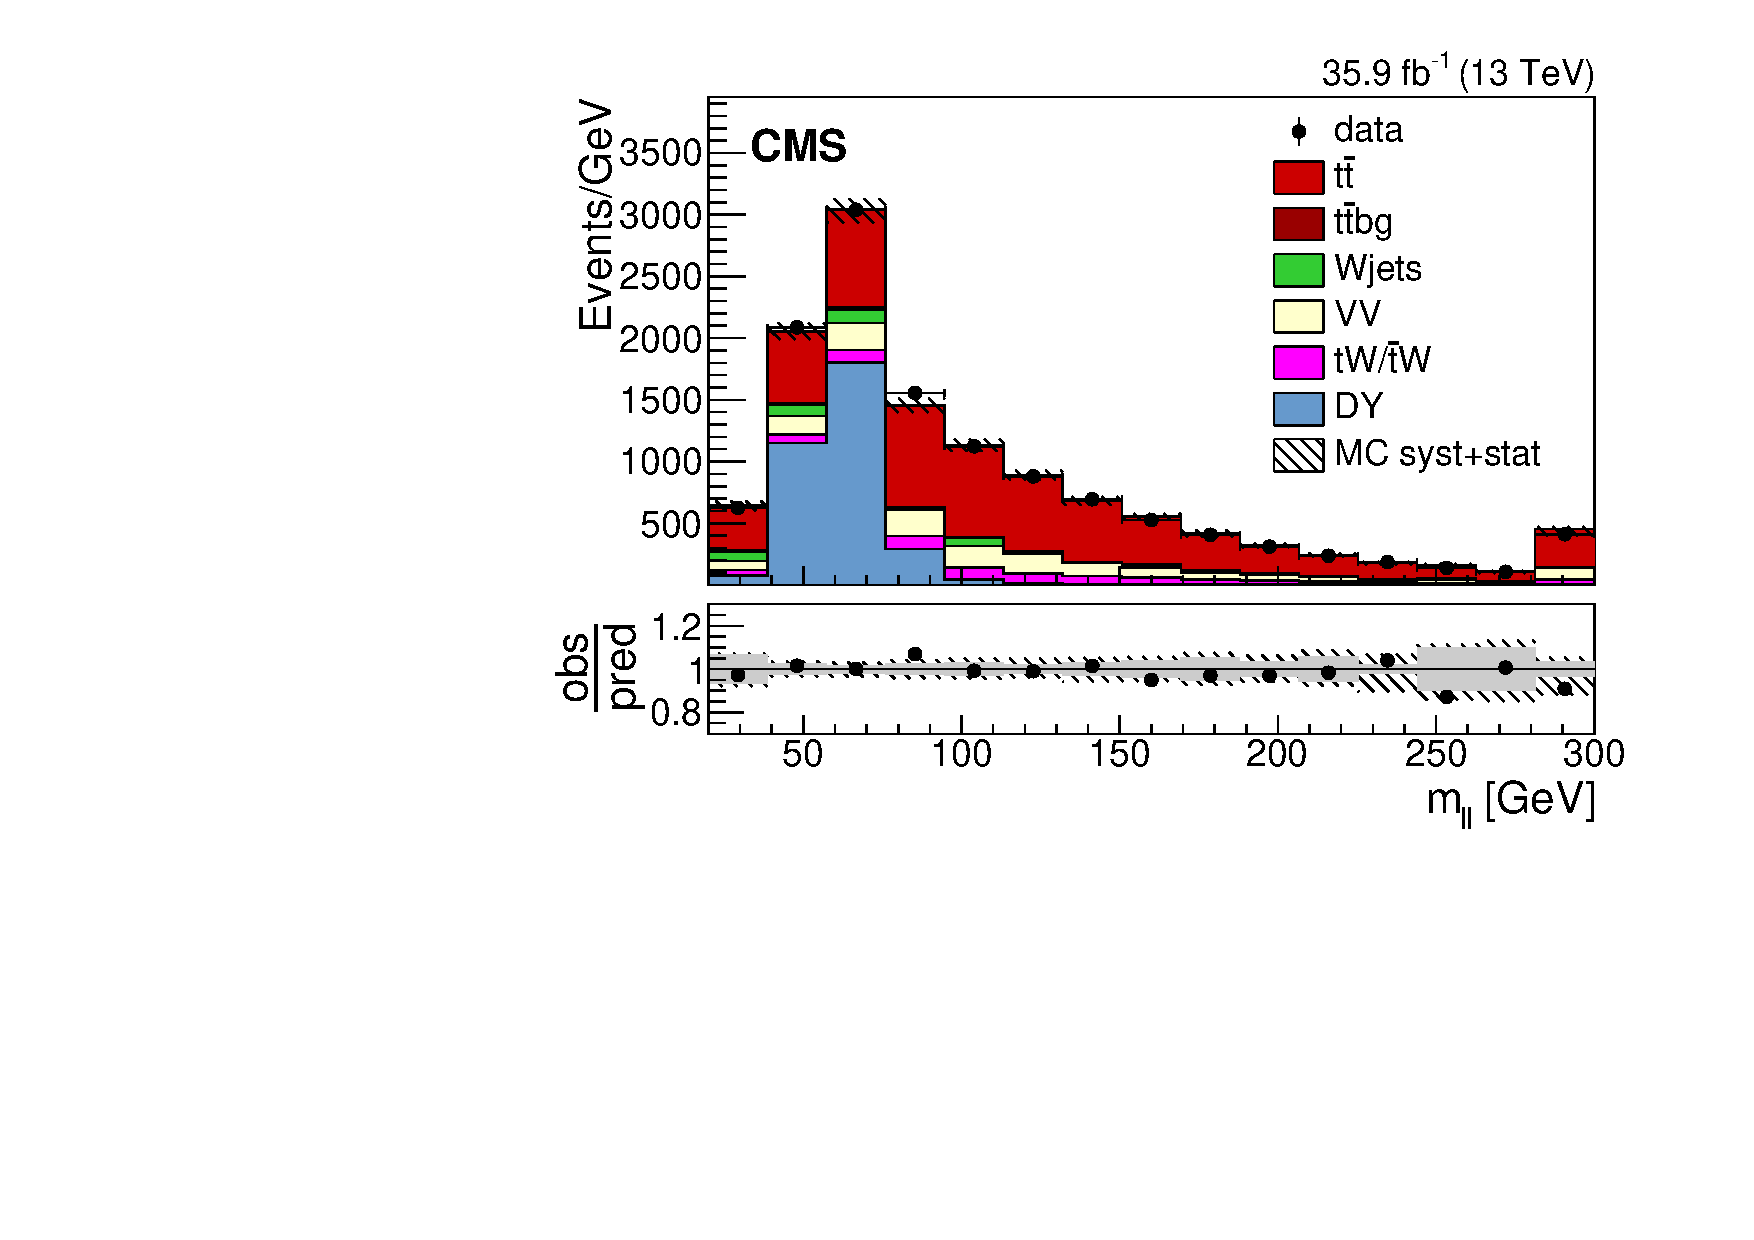
\includegraphics{CrossSection/Figures/ControlPlots/emu_sysnom/mll_0_b-jets_step_8.pdf}}
    \resizebox{0.48 \textwidth}{!}{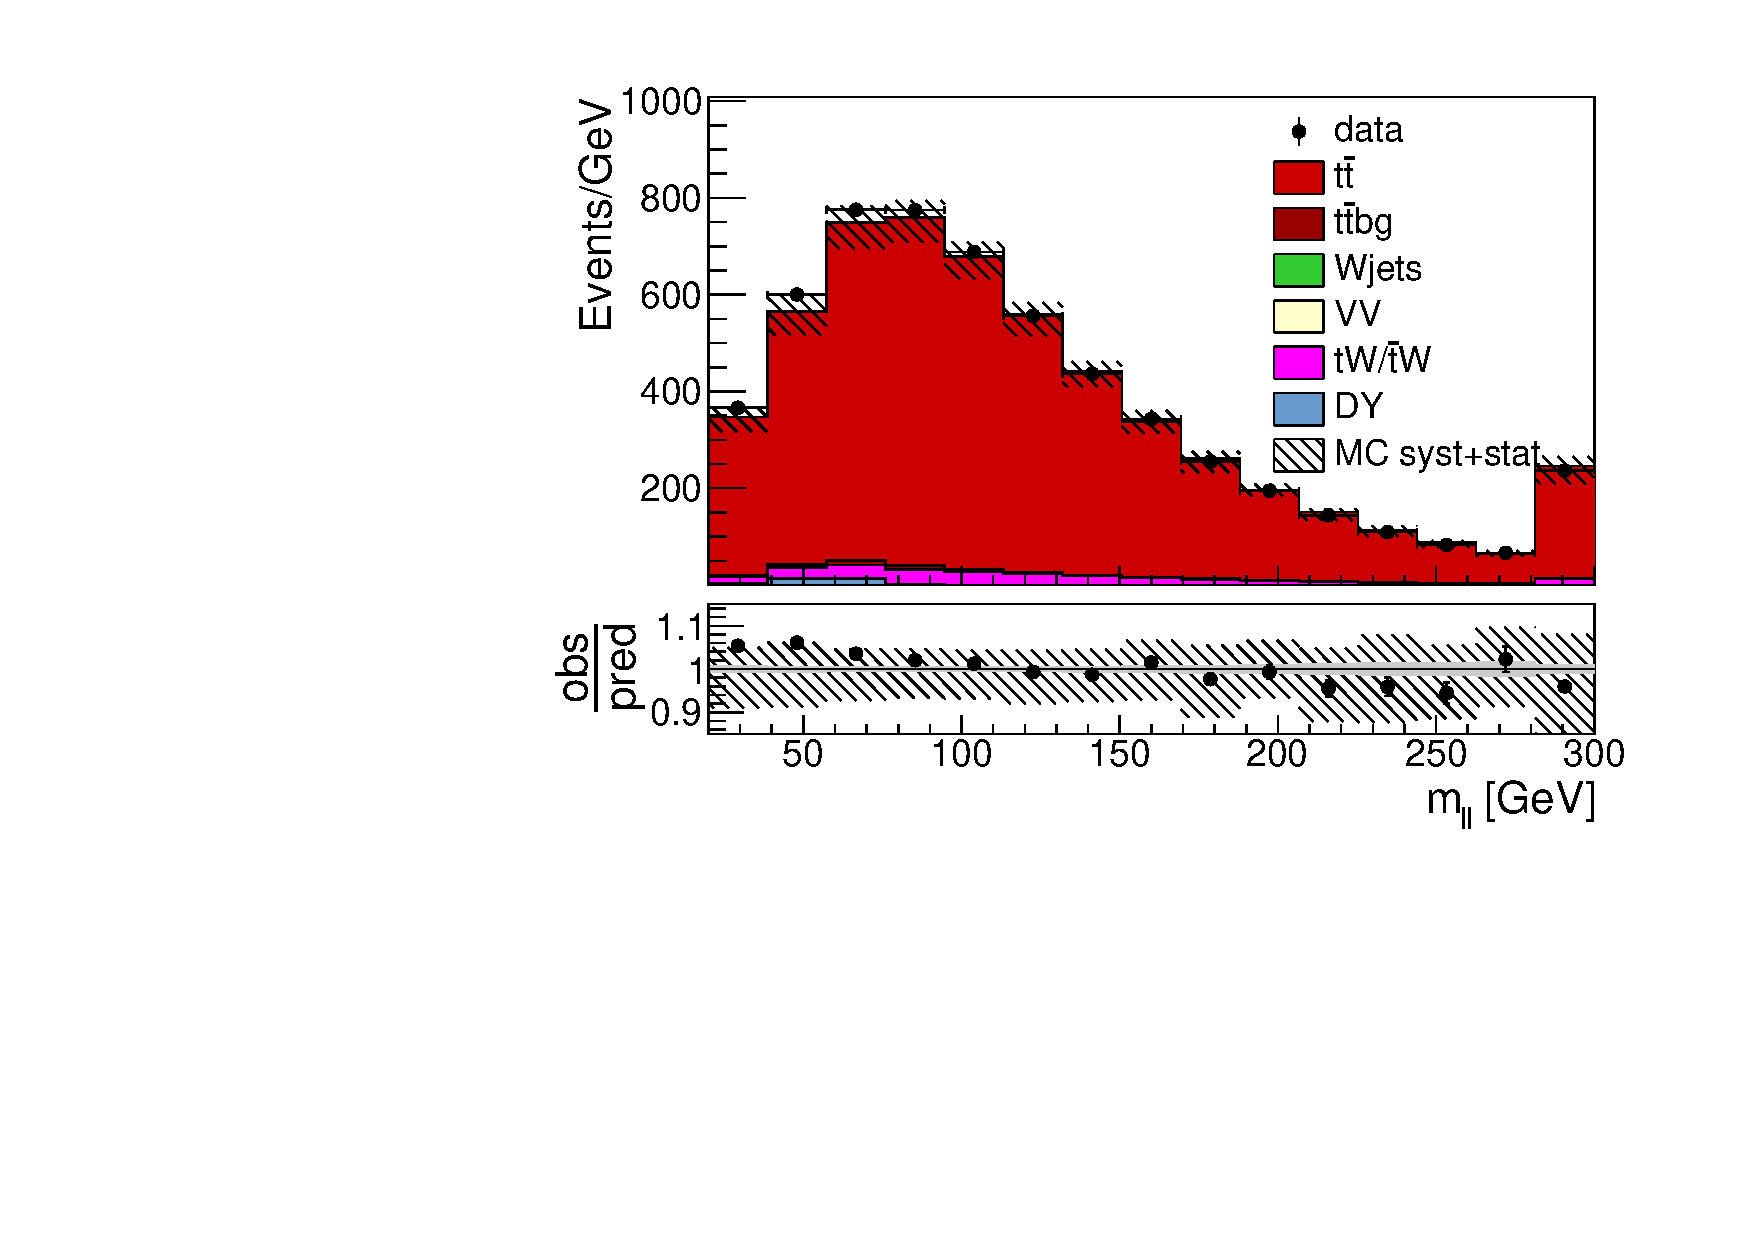
\includegraphics{CrossSection/Figures/ControlPlots/emu_sysnom/mll_1_b-jets_step_8.pdf}}
    \resizebox{0.48 \textwidth}{!}{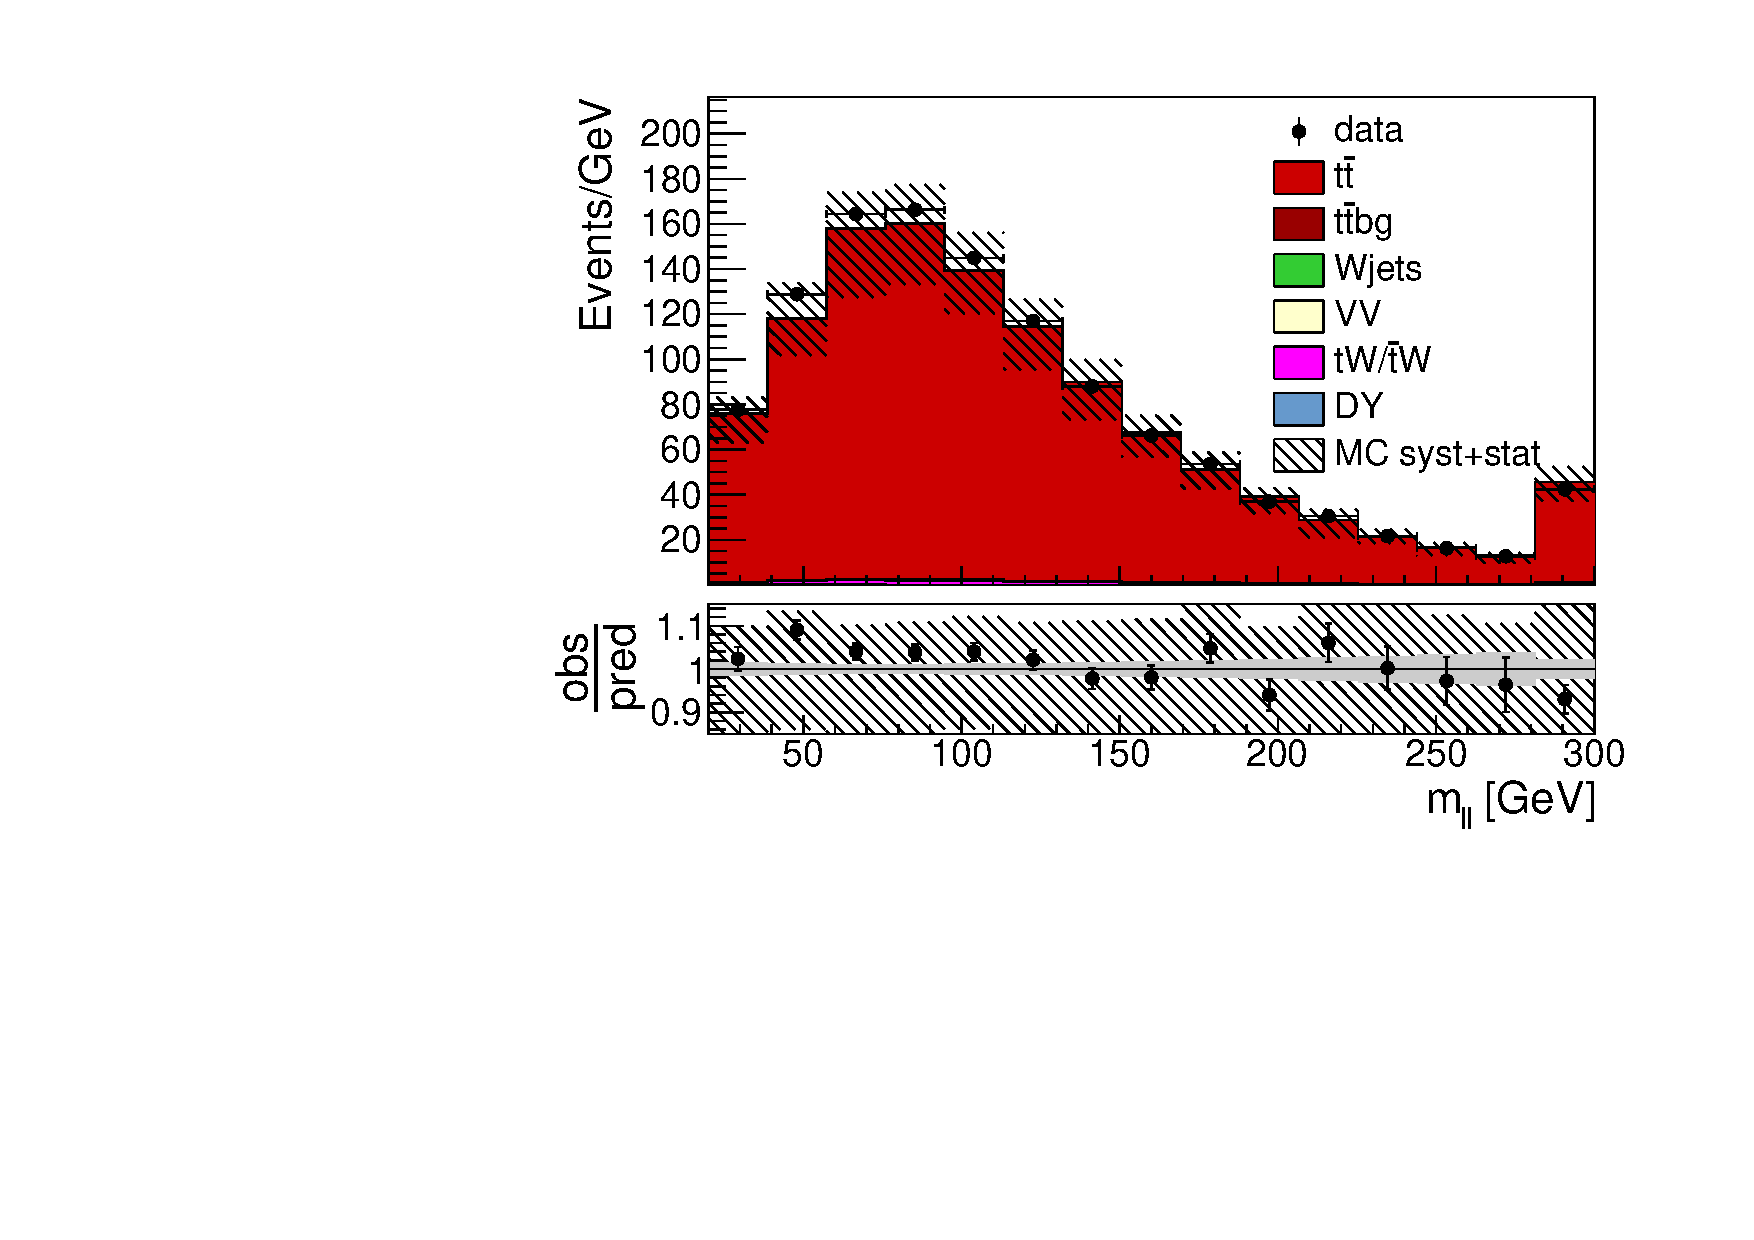
\includegraphics{CrossSection/Figures/ControlPlots/emu_sysnom/mll_2_b-jets_step_8.pdf}} \\
      \caption{Invariant mass of the dilepton system with zero (upper left), one (upper right) and two (lower row) b-tagged 
      jets in the \emu channel. The hatched
        bands correspond to the total uncertainty on the sum of the
        predicted yields. 
        %agrohsje , excluding luminosity and background
        %normalization uncertainties. 
        The ratios of data to the sum of the predicted yields are
        shown at the bottom pannel of each plot. The solid gray band
        represents the contribution of the statistical uncertainty.}  
       \label{fig:xsec_ctrplots_mll}
  \end{center}
\end{figure}



\section{Choice of Event Categories and Template Distributions}
\label{sec:xsec_templates}


In order to increase the separation between signal and background the events are divided according to the number of b-tagged jets.
There are three categories of events with one, two and zero or more than two b-tagged jets.
This further categorisation also allows to determine the efficiency to find a b-tagged jet in a signal event using the topology of \ttbar decays.
Since each of the top quarks decays into a W boson and a b quark it can be assumed that every \ttbar event should contain two jets originating from a b quark.
Decays of a top quark to a W boson and a light quark can be considered negligible.
Therefore, the amount of \ttbar events with less than two b tagged jets can be used to measure the efficiency to select a b tagged jet.

In this way the b-tagging efficiency can be determined independently for data and simulation. The efficiency of the b-tagging algorithm is independent of the rest of the event, so it can be assumed to be the same in all \ttbar decay channels.
This in-situ measurement of the b-tagging efficiency in the phase space of the measurement is also expected to reduce the impact of the uncertainties on the b-tagging efficiency on the final measurement of the \ttbar cross section.

Beside the number of b-jets, the number of light (non b-tagged) jets is one of the main discriminators between \ttbar and background events.
Events containing a top quark pair tend to have a higher amount of additional jets from final state radiation. The main background for all three channels is Drell-Yan where the Z boson in the final state can not radiate additional gluons, 
which cause additional jets.
Events are split according to the number of light jets for one, two and zero or more than 2 jets.
In each event the the \pt of the trailing light jet is chosen as template distribution.
Together with the \pt of the light jets their multiplicity is sensitive to the systematic uncertainty on the response of the jet reconstruction and
the systematic uncertainties introduced by theoretical assumptions in the simulation.

The separation of events into the \emu,\mumu and \ee channels is explained with the selection in Section \ref{sec:xsec_sel}. The \ttbar production cross section does not depend on the decay, so the cross section is assumed to be constant in all three decay channels.
By simultaneously fitting the three channels the two uncorrelated lepton identification efficiencies $\epsilon_e$ and $\epsilon_\mu$ are correlated with each other. 
These correlations can be illustrated by the relation between the number of \ttbar events in each dilepton channel ($s_{\emu}$, $s_{ee}$ and $s_{\mu\mu}$), the ttbar cross section (\stt) and the lepton 
efficiencies, which is shown in simplified form in Equation \ref{eq:xsec_lepsplit}.
\begin{eqnarray}
s_{e \mu}  &\propto& \stt \epsilon_{e} \epsilon_{\mu}  \\
s_{ee}  &\propto&  \stt \epsilon_{e}^2  \\
s_{\mu \mu}  &\propto&  \stt \epsilon_{\mu}^2
\label{eq:xsec_lepsplit}.
\end{eqnarray}
These relations can be written as: 

\begin{equation}
\frac{s_{\mu\mu}}{s_{ee}} \propto \frac{\epsilon_{\mu}^2}{\epsilon_{e}^2} \vspace{0.4cm} \frac{s_{\mu\mu}}{s_{e\mu}} \propto \frac{\epsilon_{\mu}}{\epsilon_{e}}
\label{eq:xsec_lepeffs}
\end{equation}

The number of events in each channels is known within uncertainties, so the lepton efficiencies are correlated are with each other.
When determnining the \ttbar cross section the ratio of the lepton efficiencies is implicitly constrained in the fit.
Since the uncertainties on the lepton efficiencies are uncorrelated the constraints of the efficiency ratio constrains the higher of the two lepton efficiency uncertainties.
Here, prior to the fit, the muon identification uncertainty is smaller, and thus in the fit the single-electron identification uncertainty is constrained to that of the muon.

In summary, events are divided by the dilepton decay channel into the \emu, \ee and \mumu categories. Then they are separated according to the number of b-tagged jets into events with one, two and zero or more b-tagged jets. 
For the same-flavour channels (\ee, \mumu) only events with more than one b-tagged jet are considered to supress the large amount of Drell-Yan background events. The resulting seven categories are further subdivided according to the number of additional jets (not b-tagged) into events with zero,one,two or three or more additional jets.
The final 28 templates are listed in Table \ref{tab:xsec_templates} and shown in Figures 
 \ref{fig:xsec_emu_inputdistr}, \ref{fig:xsec_mumu_inputdistr} and \ref{fig:xsec_ee_inputdistr} for the \emu, \mumu and \ee channel respectively.

\begin{table}[htbp!]
\begin{center}
\caption{Table of the template distributions chosen for the fit. They are listed for each of the three decay channels and are further split according to the number
of b tagged jets and additional non b-tagged jets.~\label{tab:xsec_templates}}
\begin{tabular}{c|l|l|l|l}
Number of b jets                      & Number of add. jets&   \multicolumn{3}{c}{Decay channel}                  \\
                                      &                    & \emu channel      & \mumu channel   & \ee channel \\
\hline
\multirow{3}{*}{0 or $\geq 3$ b jets} & 0 add. jets        & event yield       & -               & -            \\
                                      & 1 add. jets        & \pt (1st jet)     & -               & -            \\
                                      & 2 add. jets        & \pt (2nd jet)     & -               & -            \\
                                      & $\geq 3$ add. jets & \pt (trail. jet)  & -               & -            \\ 
\hline    
\multirow{3}{*}{1 b jet}              & 0 add. jets        & event yield       & event yield     & event yield  \\
                                      & 1 add. jets        & \pt (1st jet)     & event yield     & event yield  \\
                                      & 2 add. jets        & \pt (2nd jet)     & event yield     & event yield   \\
                                      & $\geq 3$ add. jets & \pt (trail. jet)  & event yield     & event yield   \\ 
\hline
\multirow{3}{*}{2 b jets}              & 0 add. jets        & event yield       & event yield     & event yield  \\
                                      & 1 add. jets        & \pt (1st jet)     & \pt (1st jet)   & \pt (1st jet) \\
                                      & 2 add. jets        & \pt (2nd jet)     & \pt (2nd jet)   & \pt (2nd jet) \\
                                      & $\geq 3$ add. jets & \pt (trail. jet)  & \pt (trail. jet)& \pt (trail. jet) \\                                 


\end{tabular}
\end{center}
\end{table}


\begin{figure}[htbp!]
  \begin{center}
    \resizebox{0.32 \textwidth}{!}{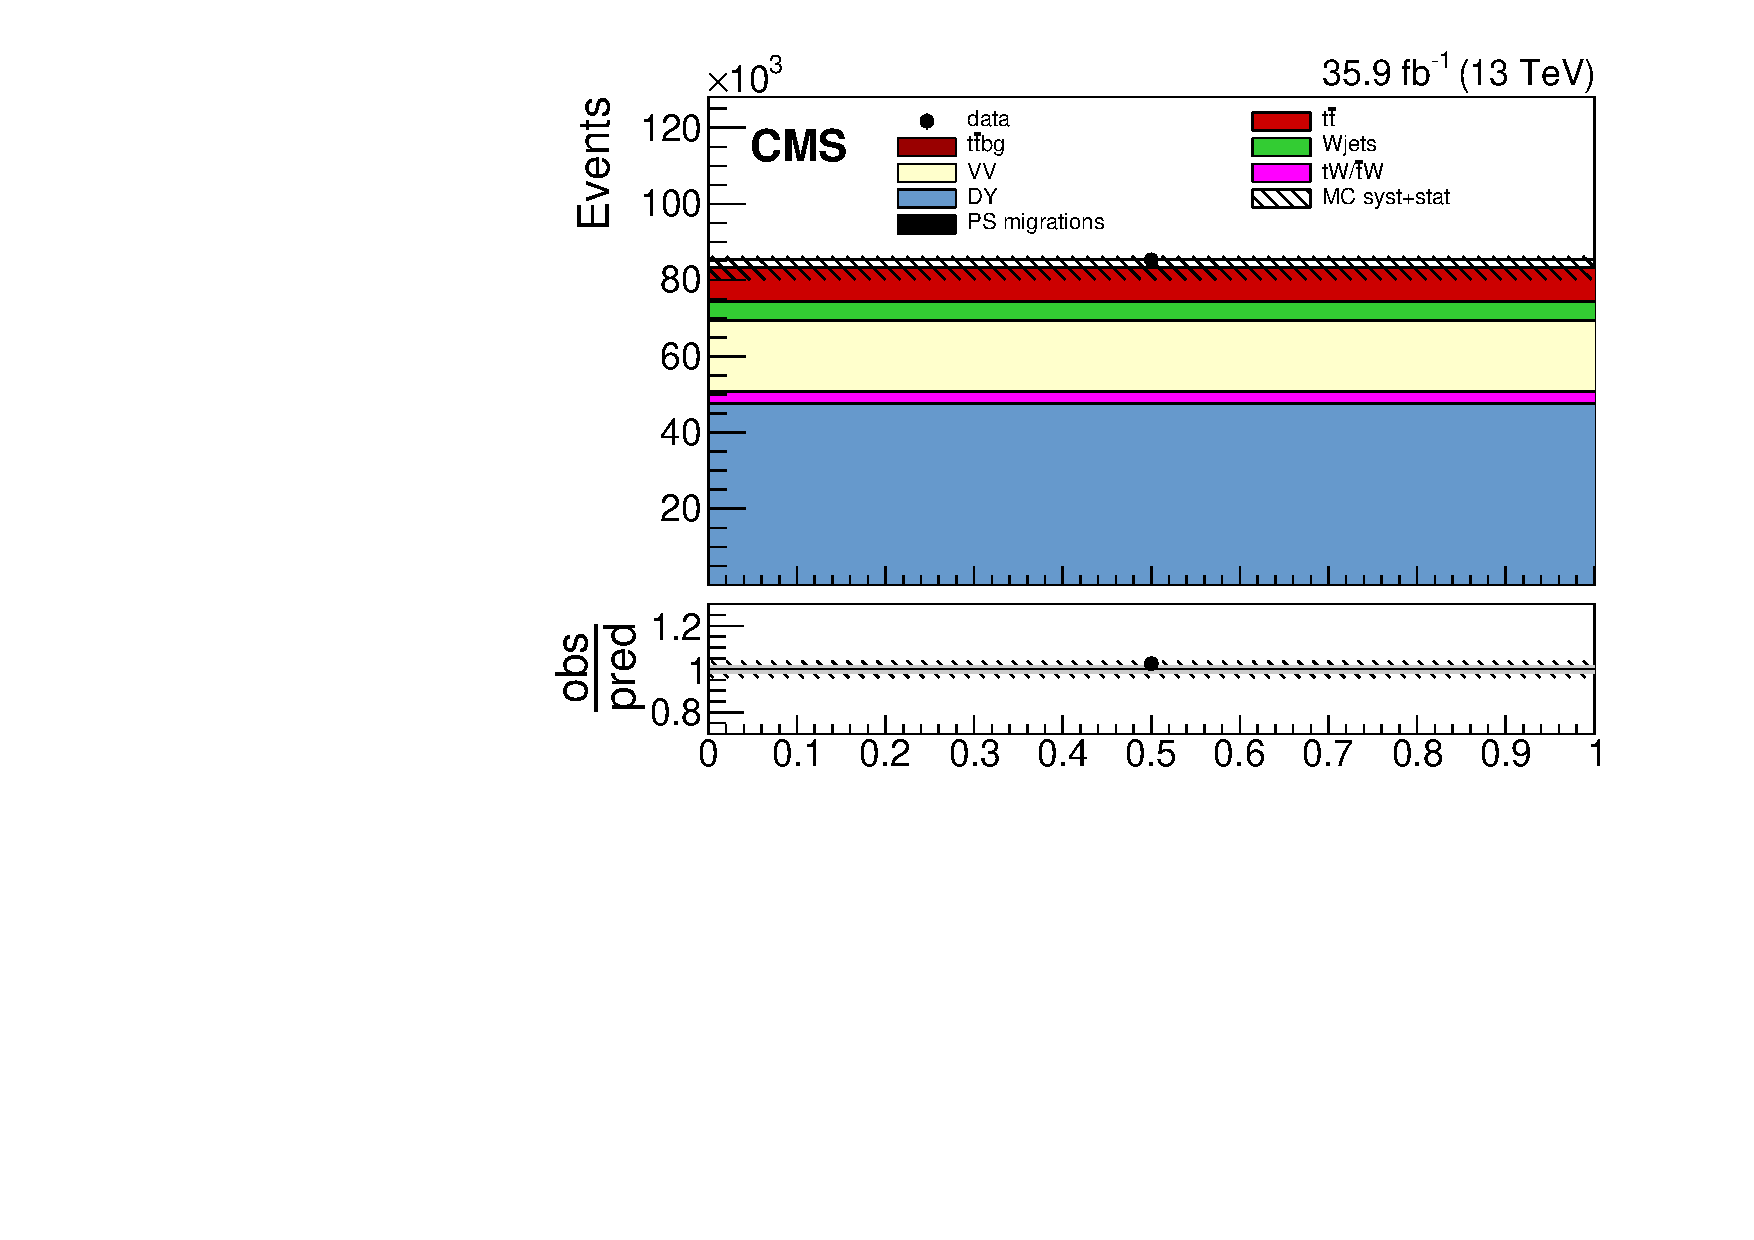
\includegraphics{CrossSection/Figures/ControlPlots/emu_sysnom/total_0_0_b-jets_step_8.pdf}}
    \resizebox{0.32 \textwidth}{!}{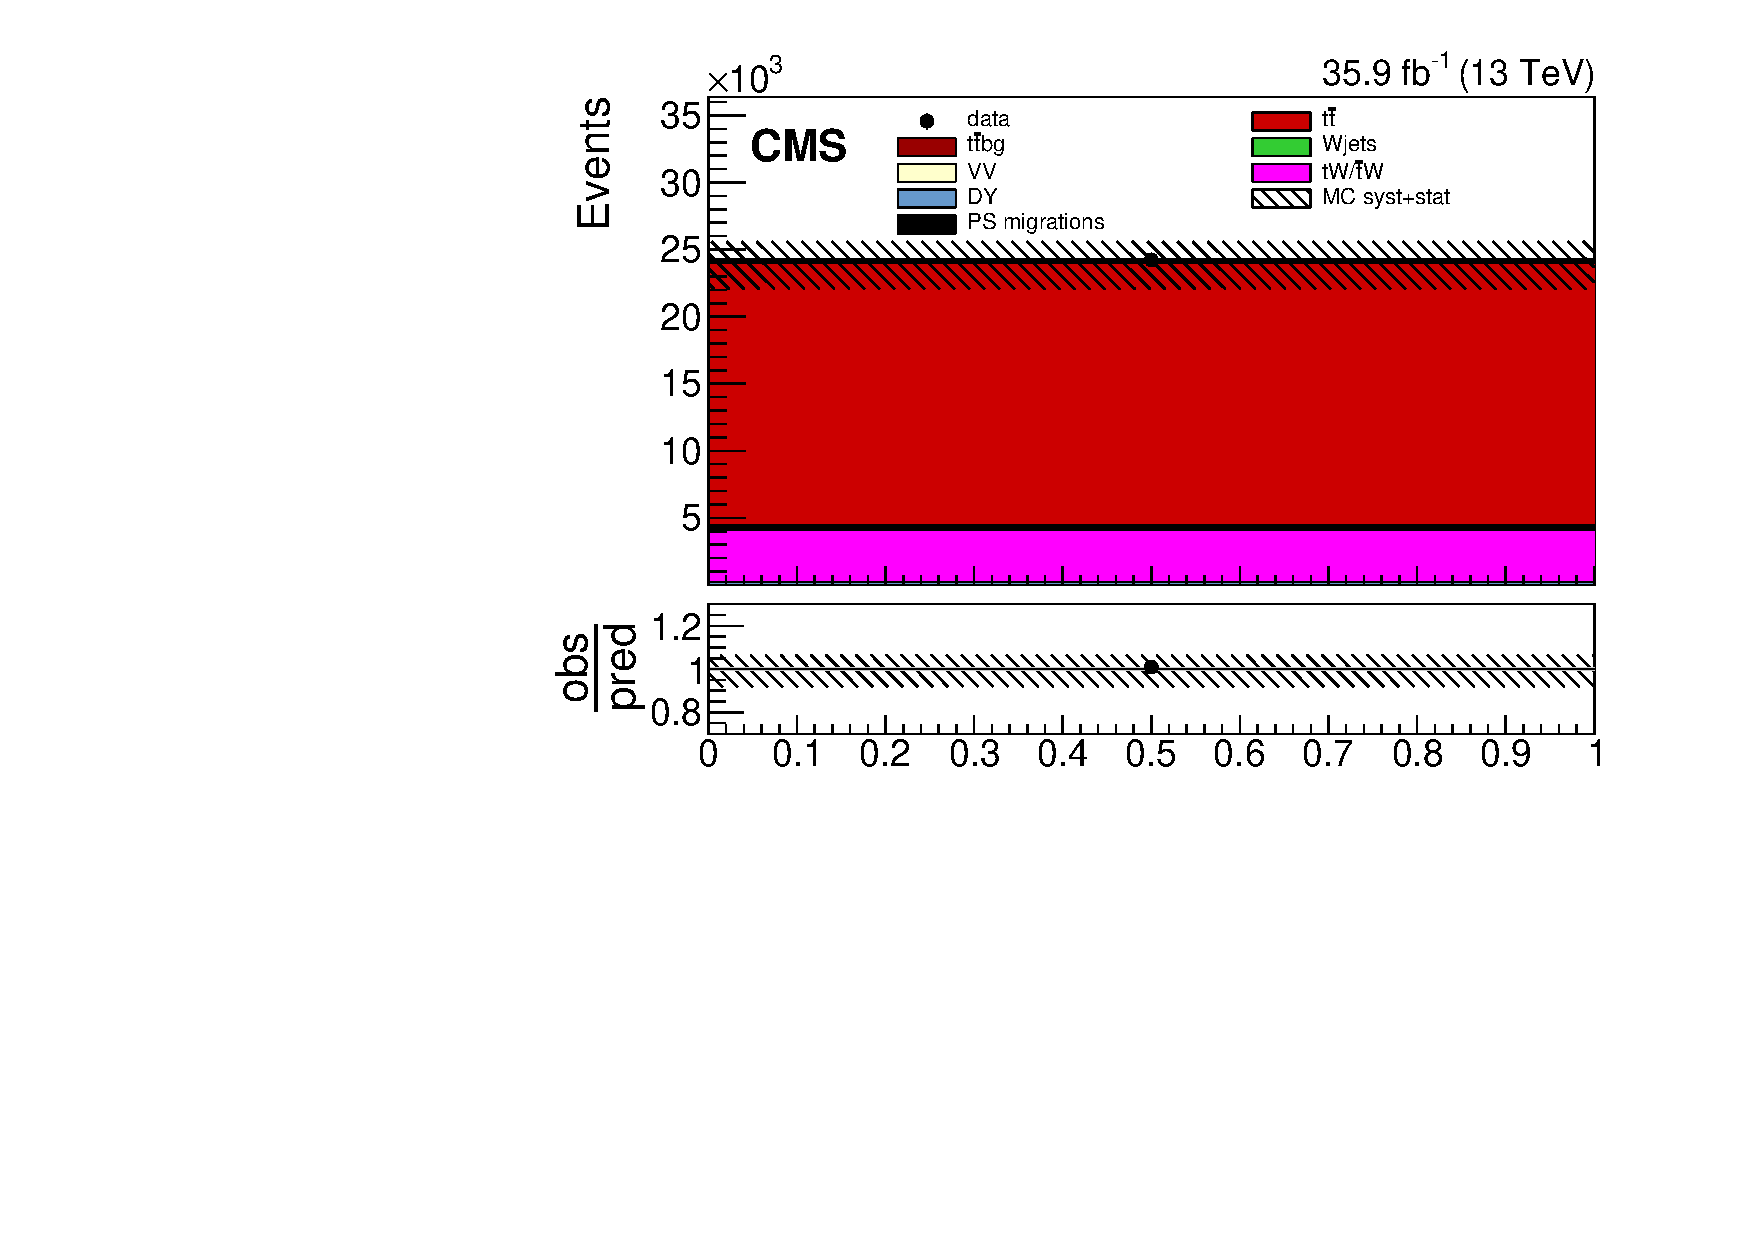
\includegraphics{CrossSection/Figures/ControlPlots/emu_sysnom/total_1_0_b-jets_step_8.pdf}}
    \resizebox{0.32 \textwidth}{!}{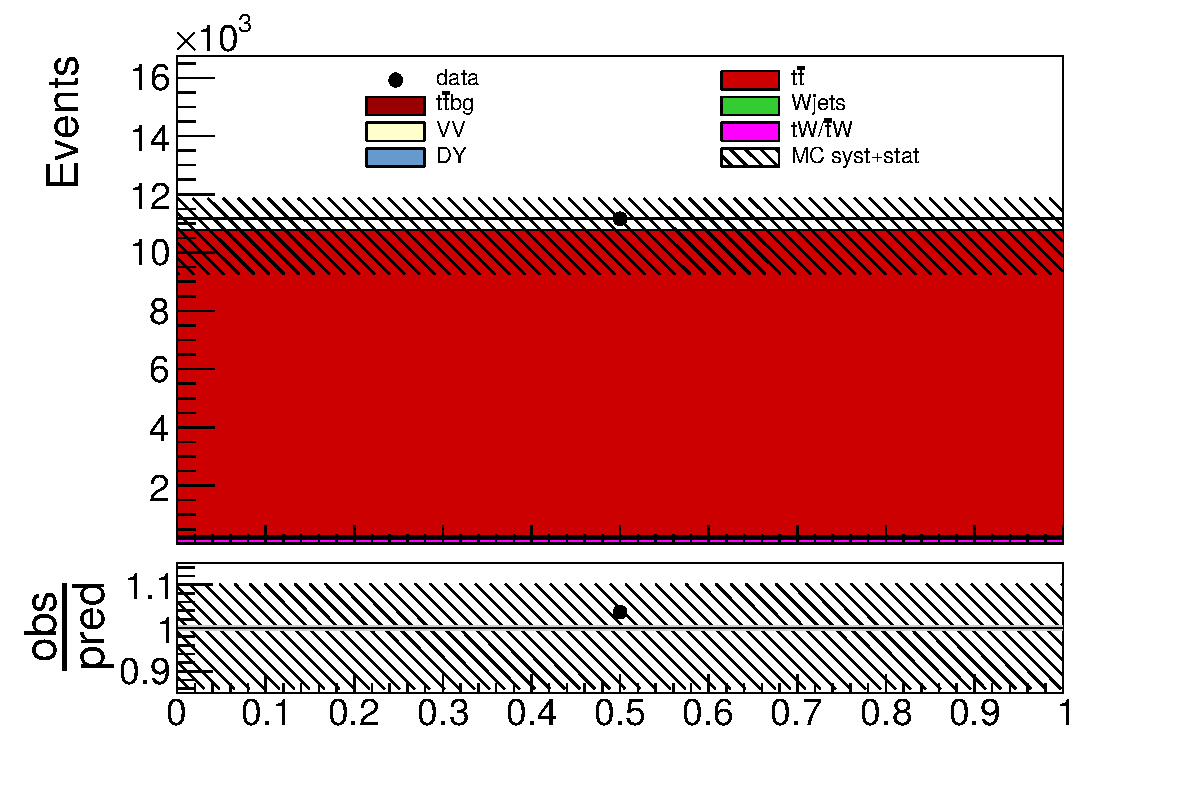
\includegraphics{CrossSection/Figures/ControlPlots/emu_sysnom/total_2_0_b-jets_step_8.pdf}}

    \resizebox{0.32 \textwidth}{!}{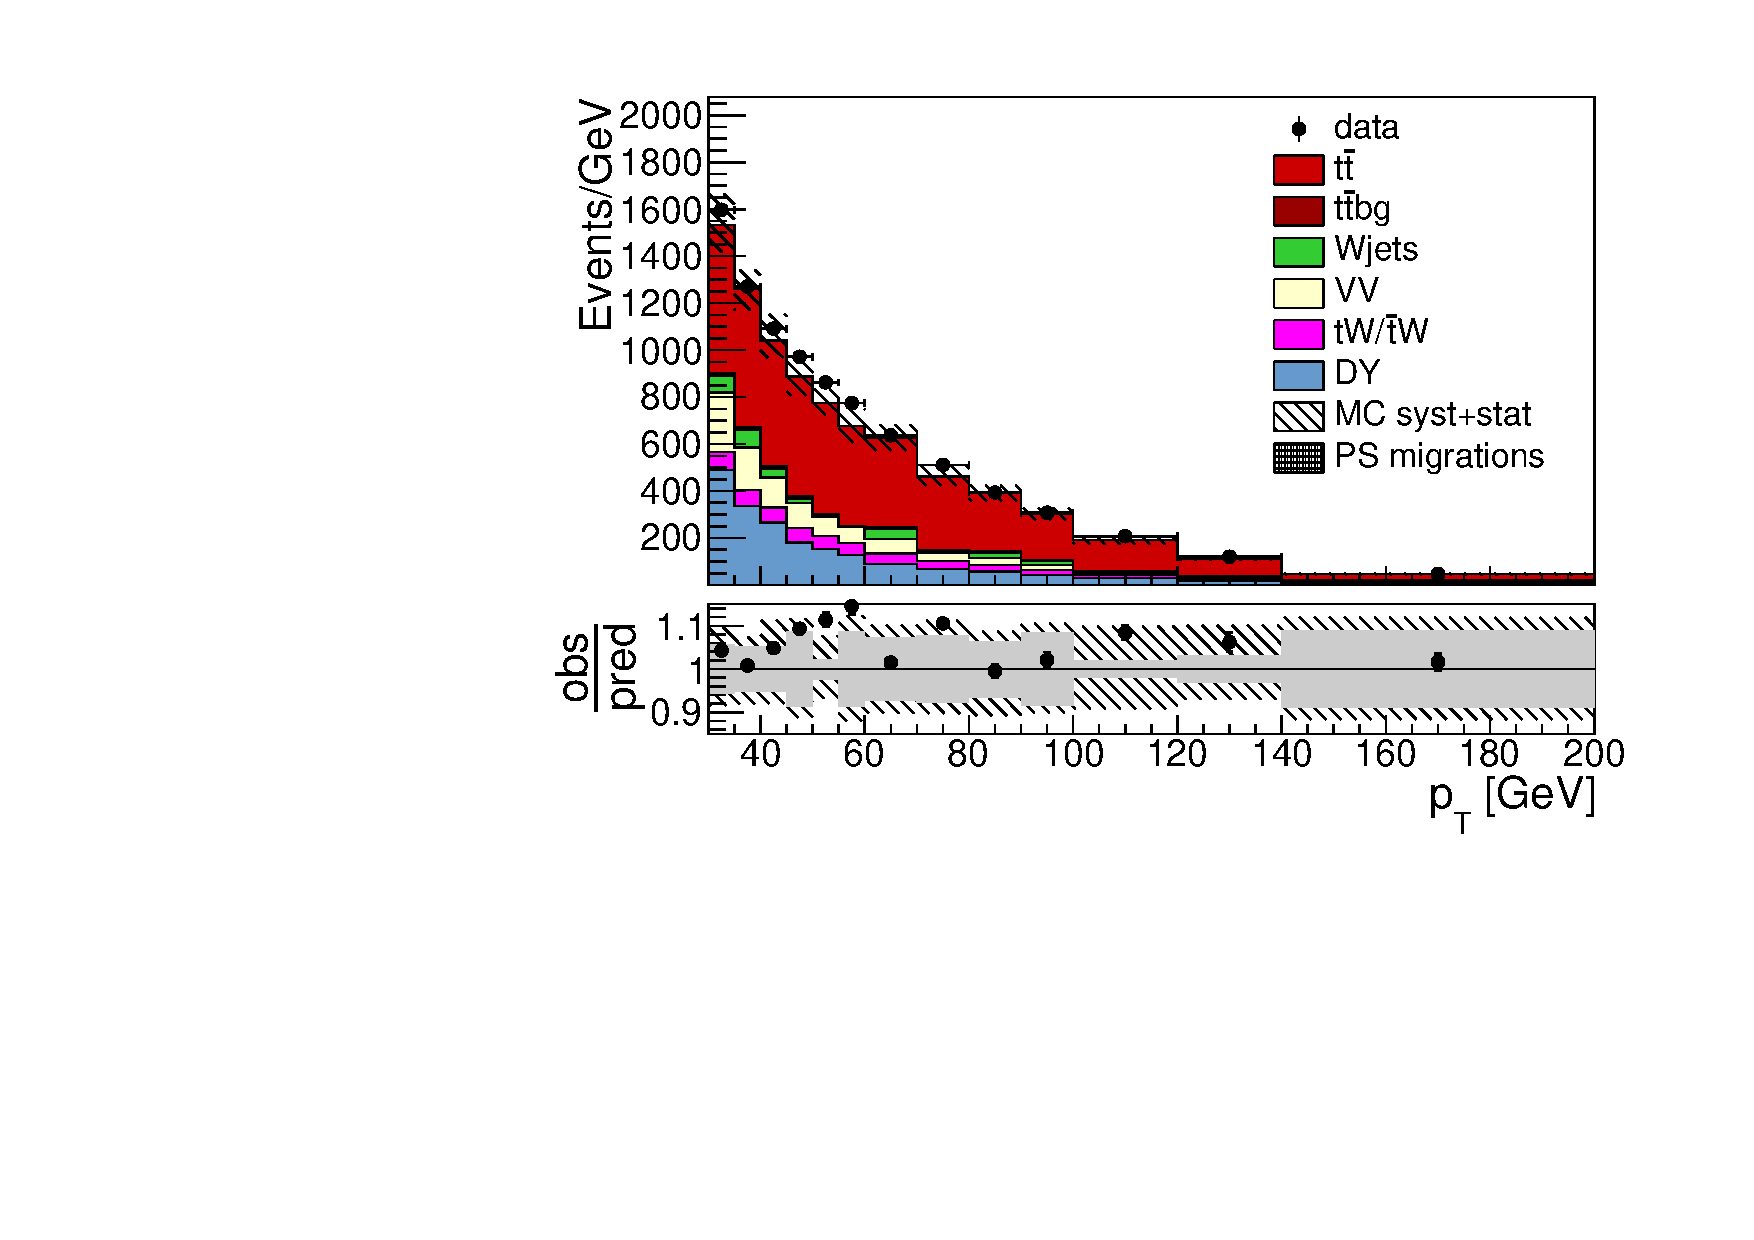
\includegraphics{CrossSection/Figures/ControlPlots/emu_sysnom/lead_jet_pt_0_1_b-jets_step_8.pdf}}
    \resizebox{0.32 \textwidth}{!}{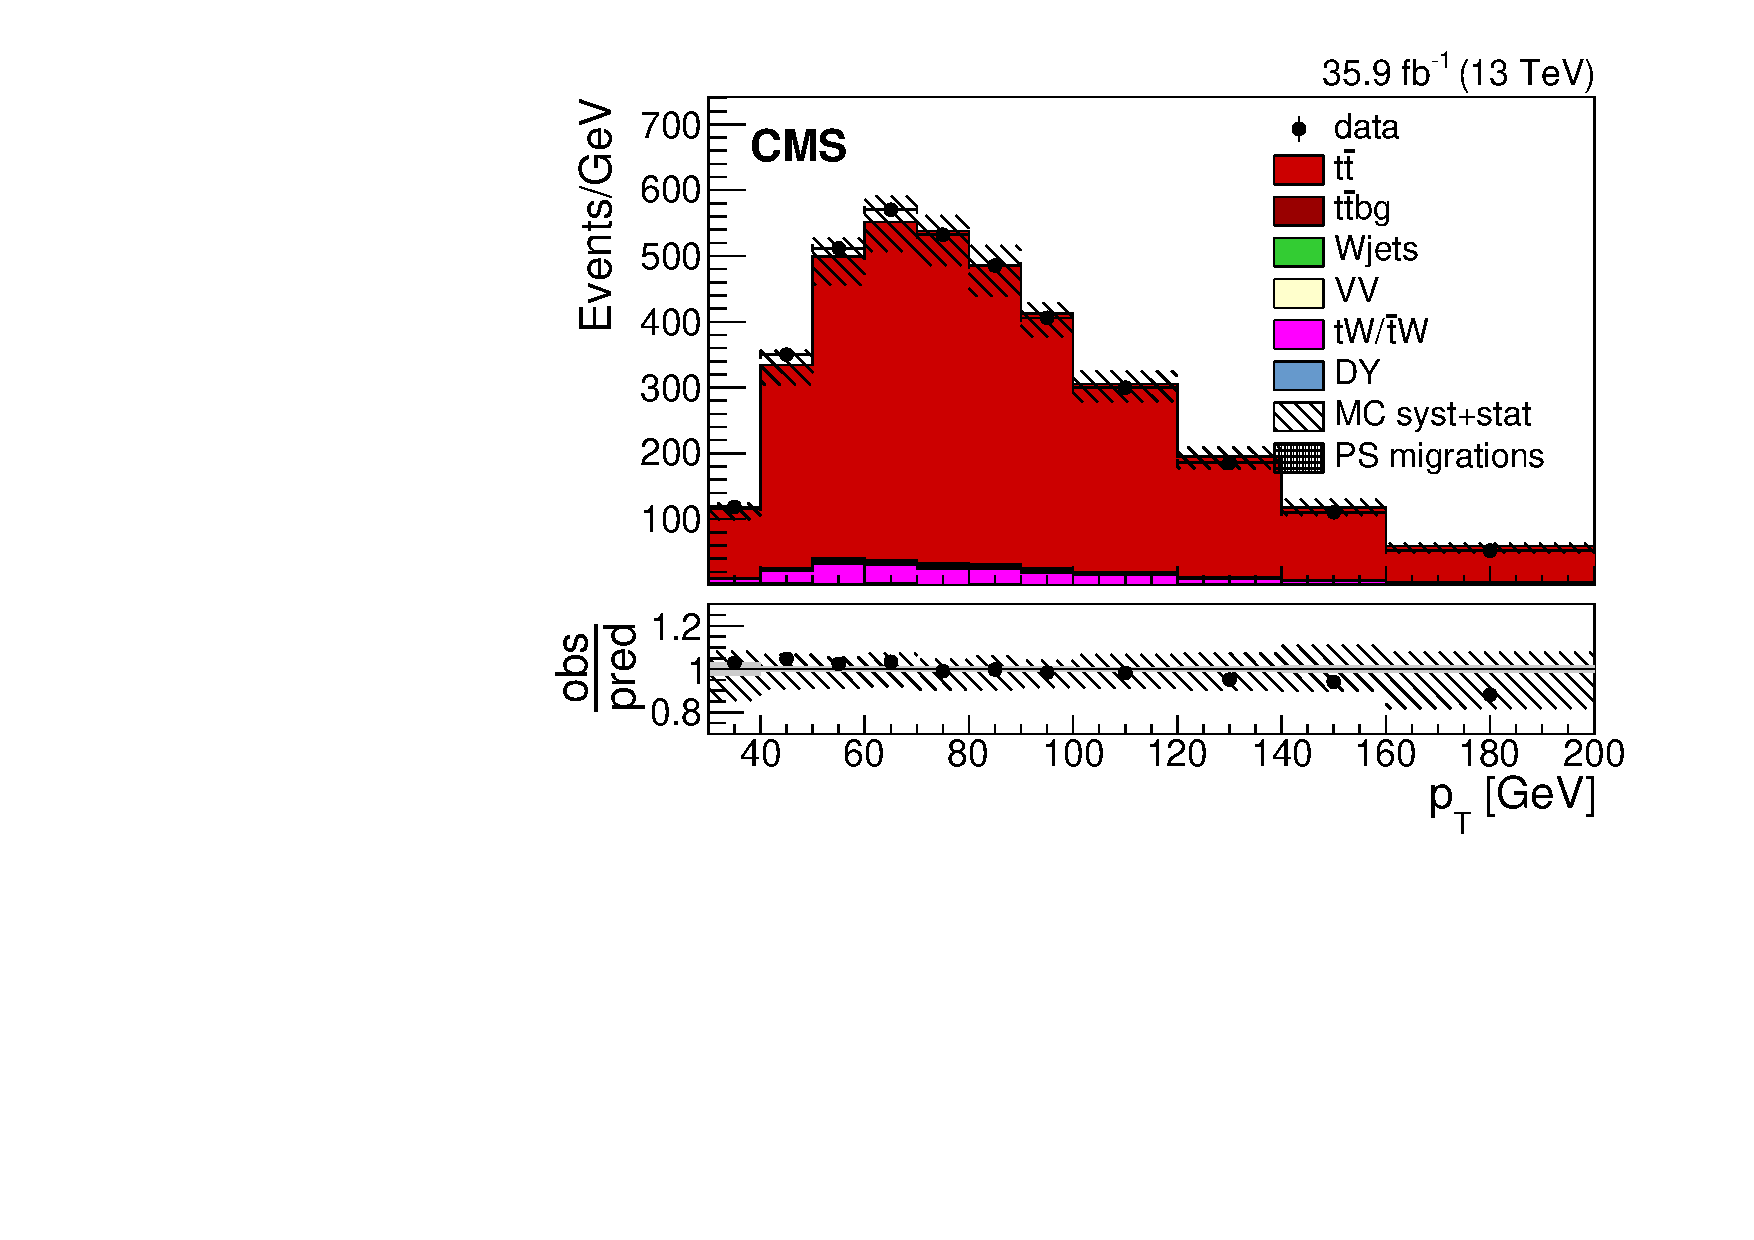
\includegraphics{CrossSection/Figures/ControlPlots/emu_sysnom/lead_jet_pt_1_1_b-jets_step_8.pdf}}
    \resizebox{0.32 \textwidth}{!}{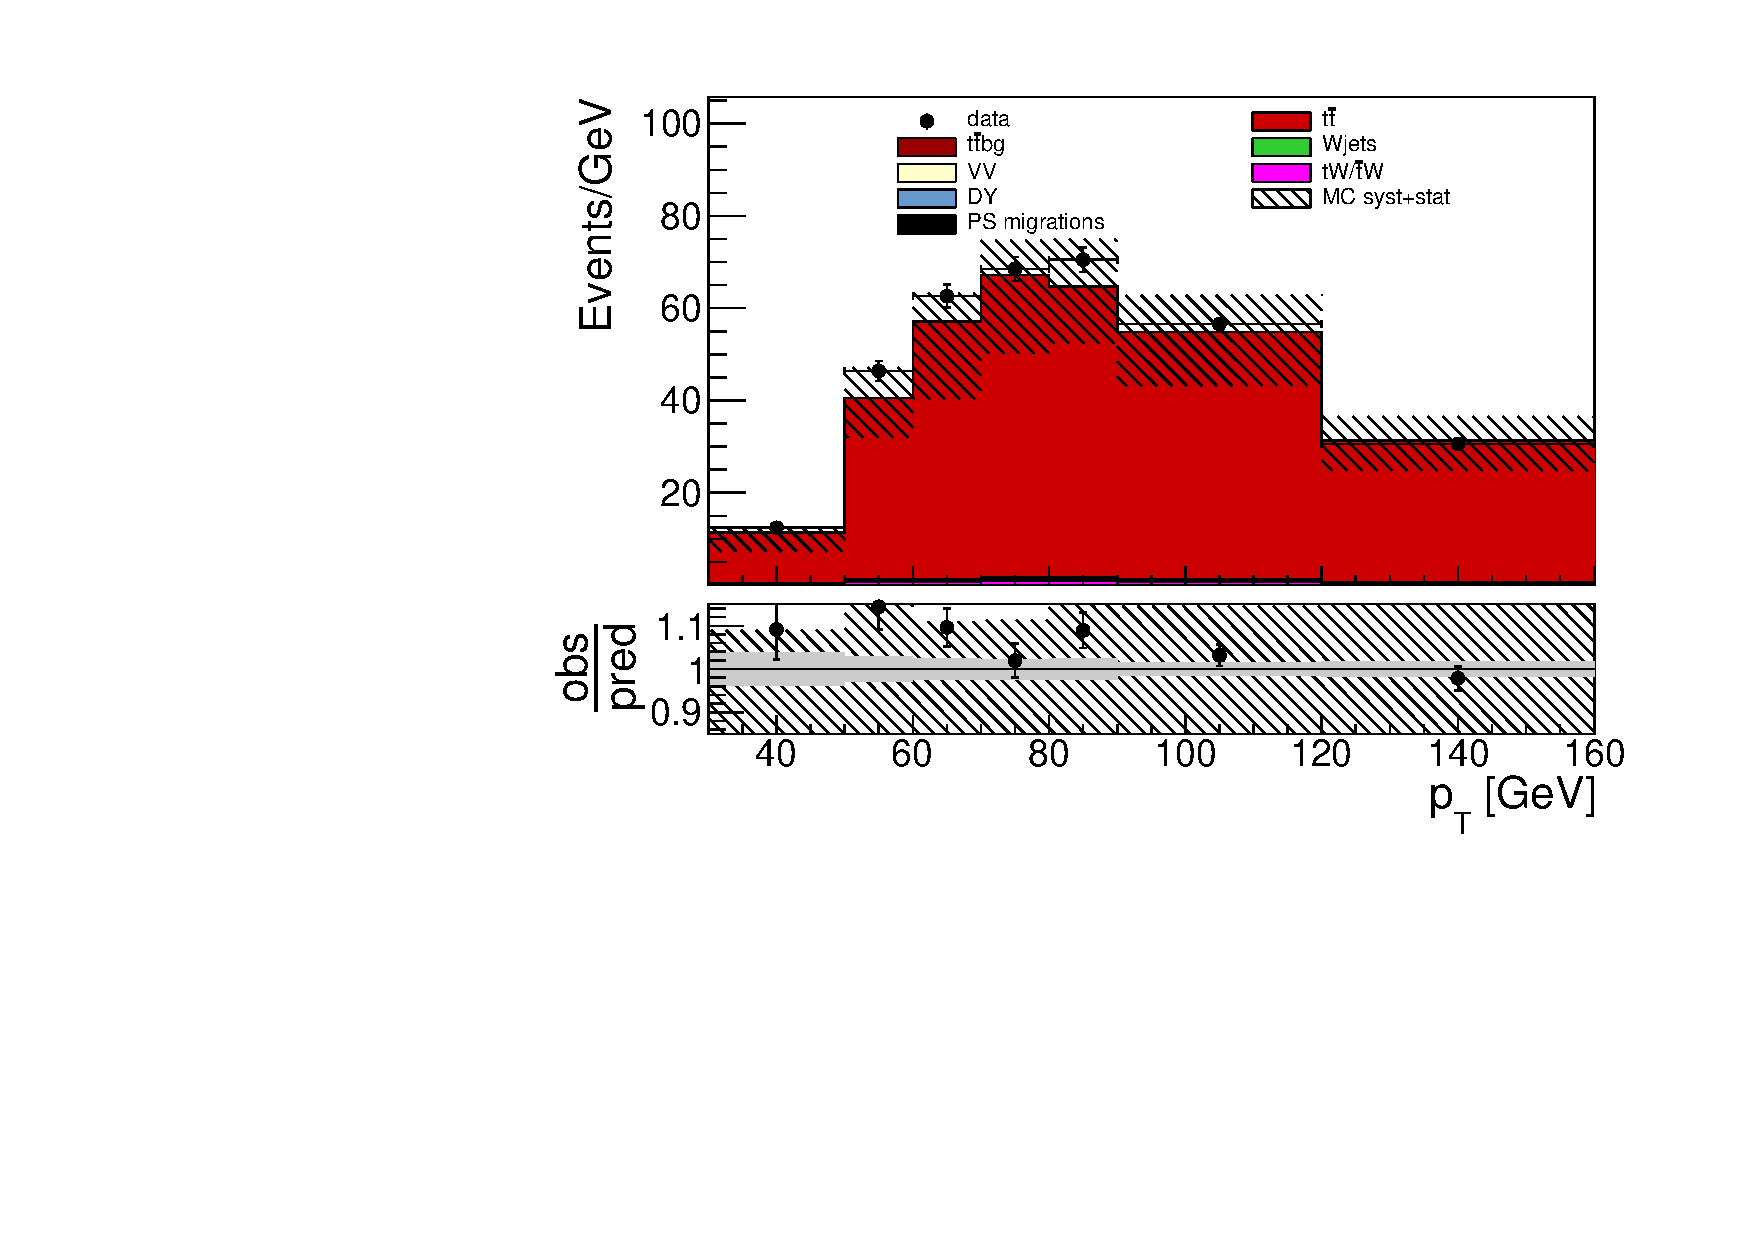
\includegraphics{CrossSection/Figures/ControlPlots/emu_sysnom/lead_jet_pt_2_1_b-jets_step_8.pdf}}
        
    \resizebox{0.32 \textwidth}{!}{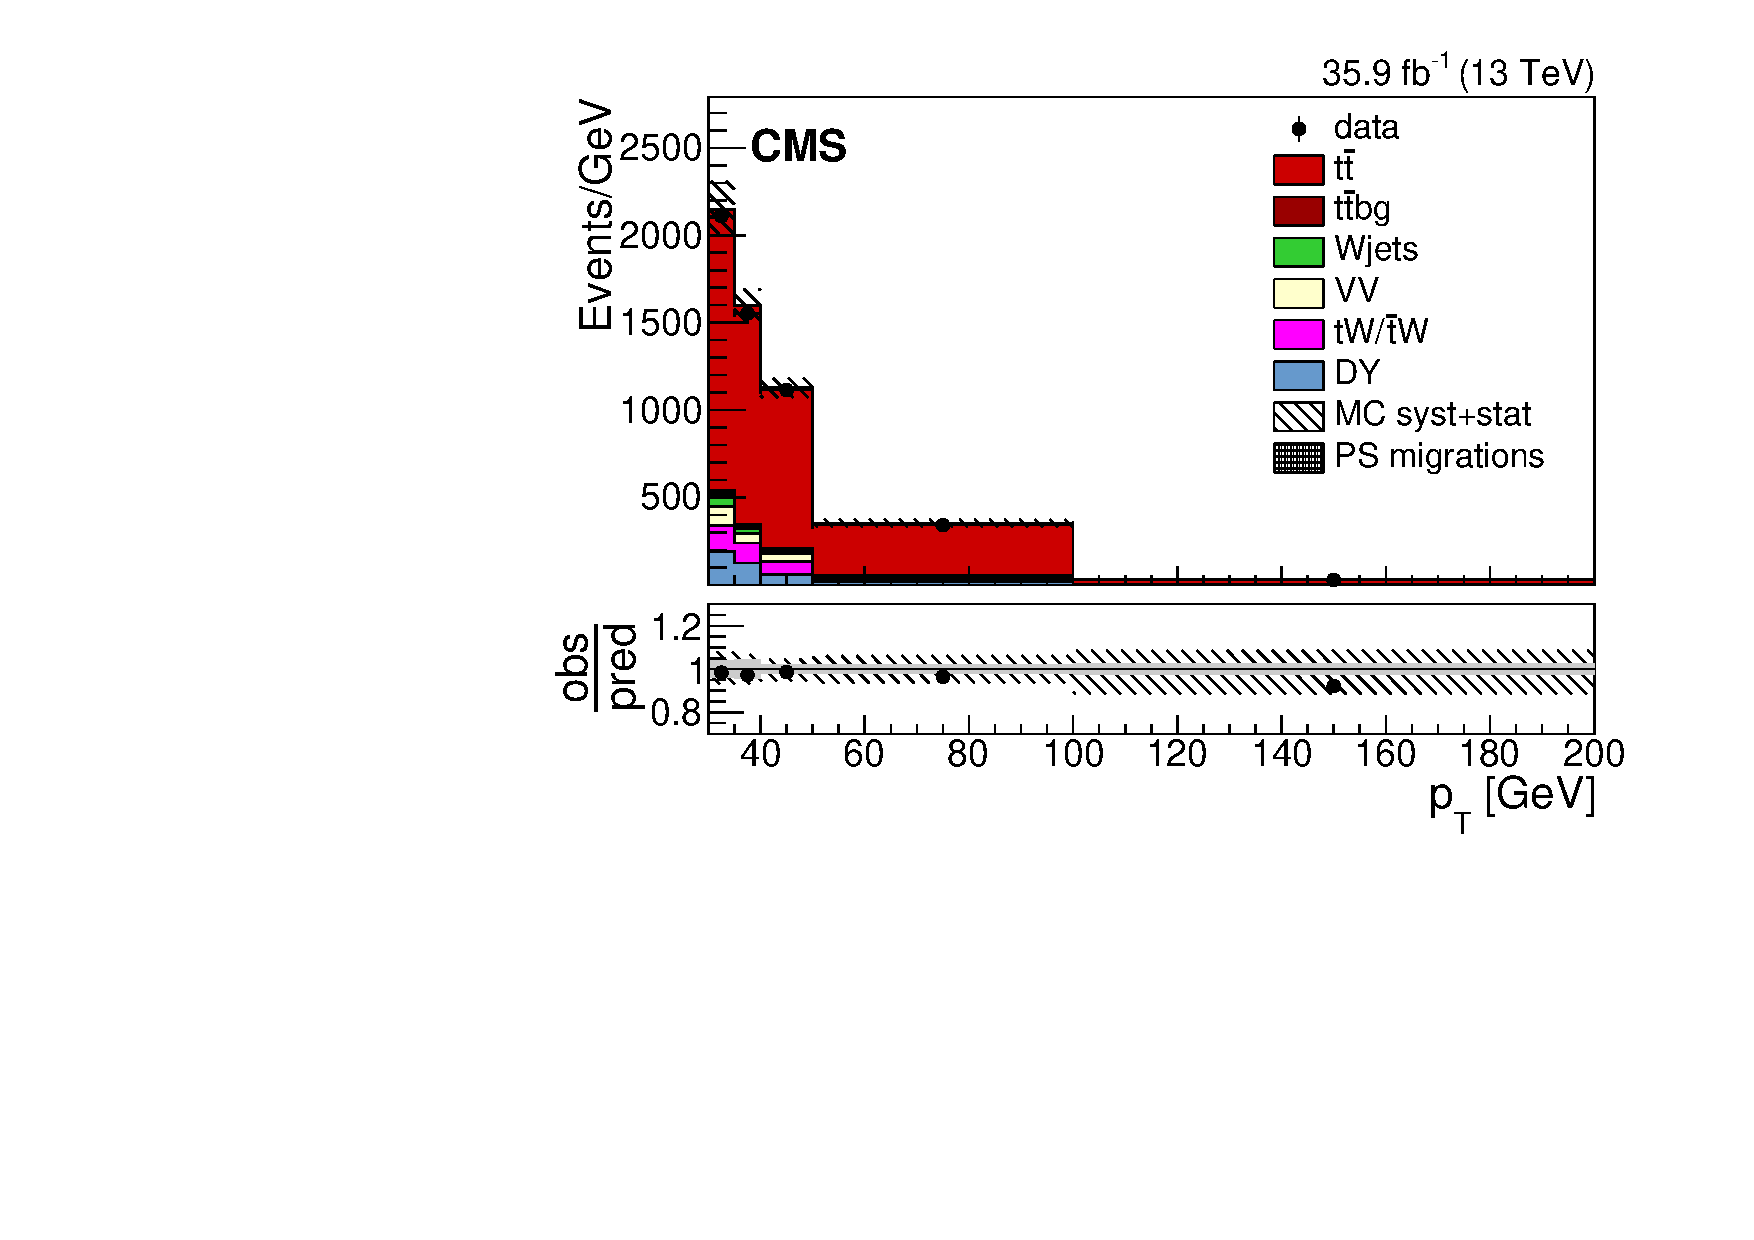
\includegraphics{CrossSection/Figures/ControlPlots/emu_sysnom/second_jet_pt_0_2_b-jets_step_8.pdf}}
    \resizebox{0.32 \textwidth}{!}{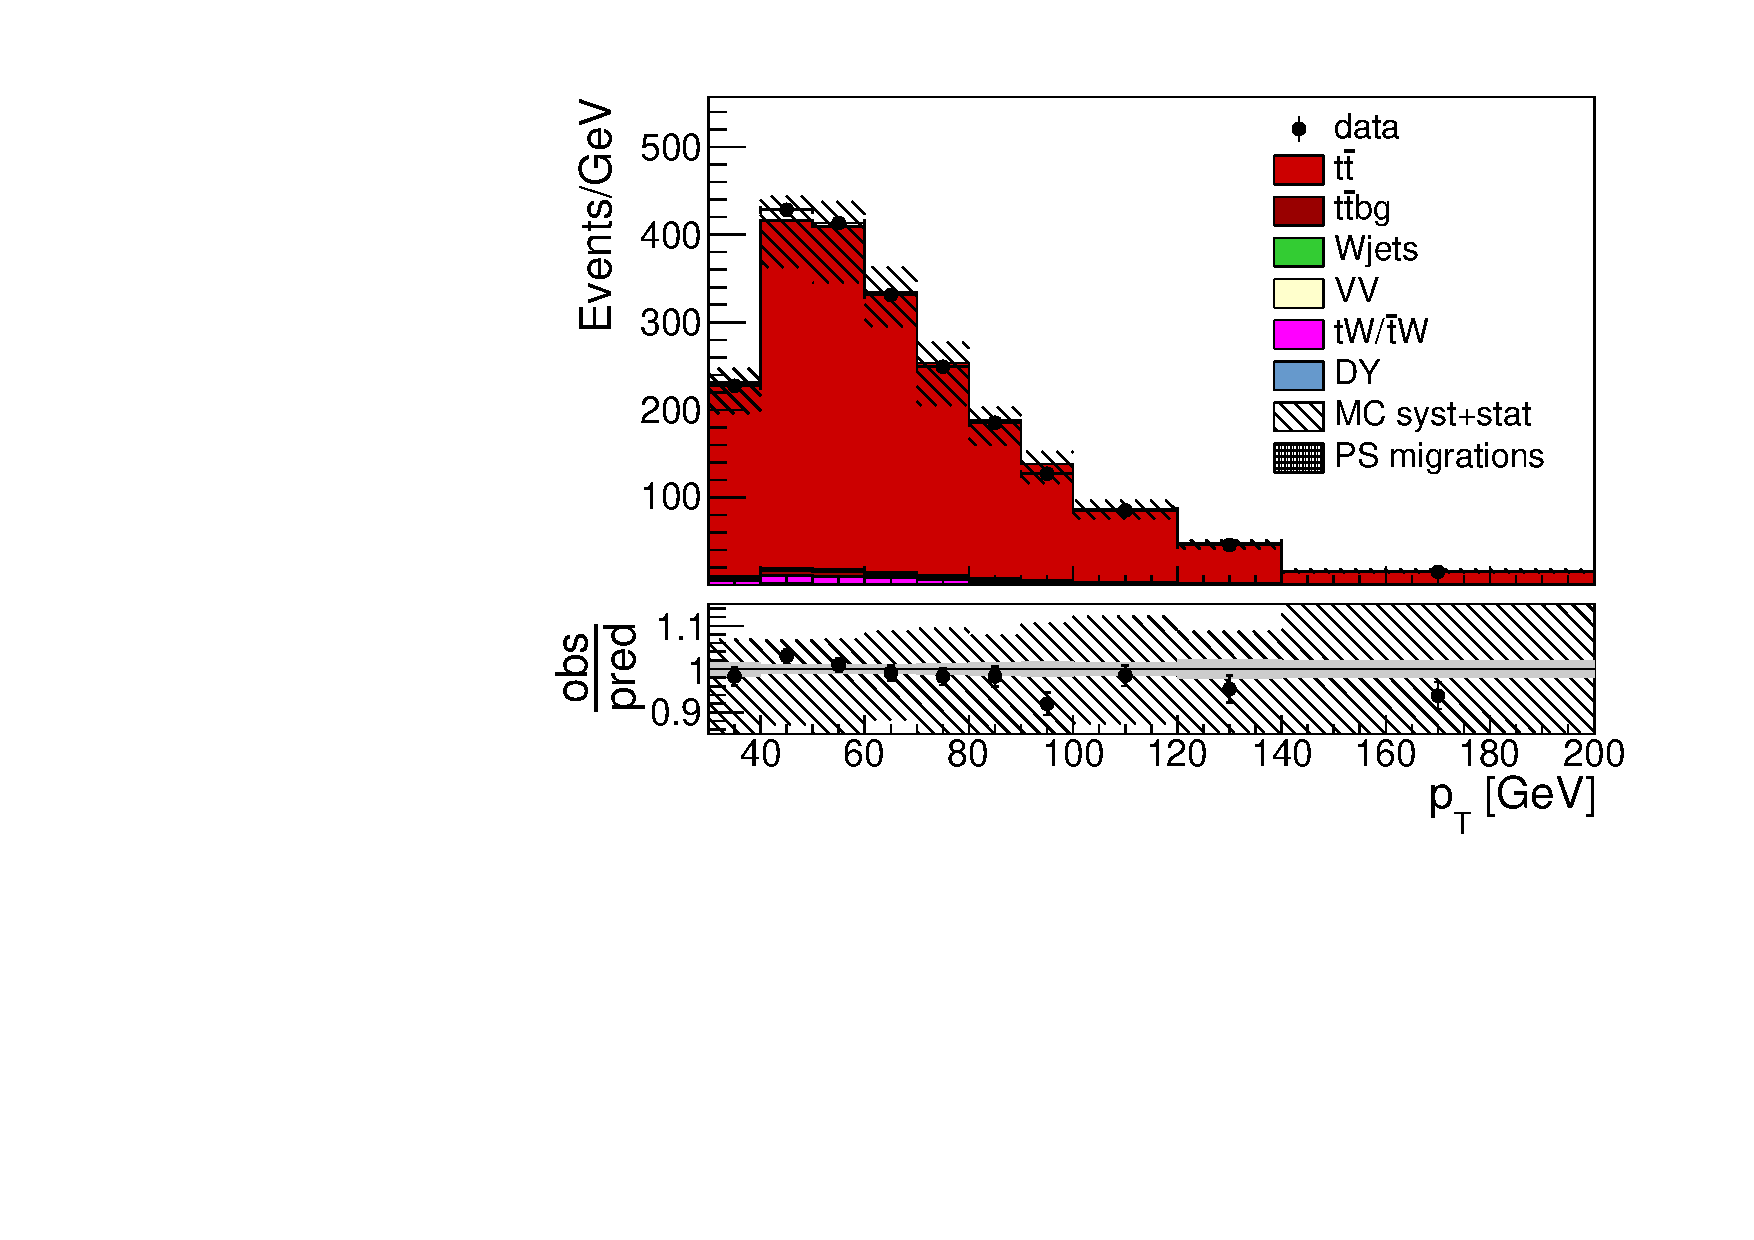
\includegraphics{CrossSection/Figures/ControlPlots/emu_sysnom/second_jet_pt_1_2_b-jets_step_8.pdf}}
    \resizebox{0.32 \textwidth}{!}{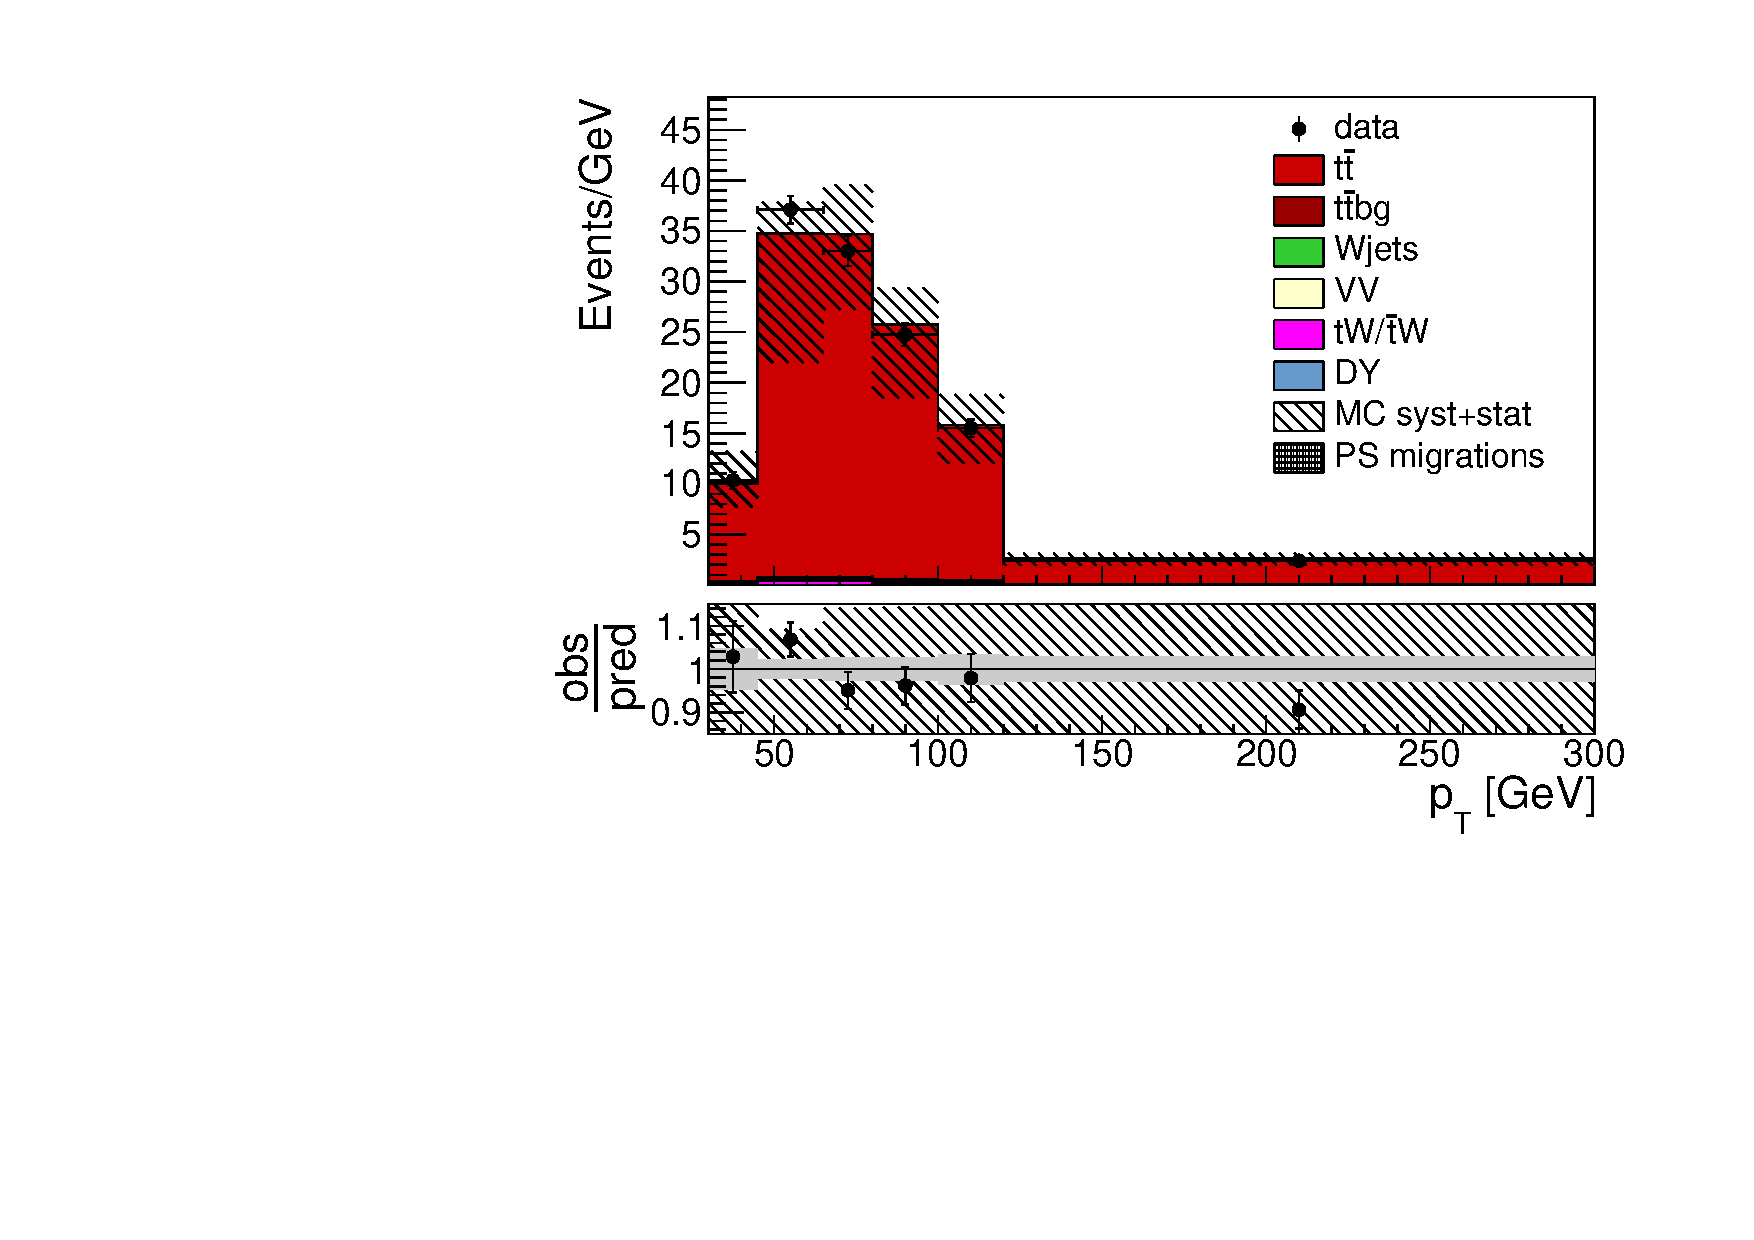
\includegraphics{CrossSection/Figures/ControlPlots/emu_sysnom/second_jet_pt_2_2_b-jets_step_8.pdf}}

    \resizebox{0.32 \textwidth}{!}{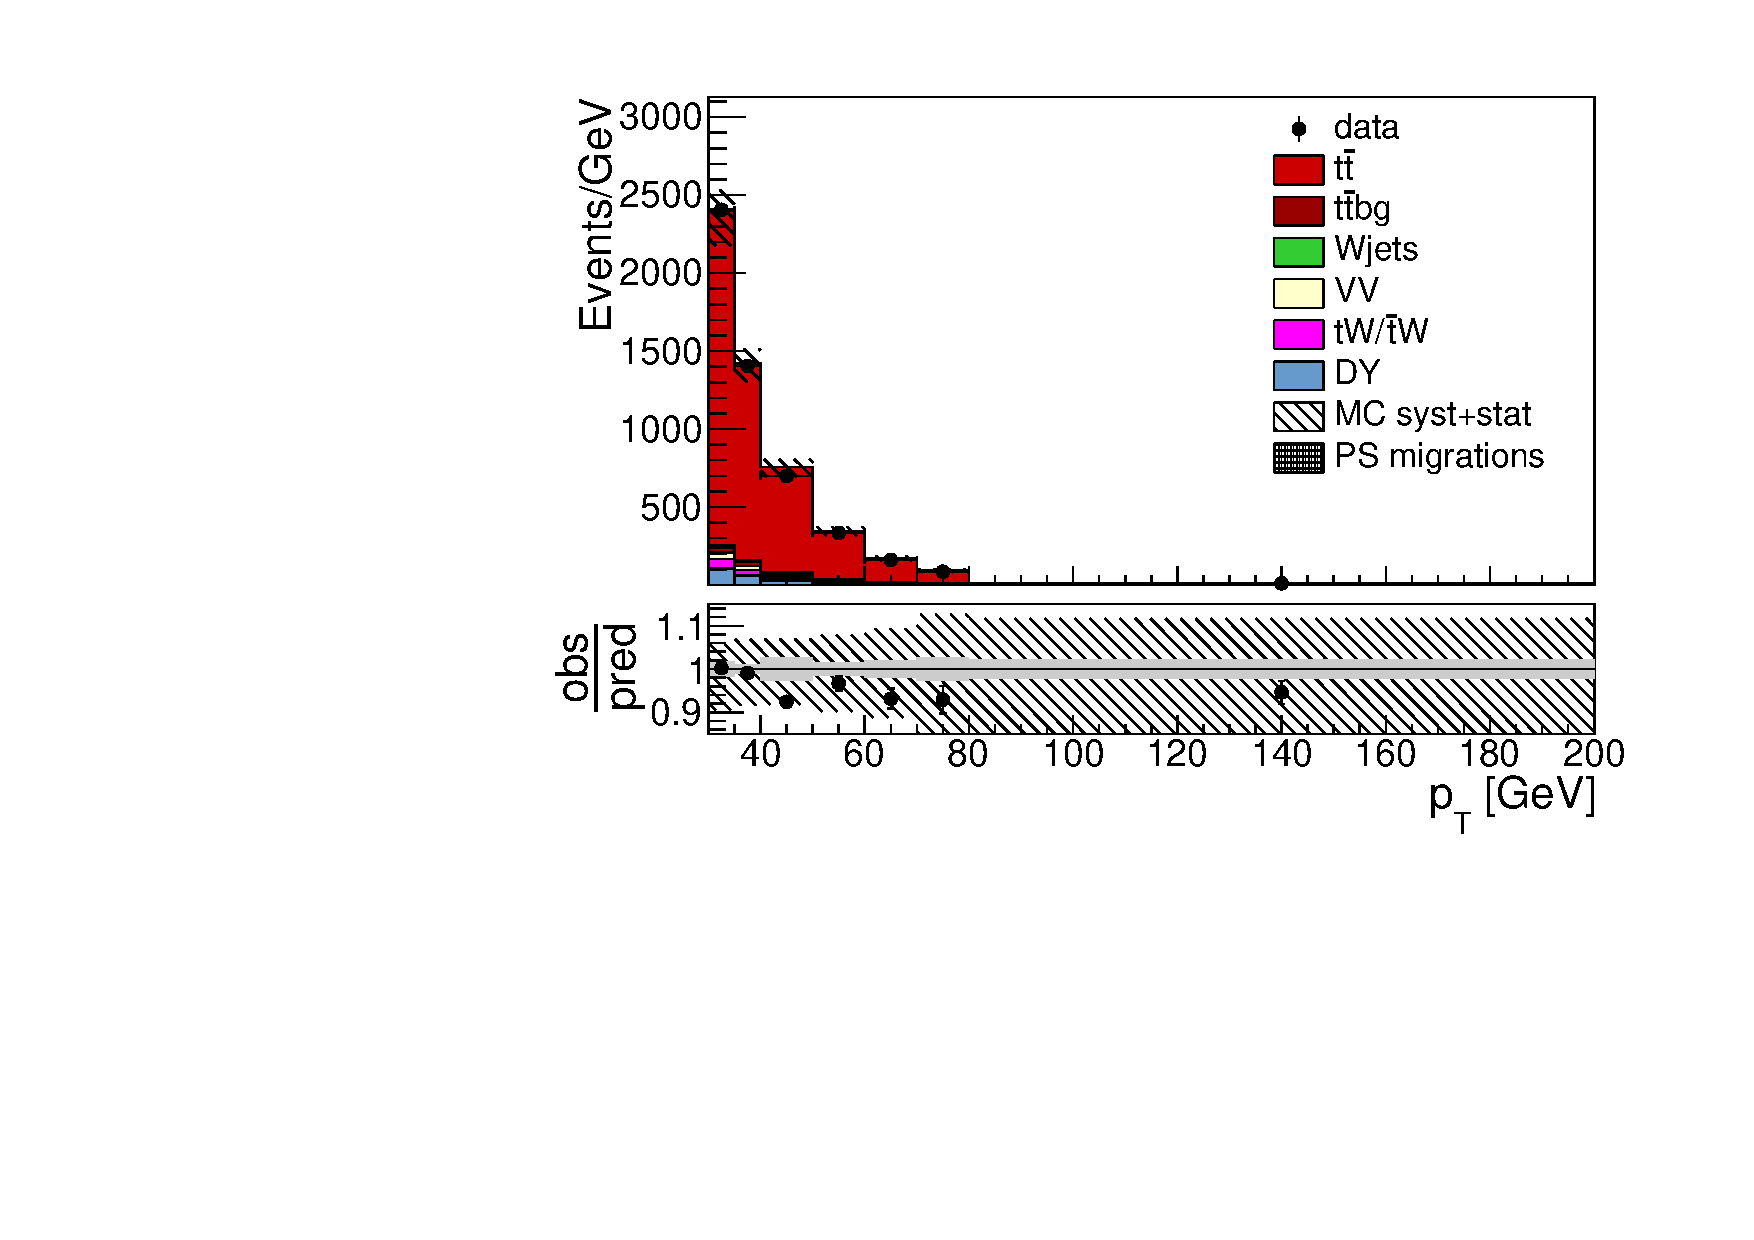
\includegraphics{CrossSection/Figures/ControlPlots/emu_sysnom/third_jet_pt_0_3_b-jets_step_8.pdf}}
    \resizebox{0.32 \textwidth}{!}{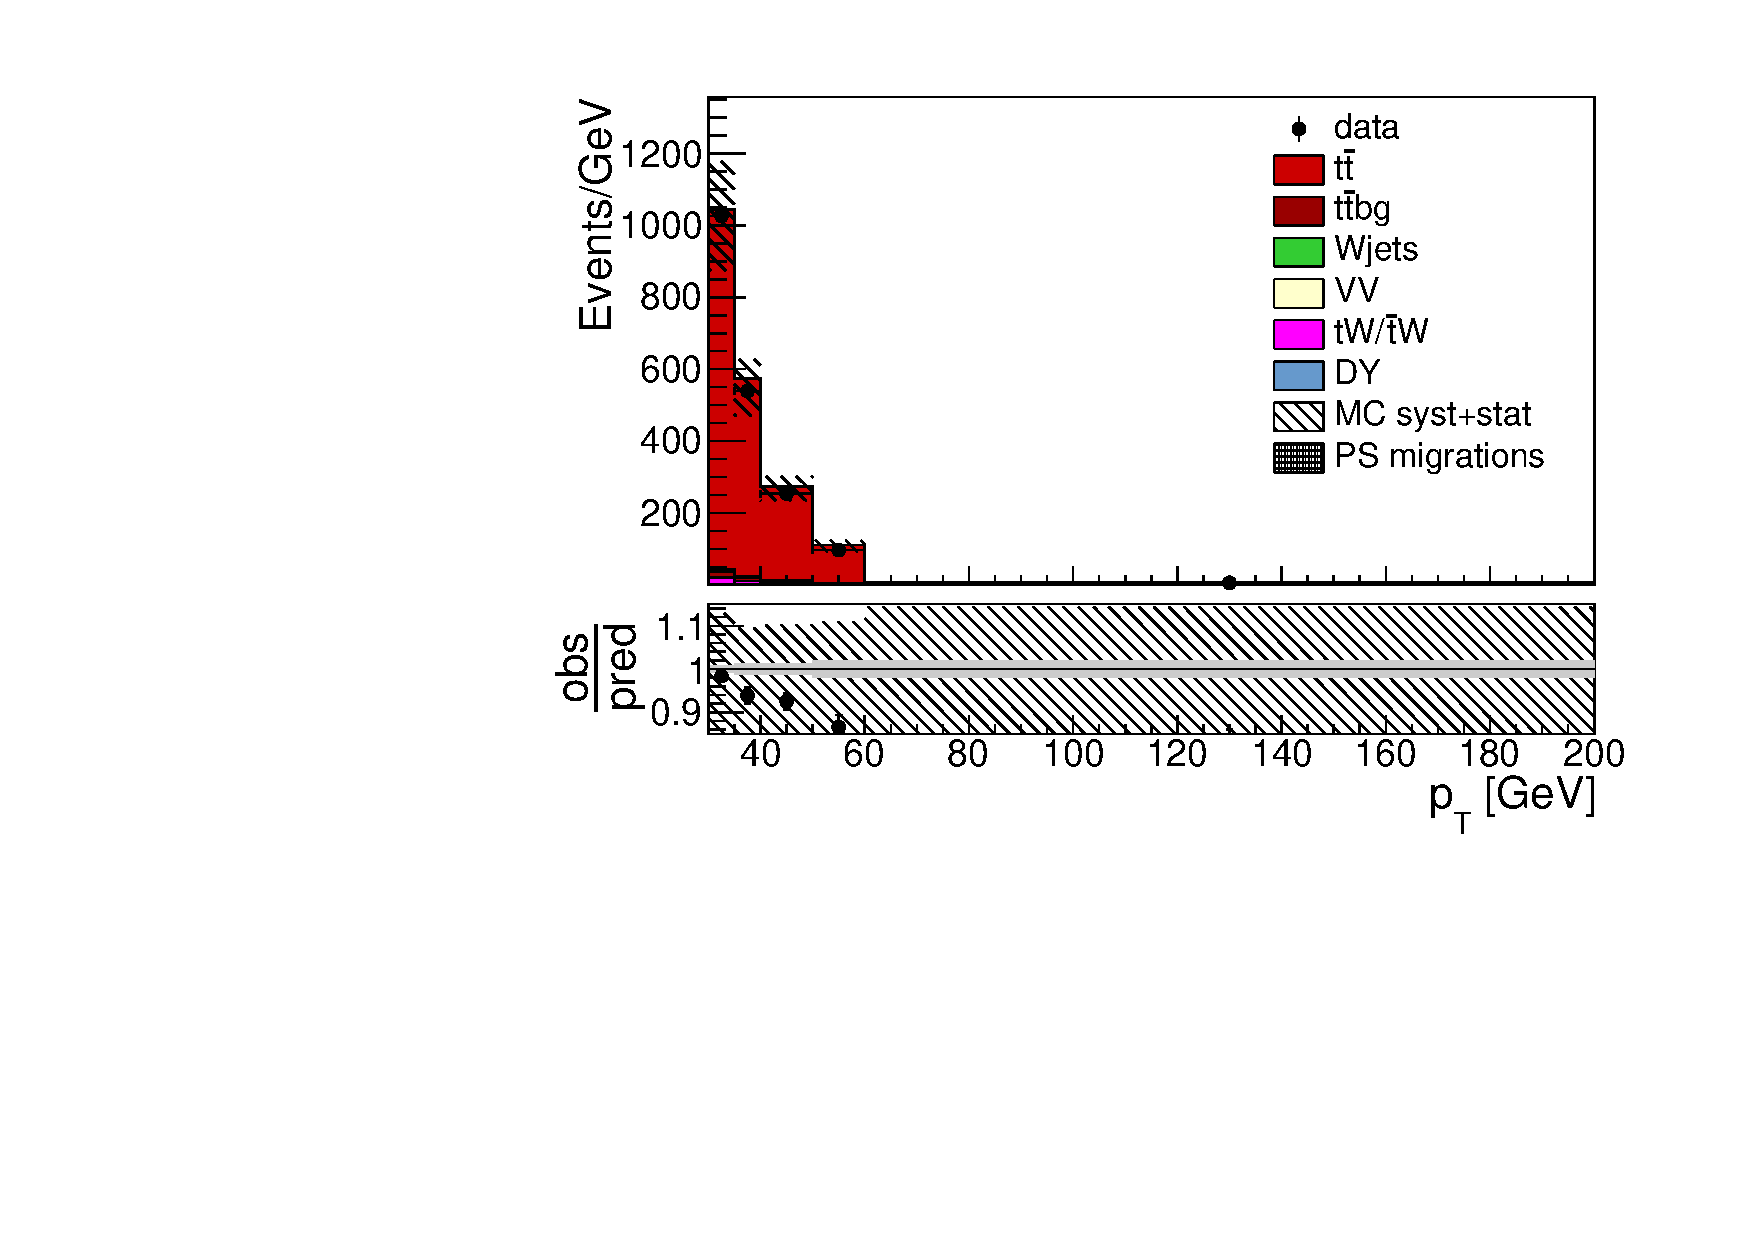
\includegraphics{CrossSection/Figures/ControlPlots/emu_sysnom/third_jet_pt_1_3_b-jets_step_8.pdf}}
    \resizebox{0.32 \textwidth}{!}{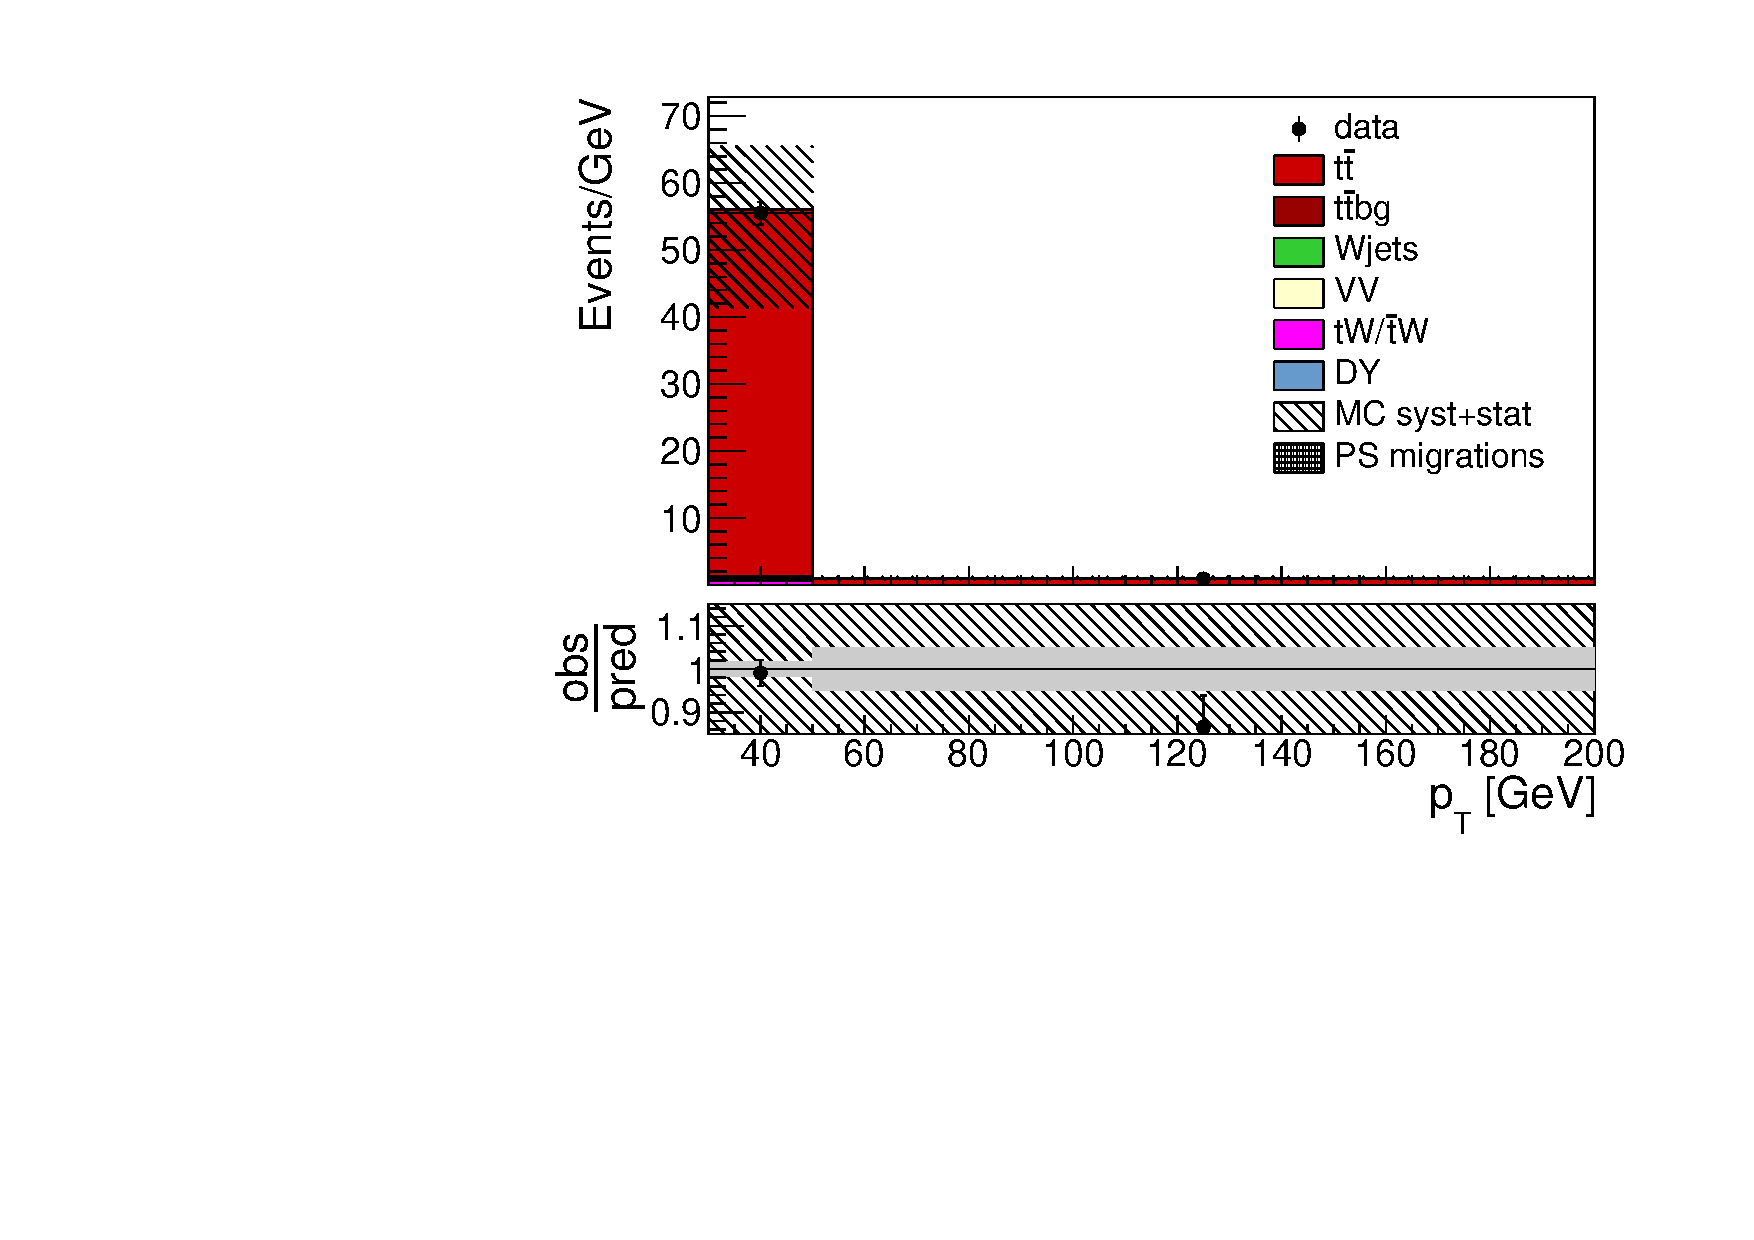
\includegraphics{CrossSection/Figures/ControlPlots/emu_sysnom/third_jet_pt_2_3_b-jets_step_8.pdf}}  

\caption{Template distributions for events in the \emu channel with zero as well as three or
  more b-tagged jets (left column), One b-tagged jet (middle column) or two b-tagged jets (right column). The distributions show the total event yield for zero (top) and the trailing jet pt for one (second from top),
  two (second from bottom) or three or more (bottom) additional jets. 
  The hatched bands correspond to the total uncertainty on the predicted number of events. The ratios of the event yields in data and the sum of the
  predicted yields are shown at the bottom of each plot. Here, the solid
  gray band represents the contribution of the statistical uncertainty.  
       \label{fig:xsec_emu_inputdistr}}
  \end{center}
\end{figure}

\begin{figure}[htbp!]
  \begin{center}
    \resizebox{0.40 \textwidth}{!}{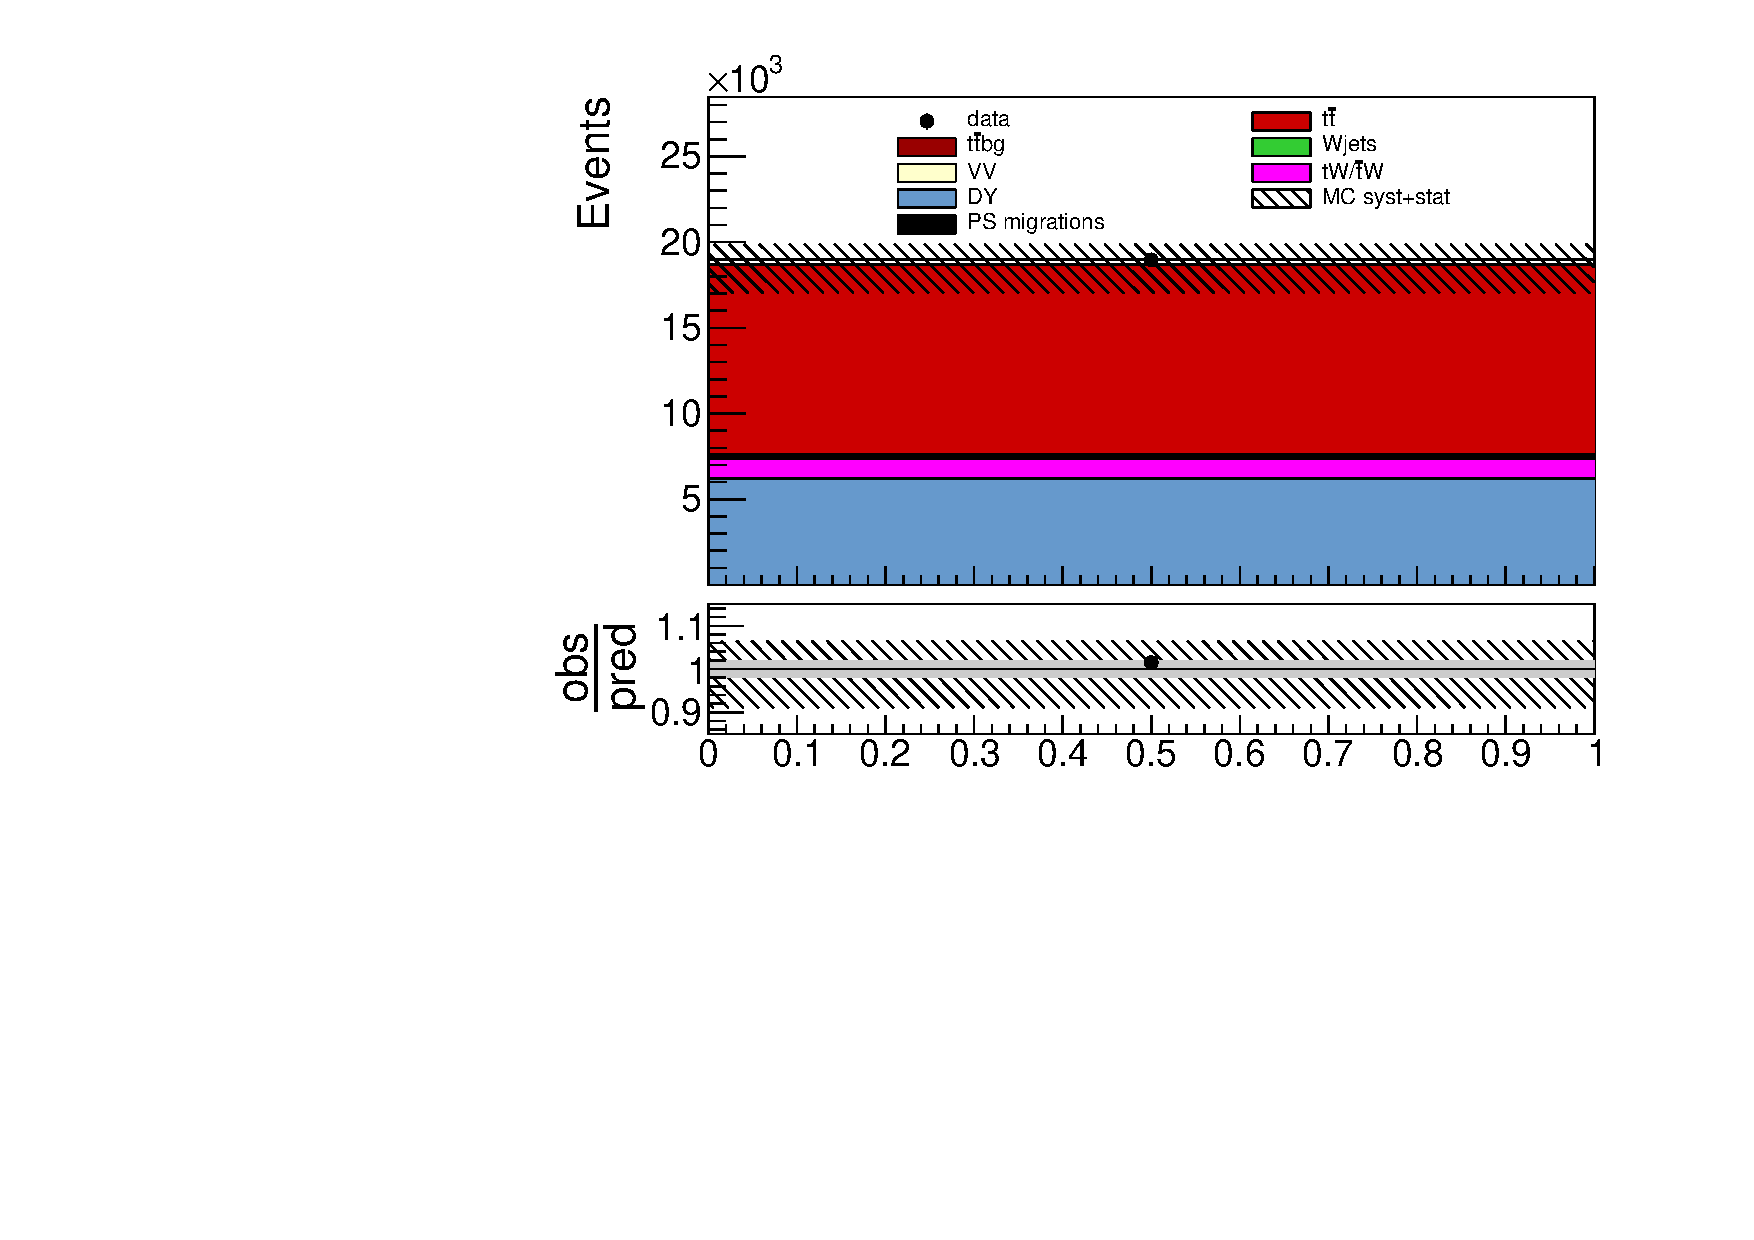
\includegraphics{CrossSection/Figures/ControlPlots/mumu_sysnom/total_1_0_b-jets_step_8.pdf}}
    \resizebox{0.40 \textwidth}{!}{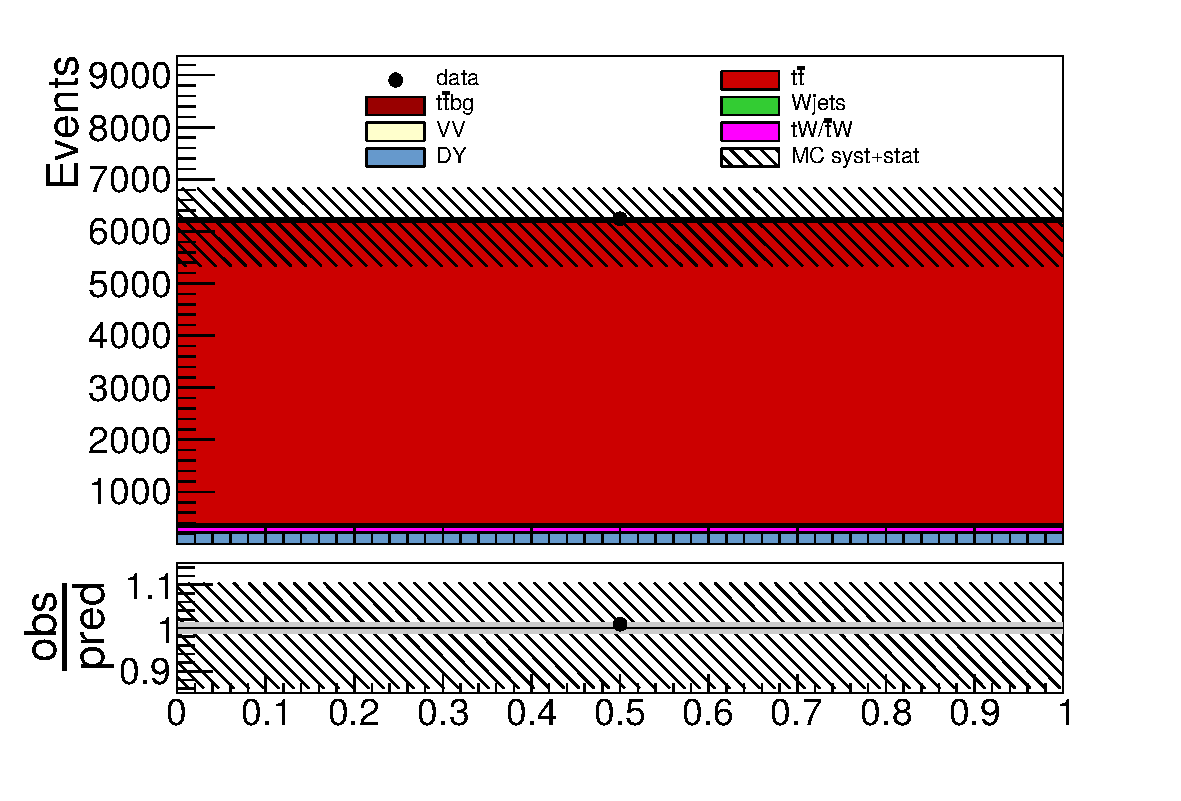
\includegraphics{CrossSection/Figures/ControlPlots/mumu_sysnom/total_2_0_b-jets_step_8.pdf}} \\

    \resizebox{0.40 \textwidth}{!}{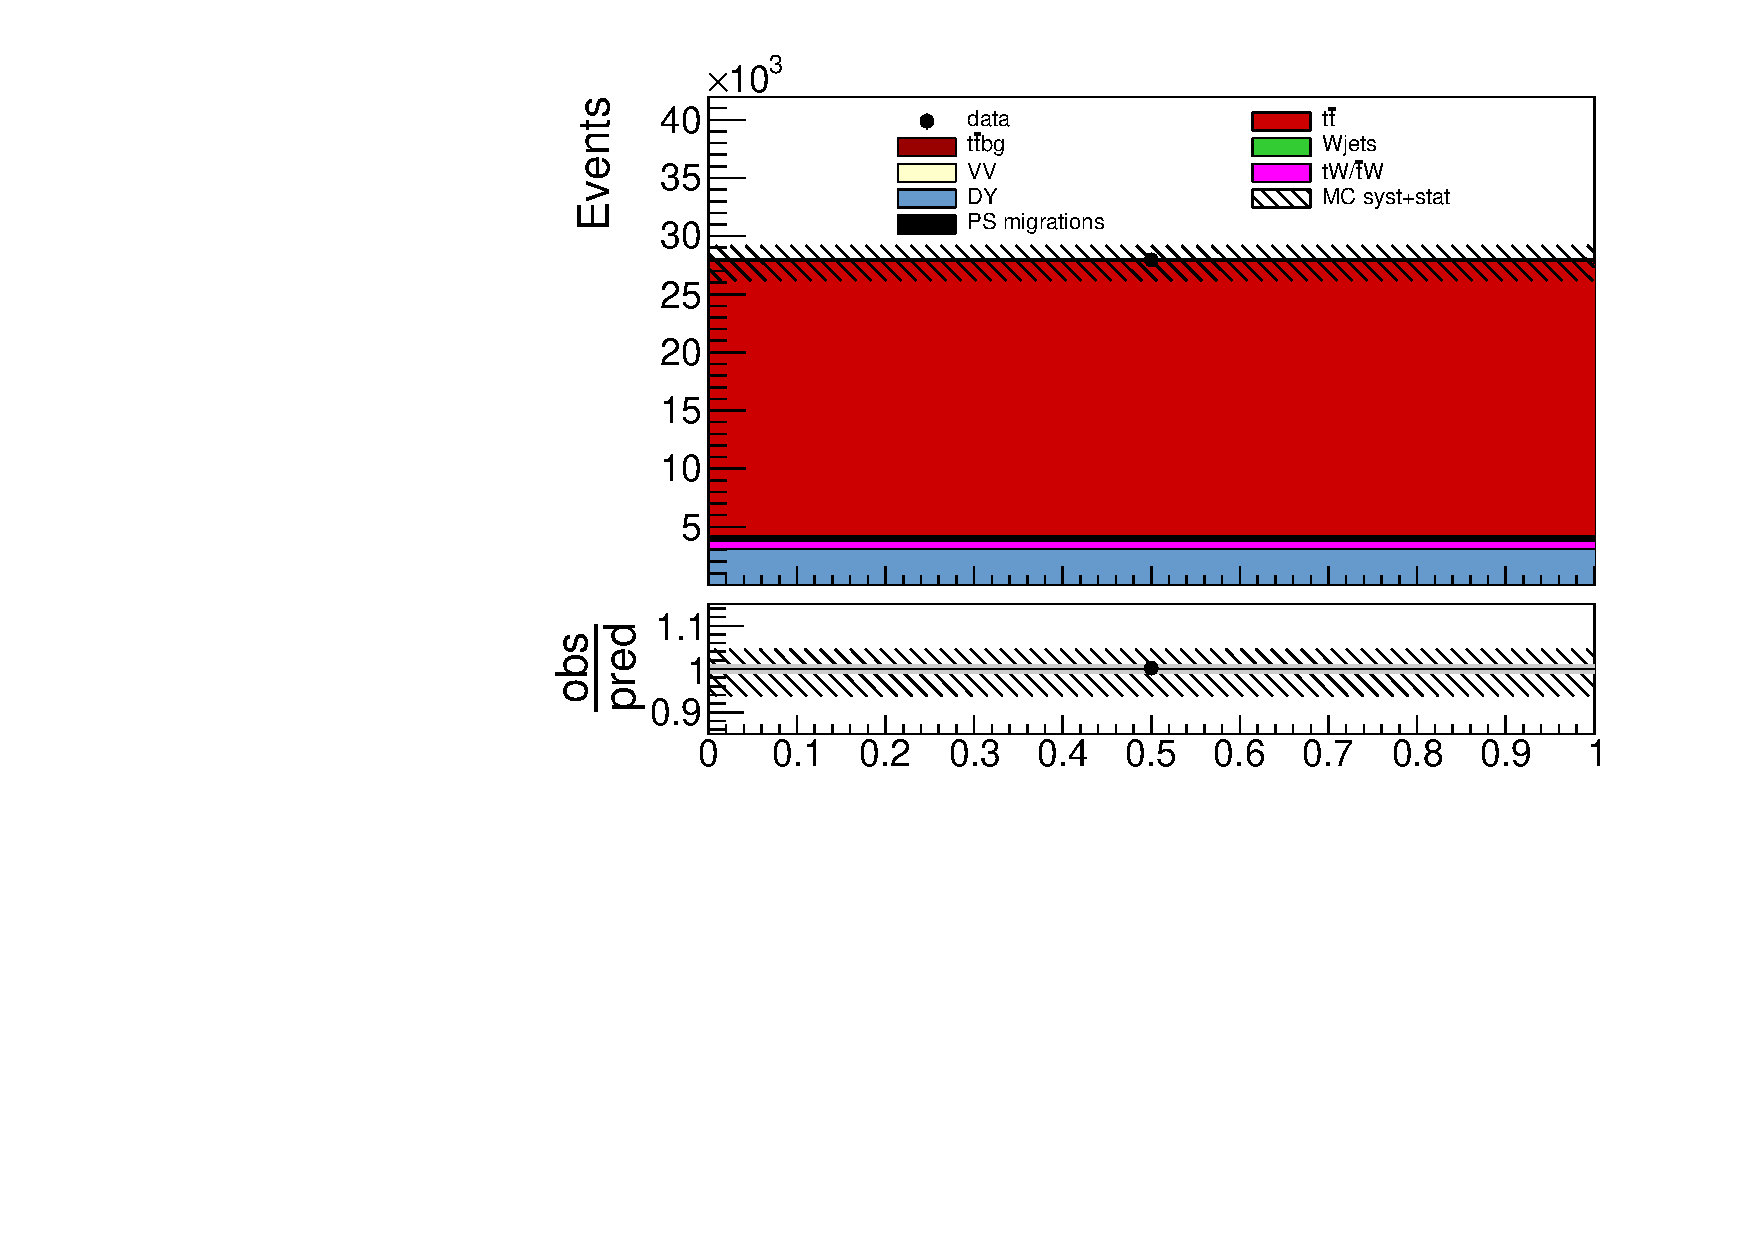
\includegraphics{CrossSection/Figures/ControlPlots/mumu_sysnom/total_1_1_b-jets_step_8.pdf}}
    \resizebox{0.40 \textwidth}{!}{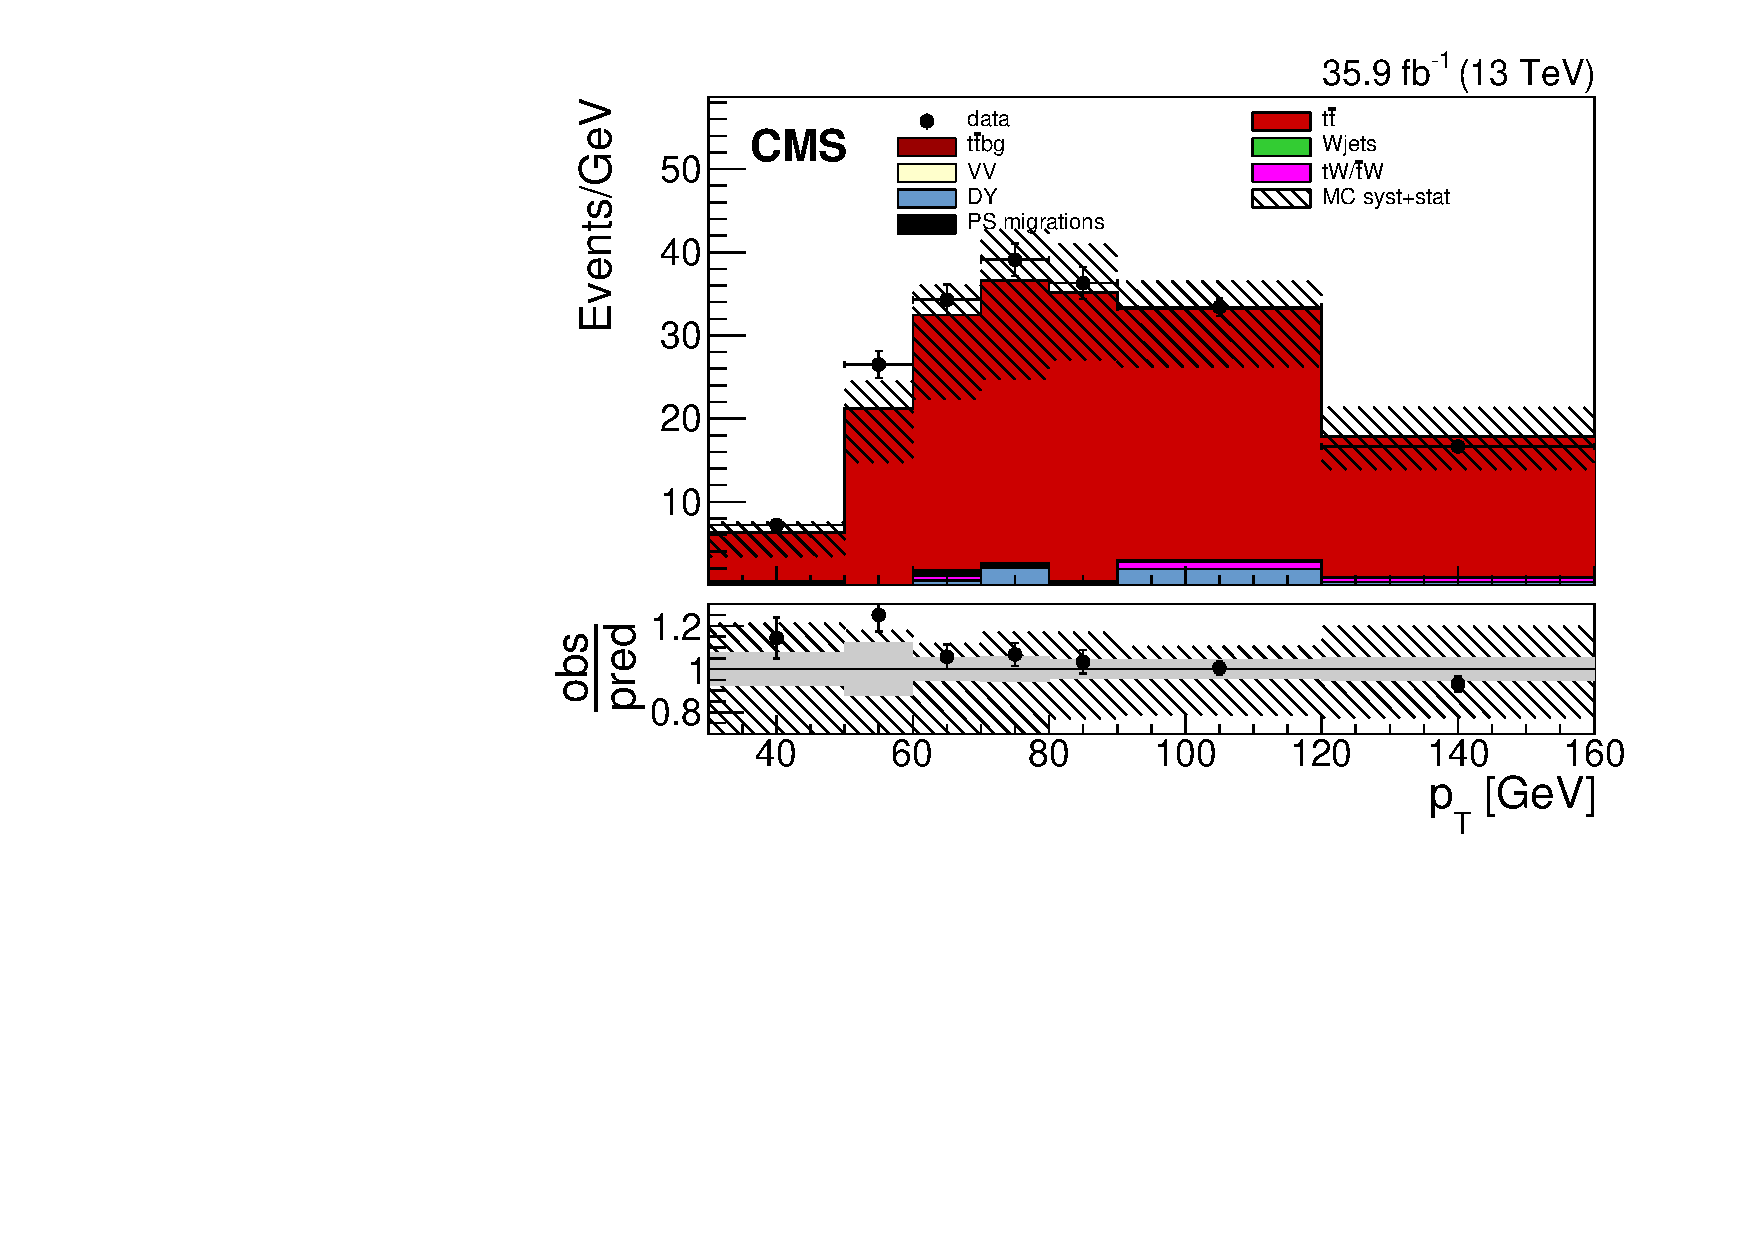
\includegraphics{CrossSection/Figures/ControlPlots/mumu_sysnom/lead_jet_pt_2_1_b-jets_step_8.pdf}}\\
        
    \resizebox{0.4 \textwidth}{!}{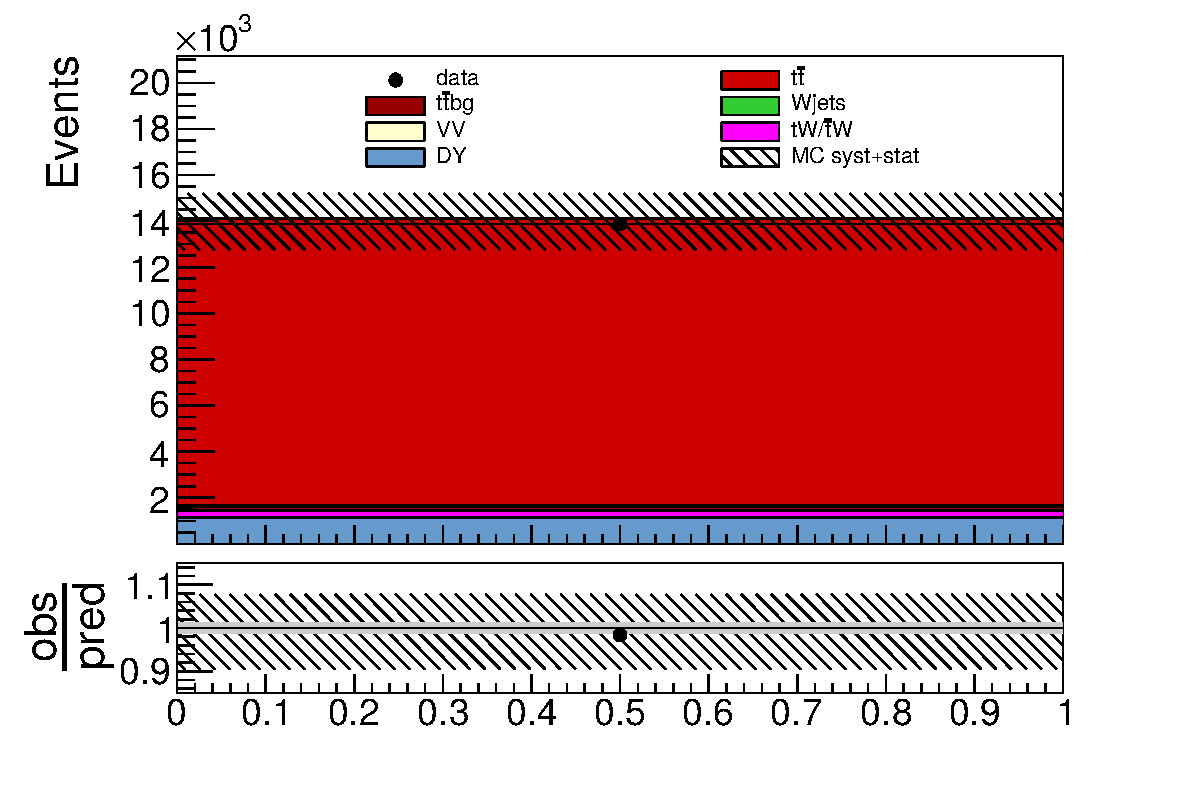
\includegraphics{CrossSection/Figures/ControlPlots/mumu_sysnom/total_1_2_b-jets_step_8.pdf}}
    \resizebox{0.4 \textwidth}{!}{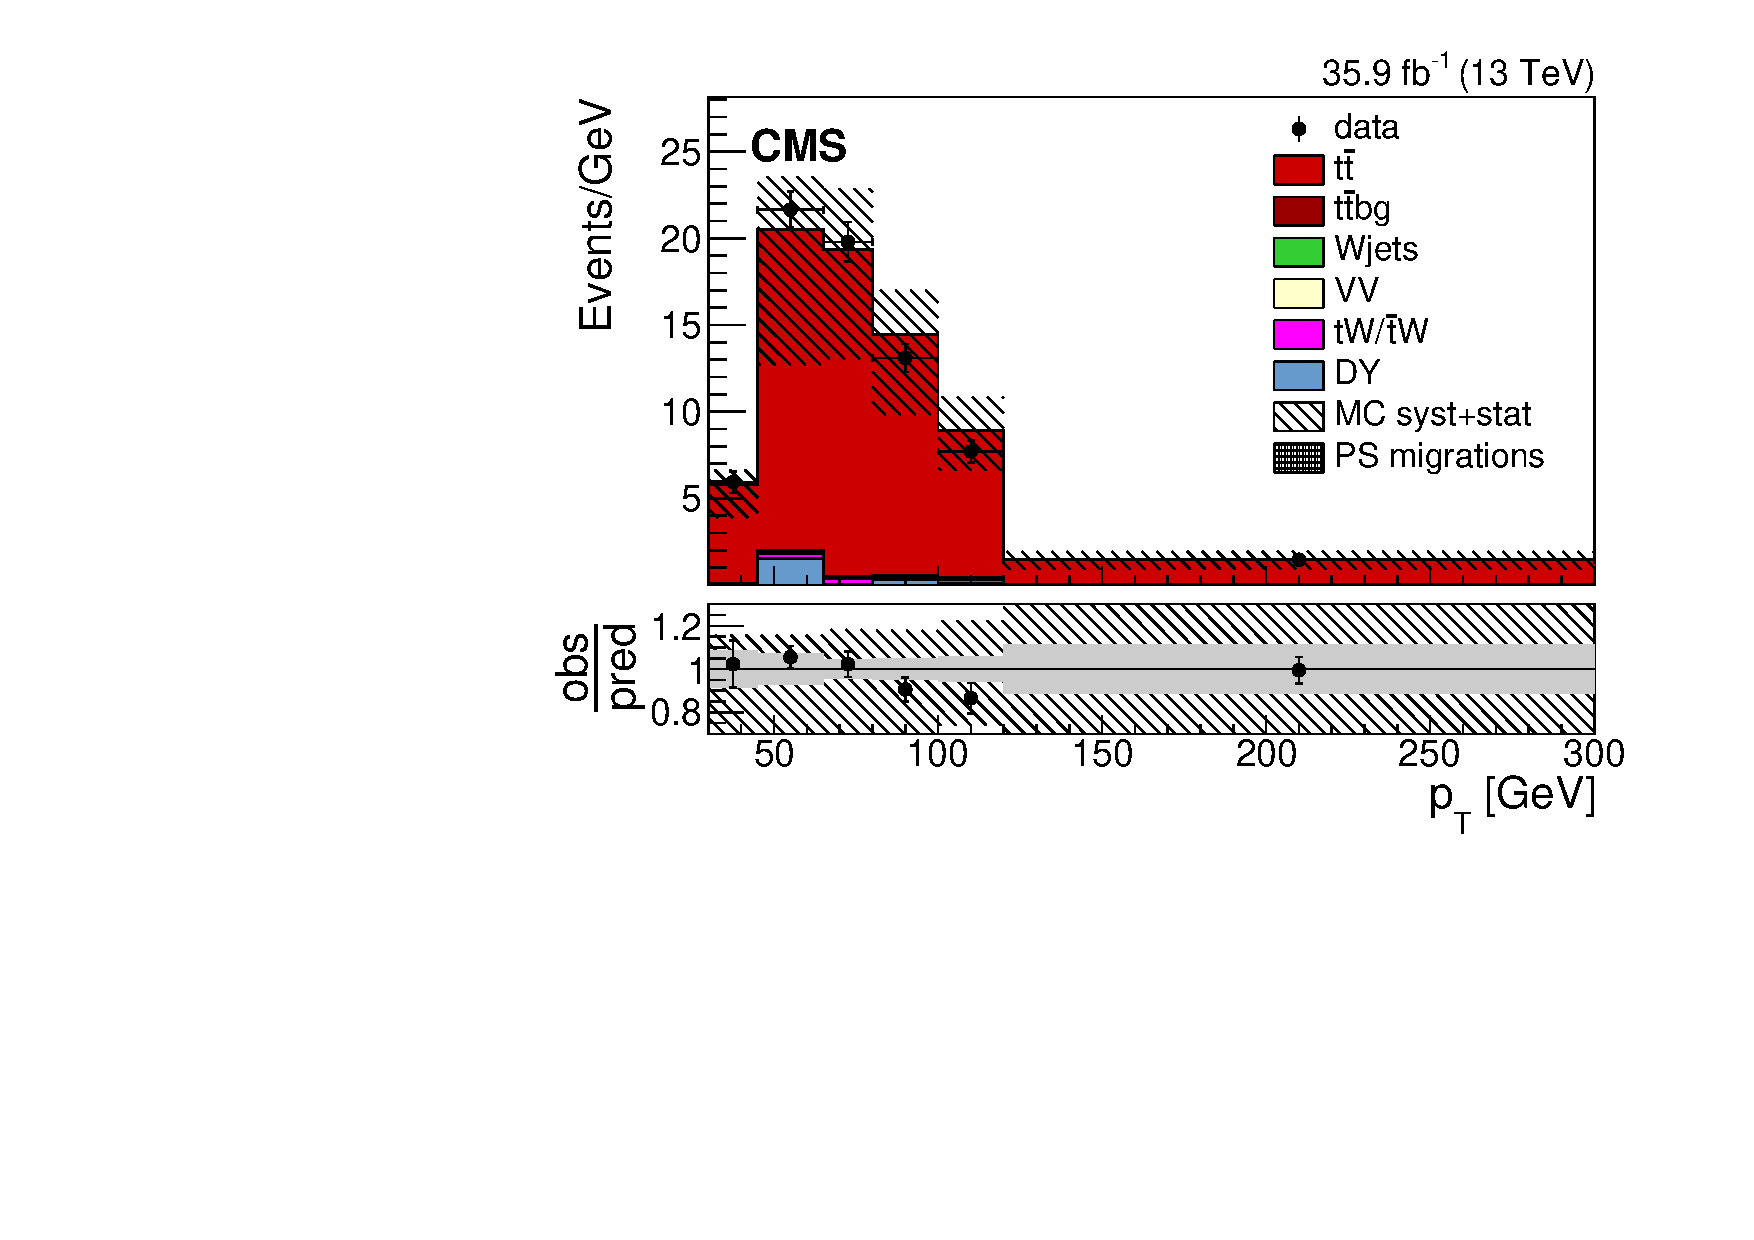
\includegraphics{CrossSection/Figures/ControlPlots/mumu_sysnom/second_jet_pt_2_2_b-jets_step_8.pdf}}\\

    \resizebox{0.4 \textwidth}{!}{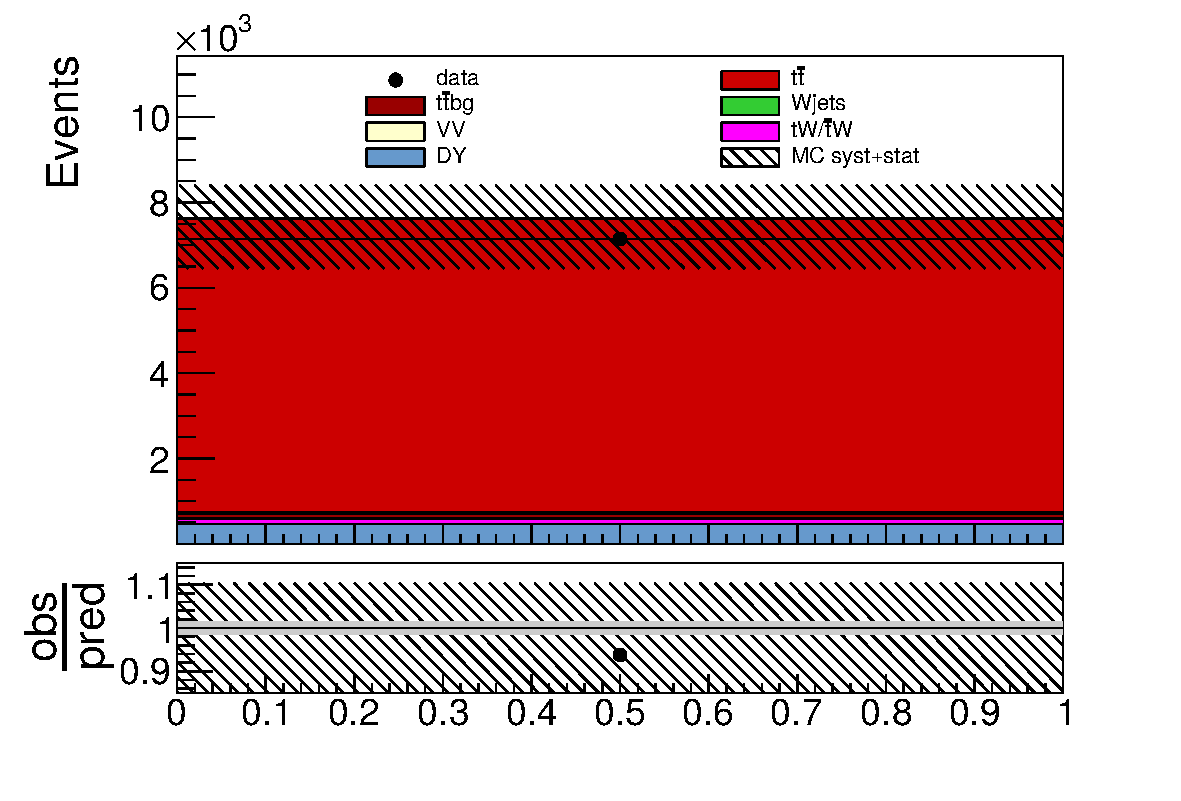
\includegraphics{CrossSection/Figures/ControlPlots/mumu_sysnom/total_1_3_b-jets_step_8.pdf}}
    \resizebox{0.4 \textwidth}{!}{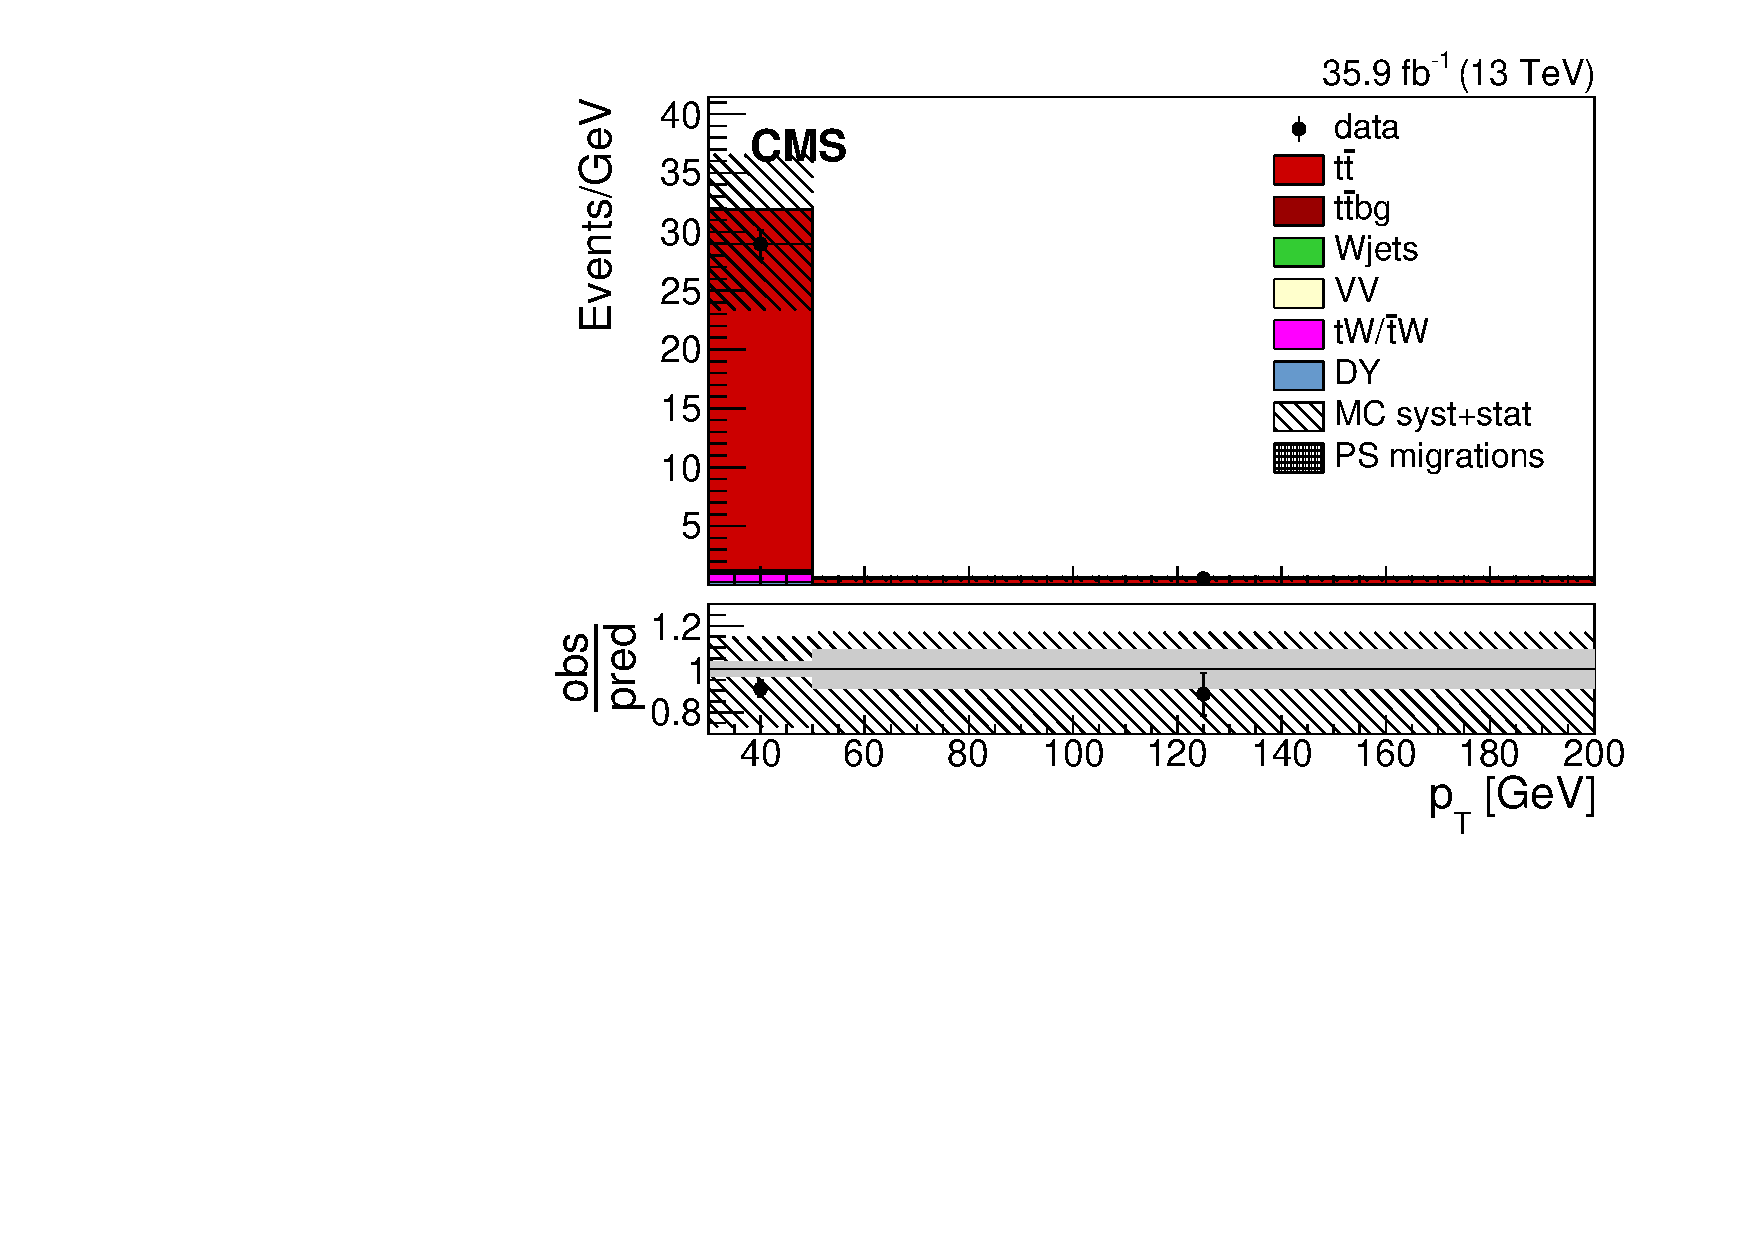
\includegraphics{CrossSection/Figures/ControlPlots/mumu_sysnom/third_jet_pt_2_3_b-jets_step_8.pdf}}  
\caption{Template distributions for events in the \mumu channel with one b-tagged jet (left column) or two b-tagged jets (right column). The distributions show the total event yield for zero (top) nd the trailing jet pt for one (second from top),
  two (second from bottom) or three or more (bottom) additional jets. 
  The hatched bands correspond to the total uncertainty on the predicted number of events. The ratios of the event yields in data and the sum of the
  predicted yields are shown at the bottom of each plot. Here, the solid
  gray band represents the contribution of the statistical uncertainty.  
       \label{fig:xsec_mumu_inputdistr}}
  \end{center}
\end{figure}

\begin{figure}[htbp!]
  \begin{center}
    \resizebox{0.4 \textwidth}{!}{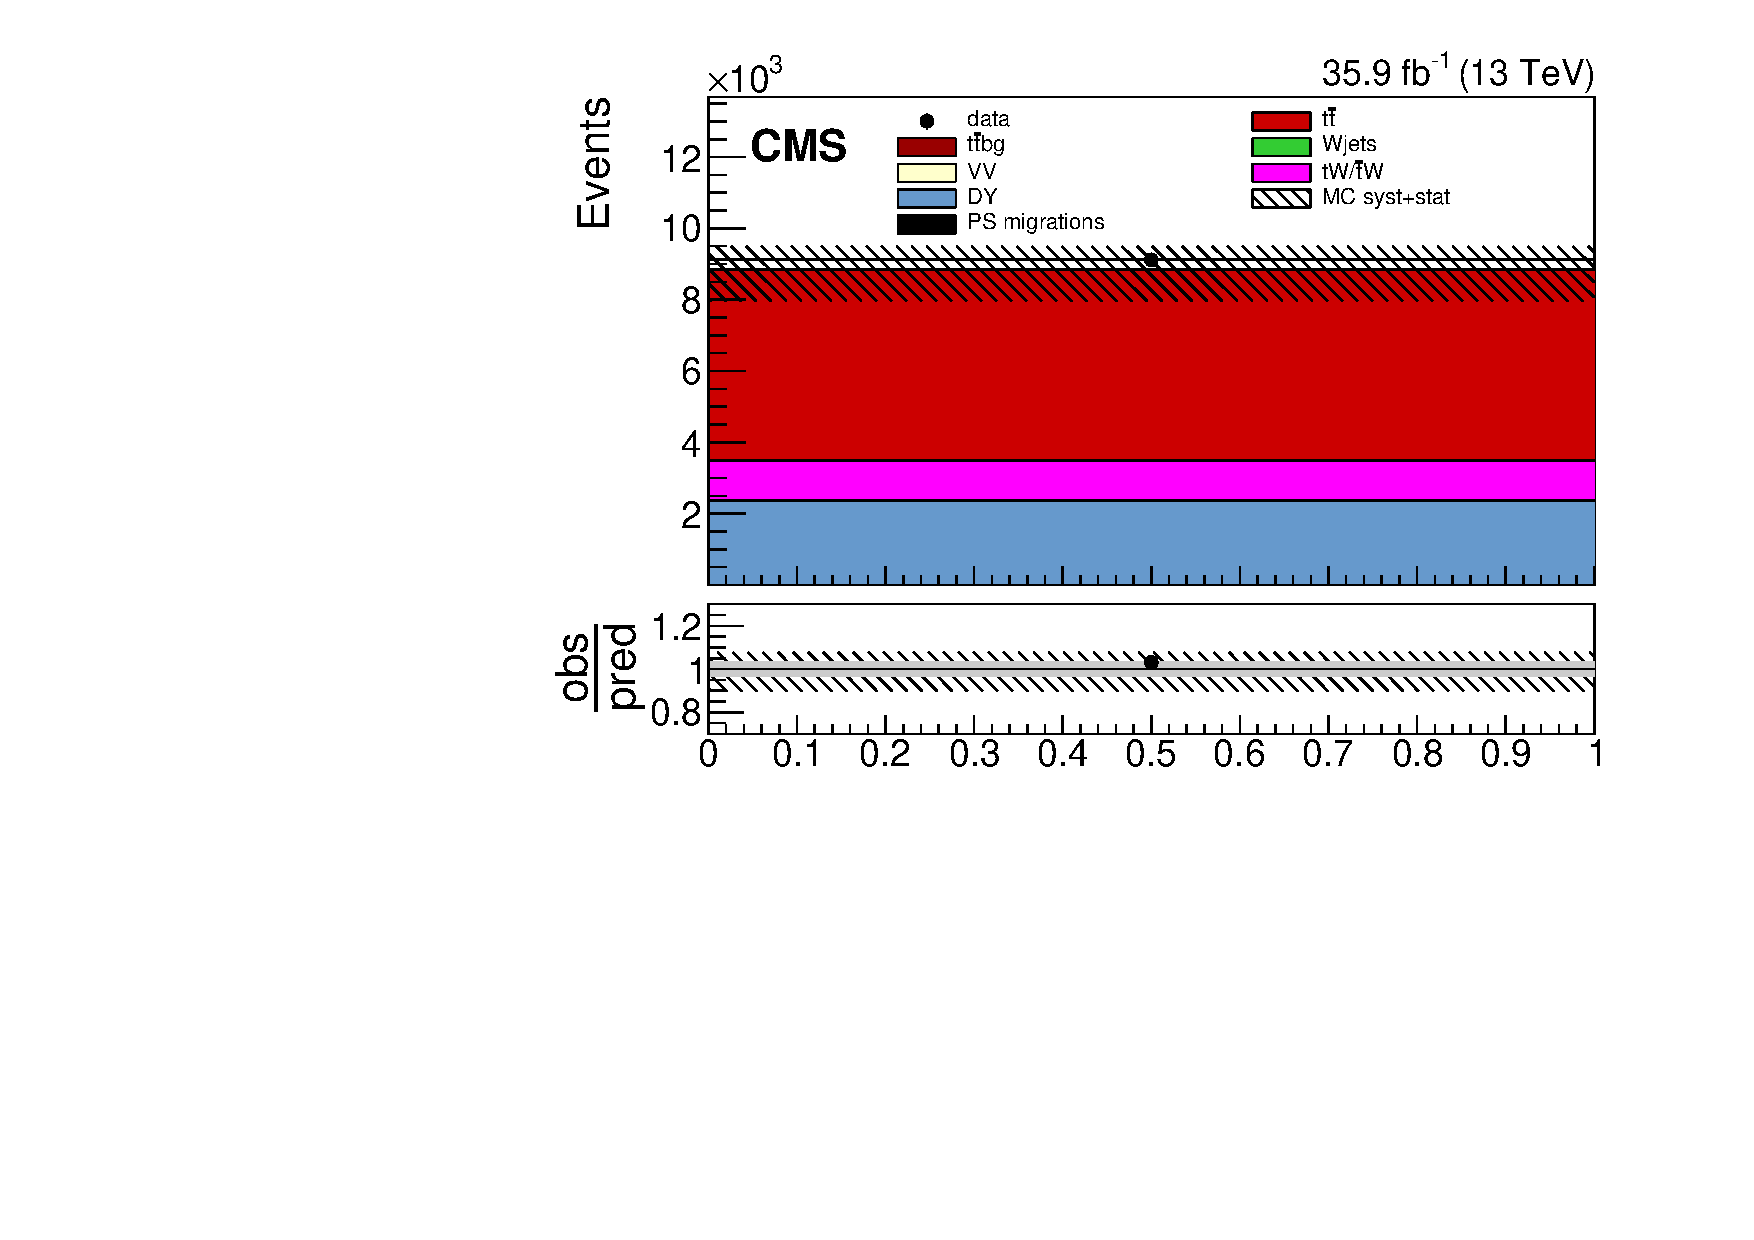
\includegraphics{CrossSection/Figures/ControlPlots/ee_sysnom/total_1_0_b-jets_step_8.pdf}}
    \resizebox{0.4 \textwidth}{!}{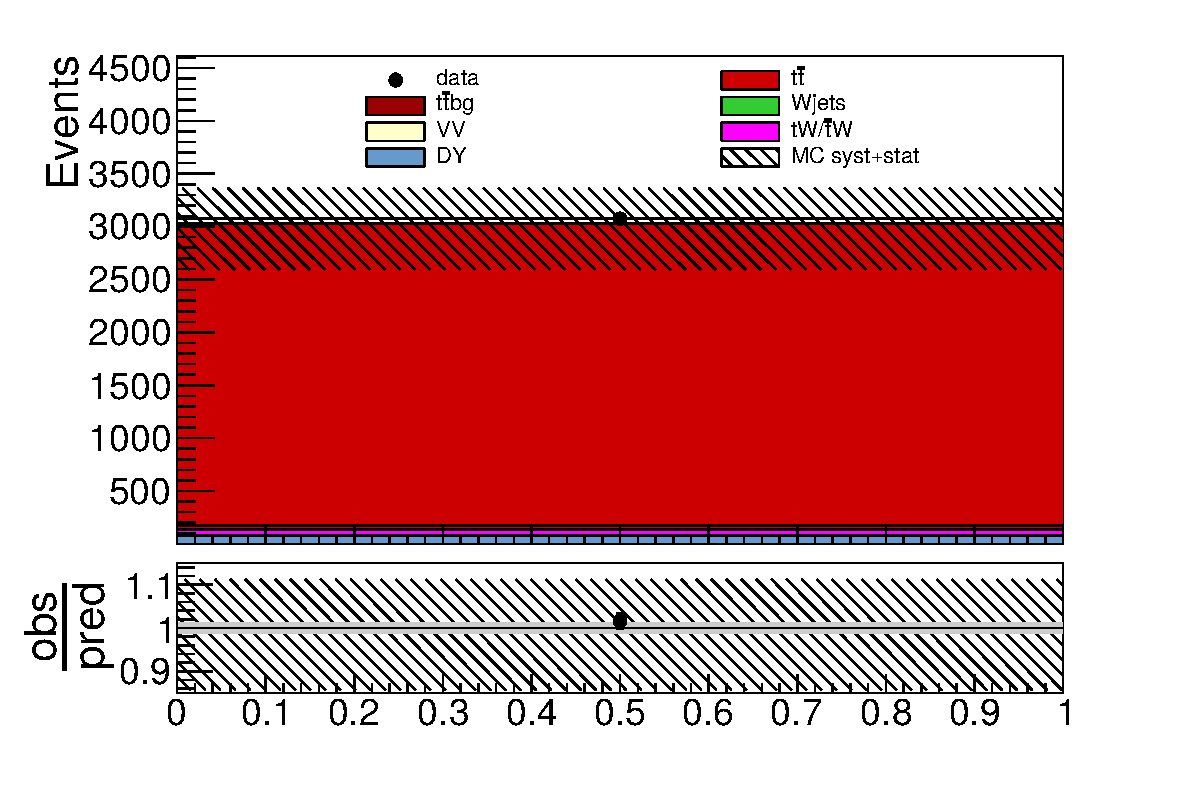
\includegraphics{CrossSection/Figures/ControlPlots/ee_sysnom/total_2_0_b-jets_step_8.pdf}}\\

    \resizebox{0.4 \textwidth}{!}{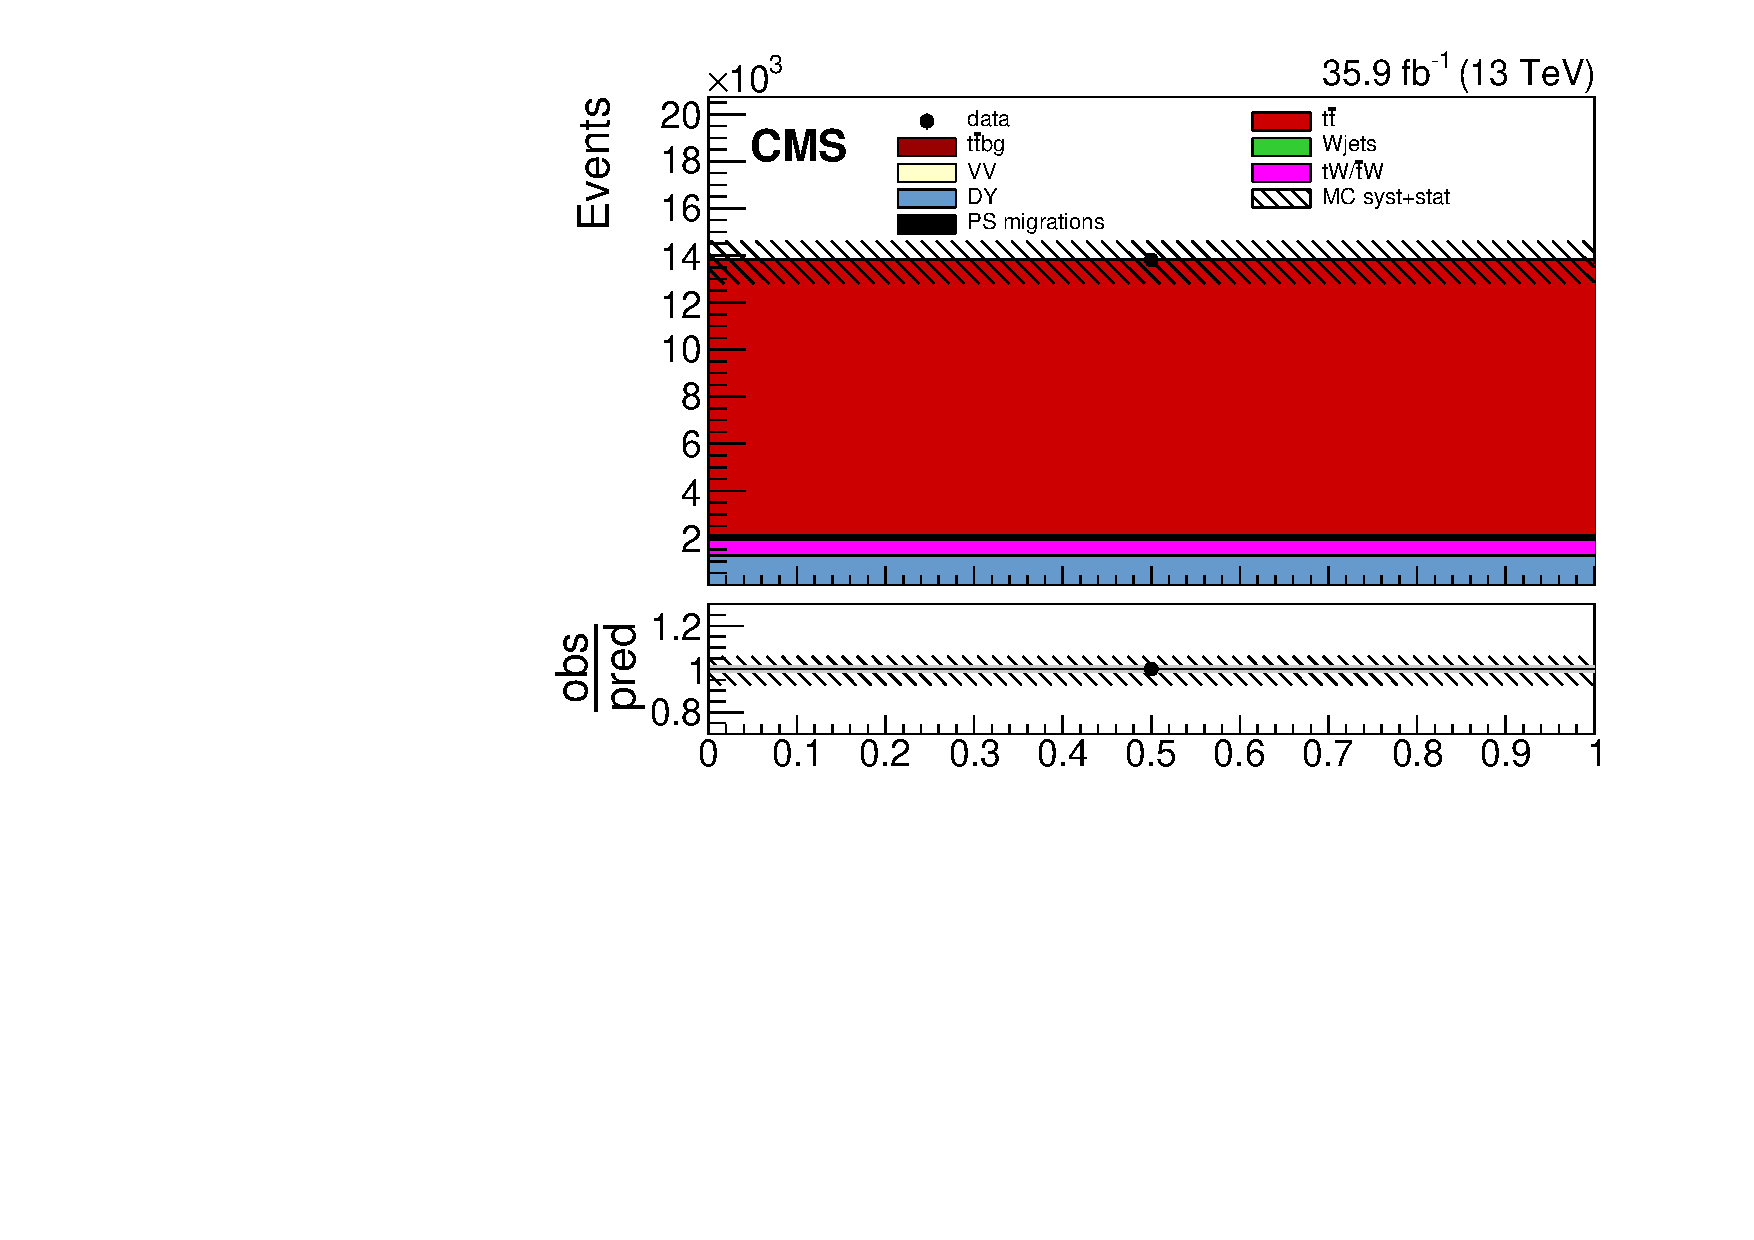
\includegraphics{CrossSection/Figures/ControlPlots/ee_sysnom/total_1_1_b-jets_step_8.pdf}}
    \resizebox{0.4 \textwidth}{!}{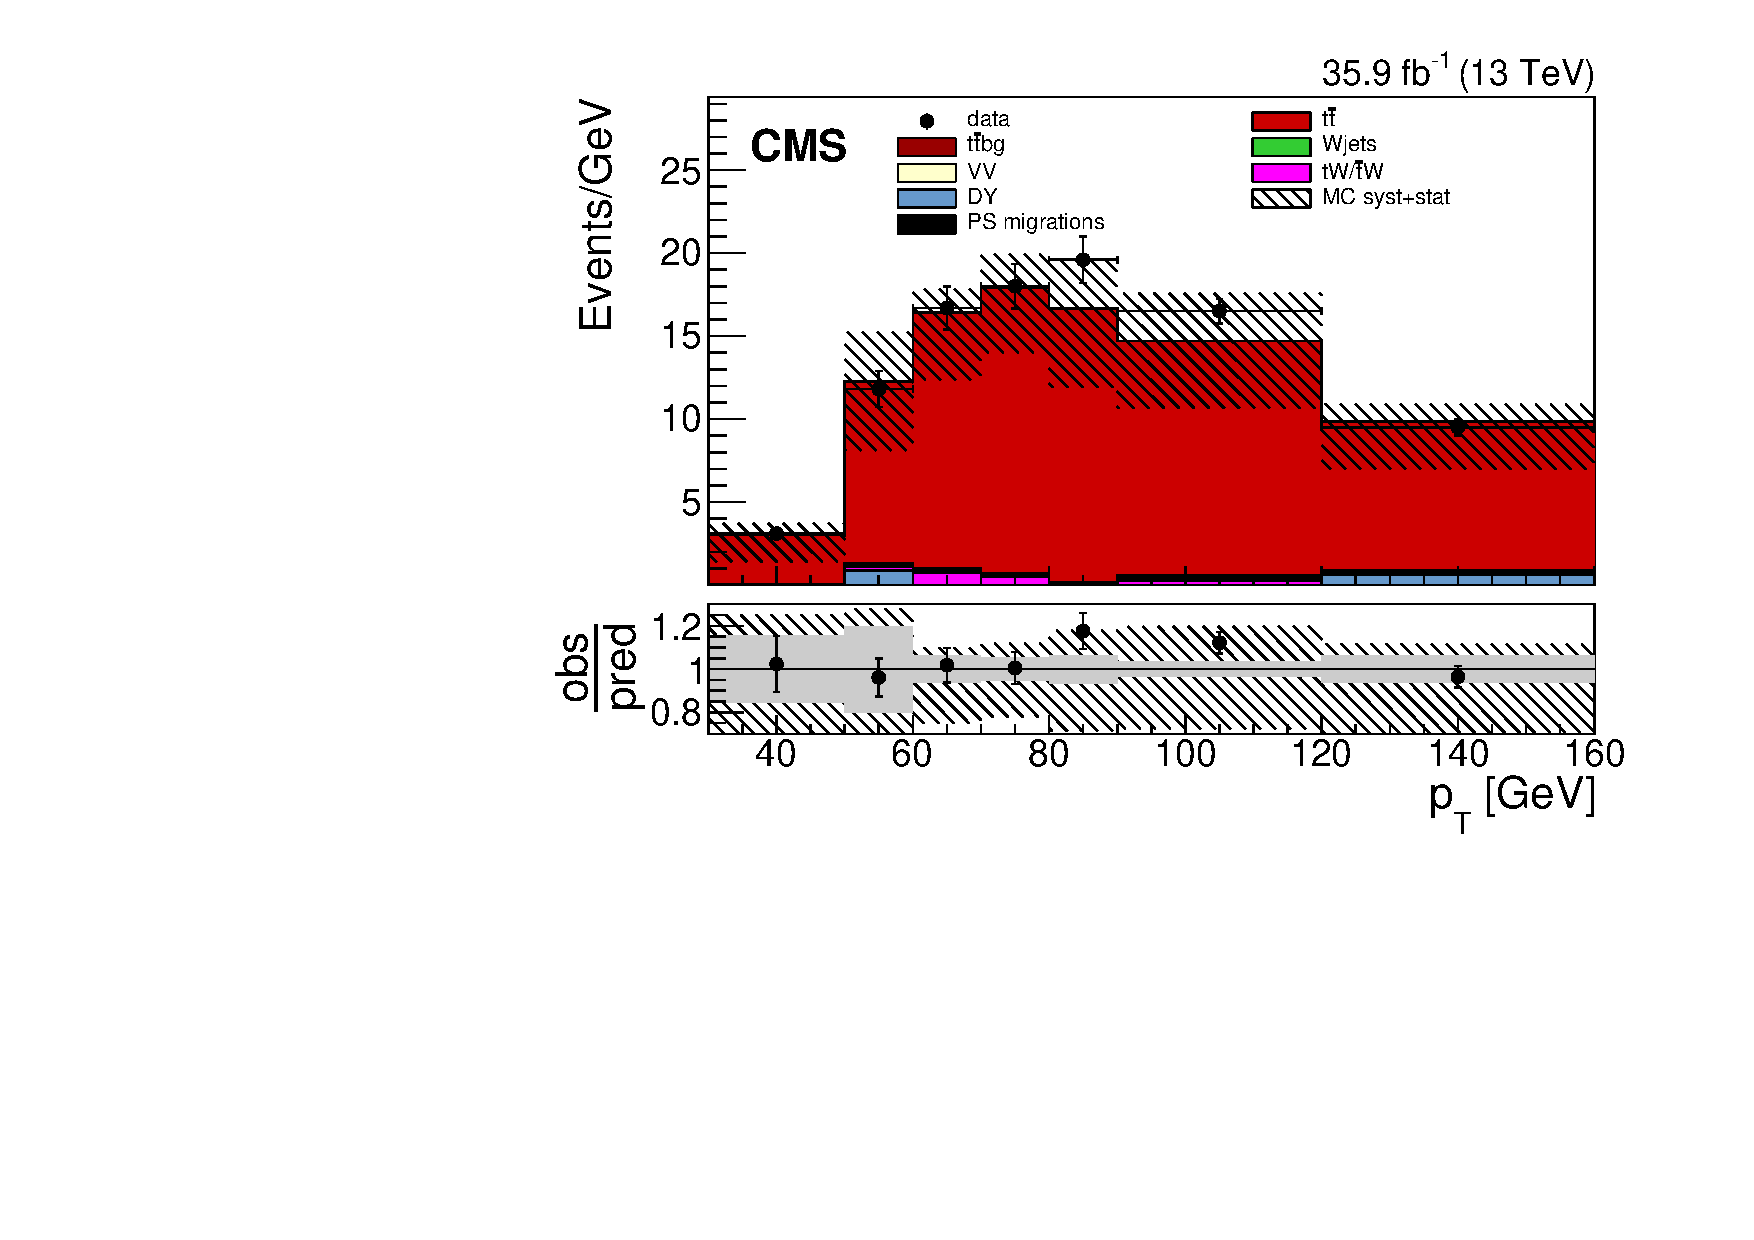
\includegraphics{CrossSection/Figures/ControlPlots/ee_sysnom/lead_jet_pt_2_1_b-jets_step_8.pdf}}\\
        
    \resizebox{0.4 \textwidth}{!}{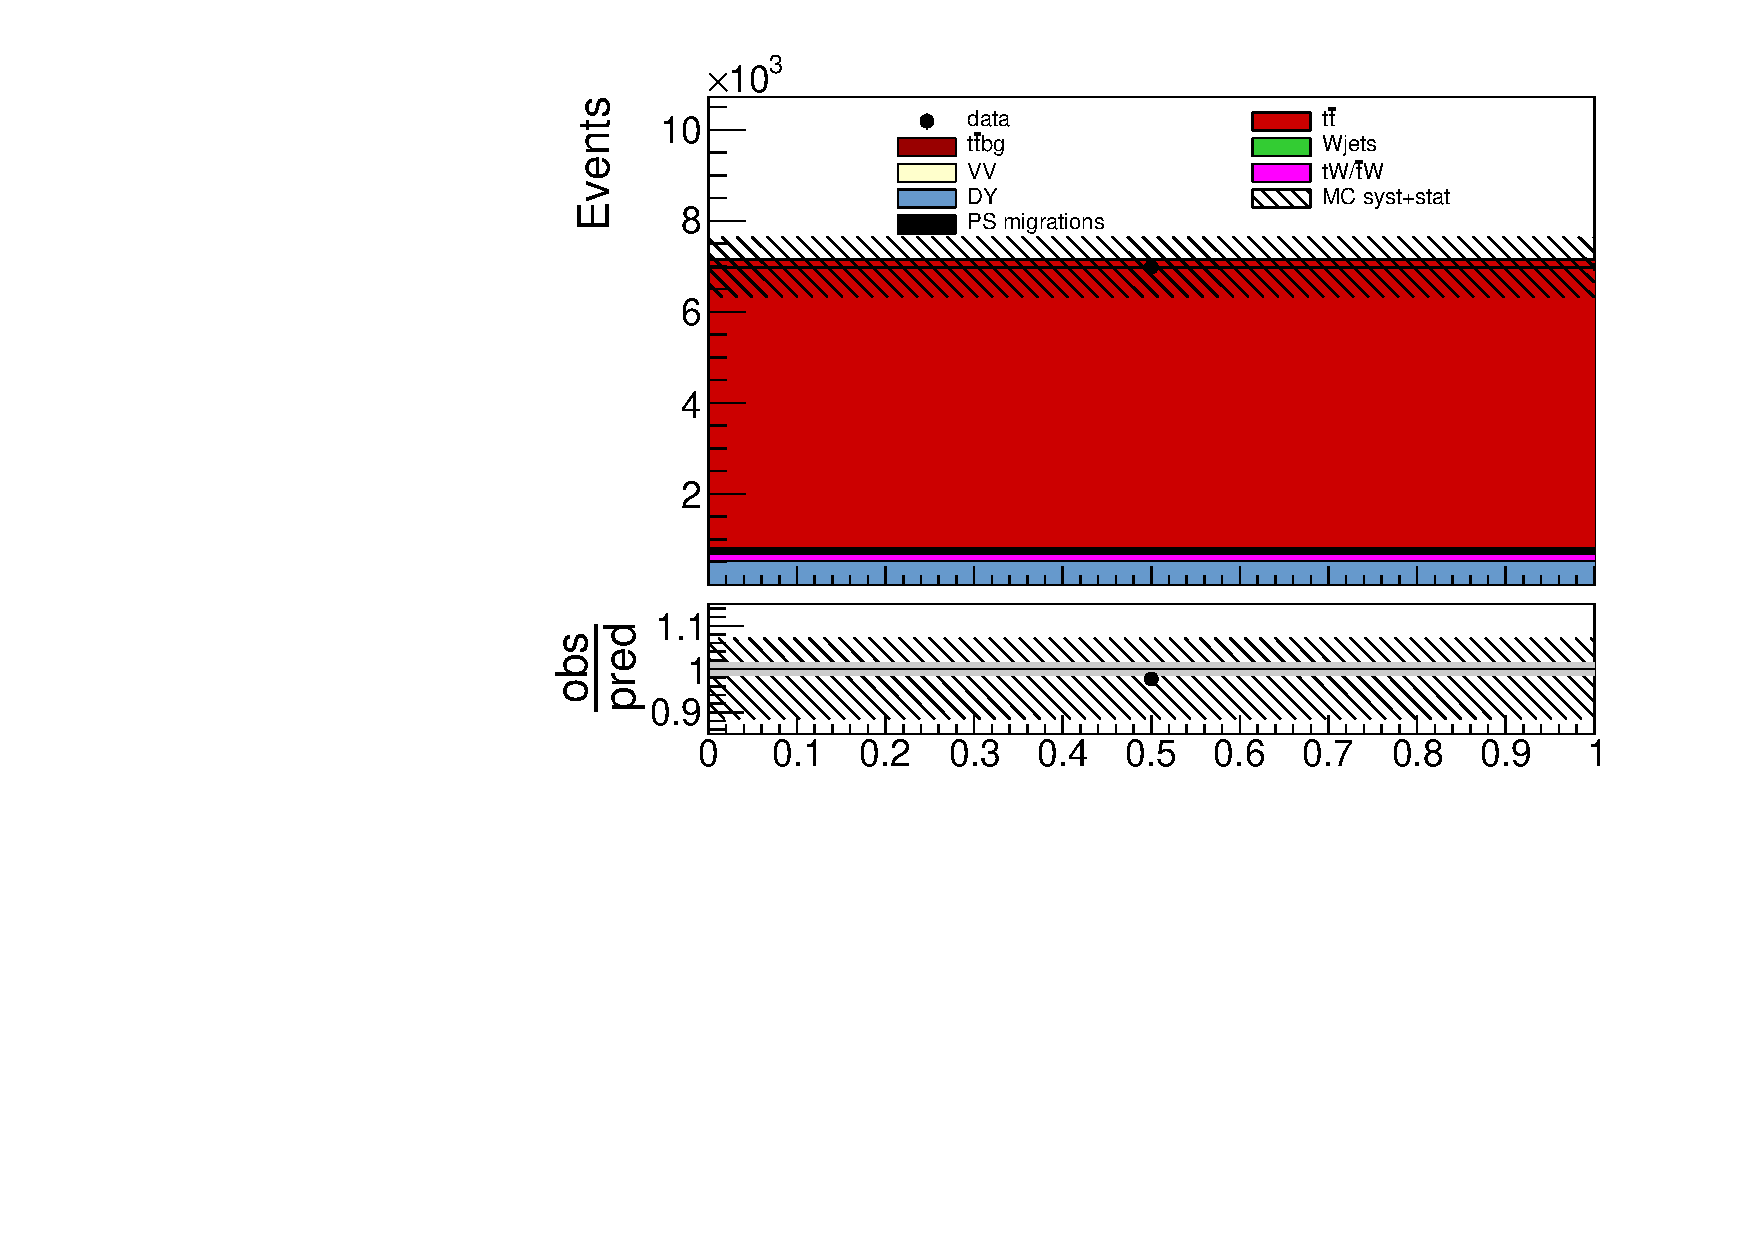
\includegraphics{CrossSection/Figures/ControlPlots/ee_sysnom/total_1_2_b-jets_step_8.pdf}}
    \resizebox{0.4 \textwidth}{!}{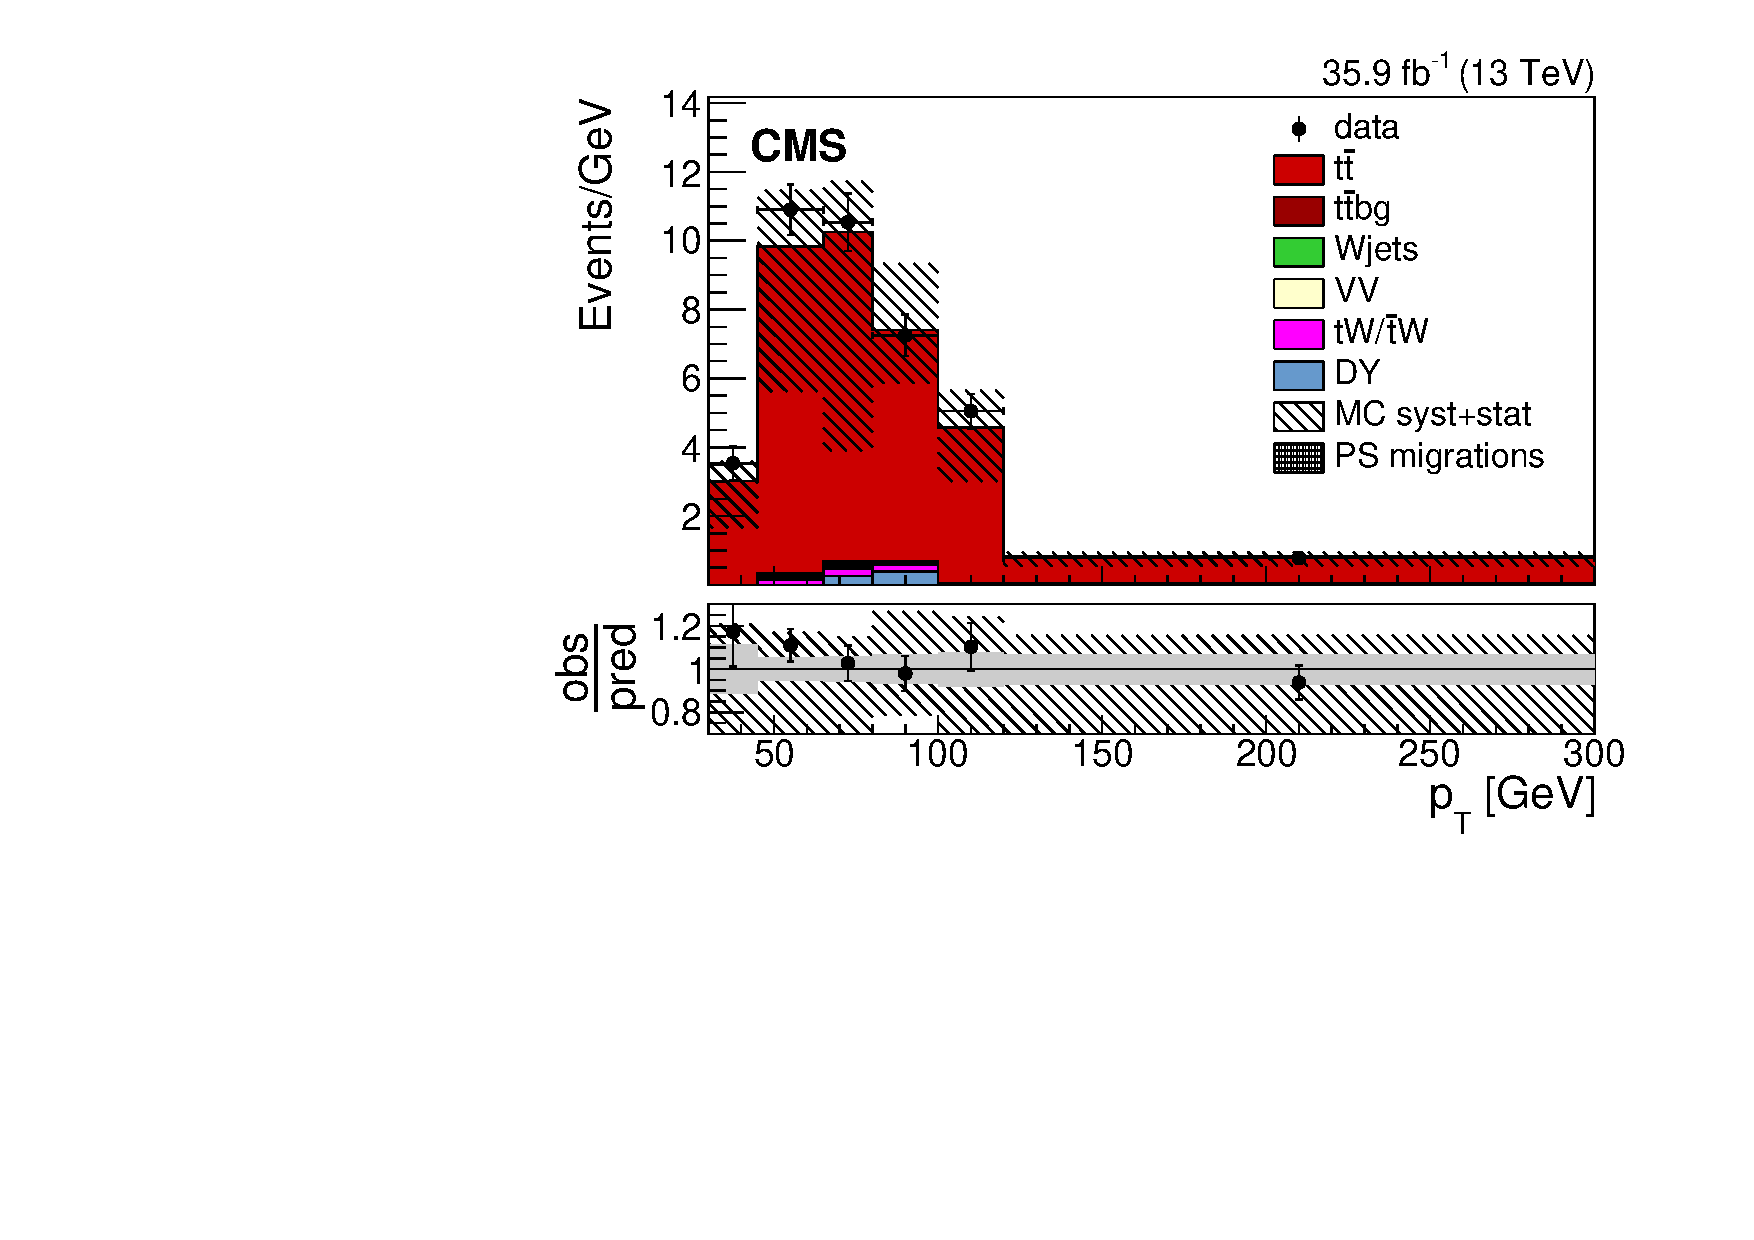
\includegraphics{CrossSection/Figures/ControlPlots/ee_sysnom/second_jet_pt_2_2_b-jets_step_8.pdf}}\\

    \resizebox{0.4 \textwidth}{!}{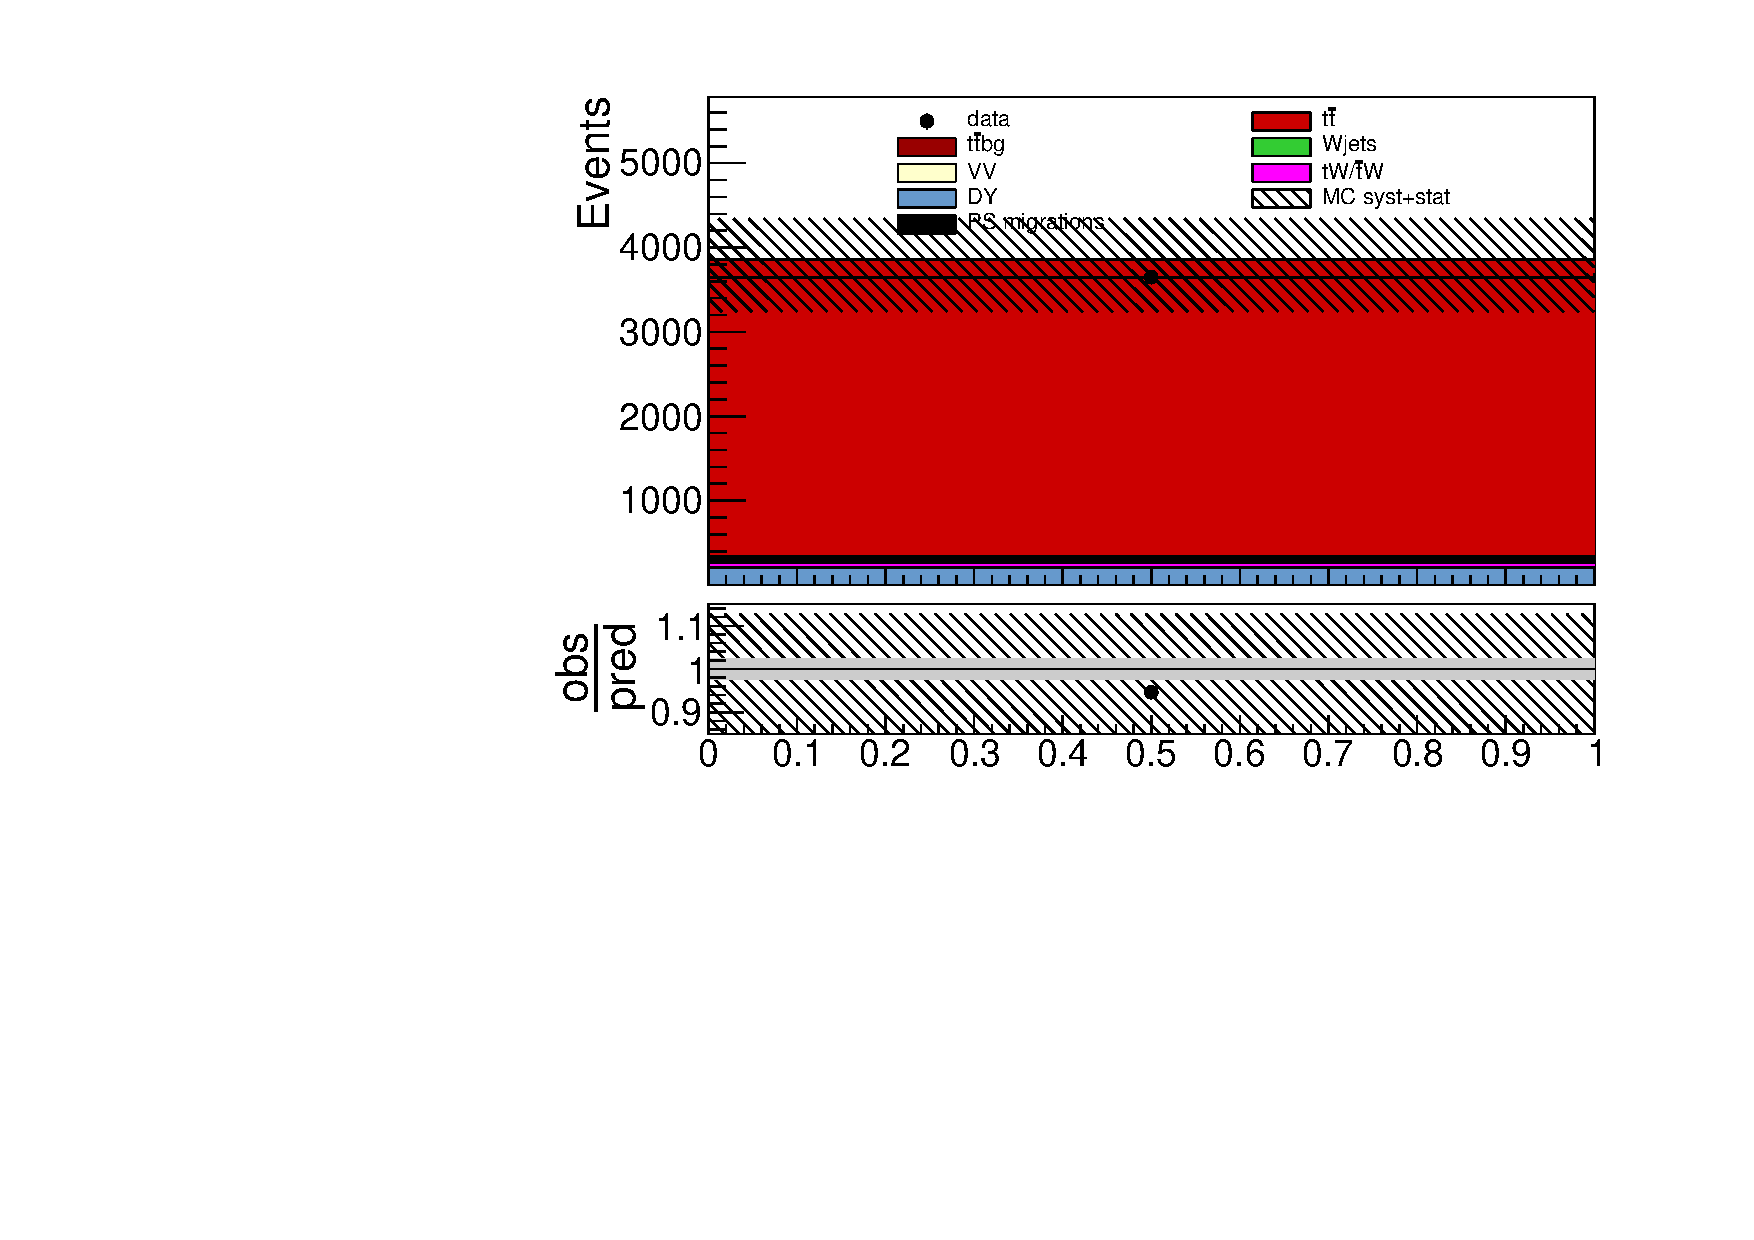
\includegraphics{CrossSection/Figures/ControlPlots/ee_sysnom/total_1_3_b-jets_step_8.pdf}}
    \resizebox{0.4 \textwidth}{!}{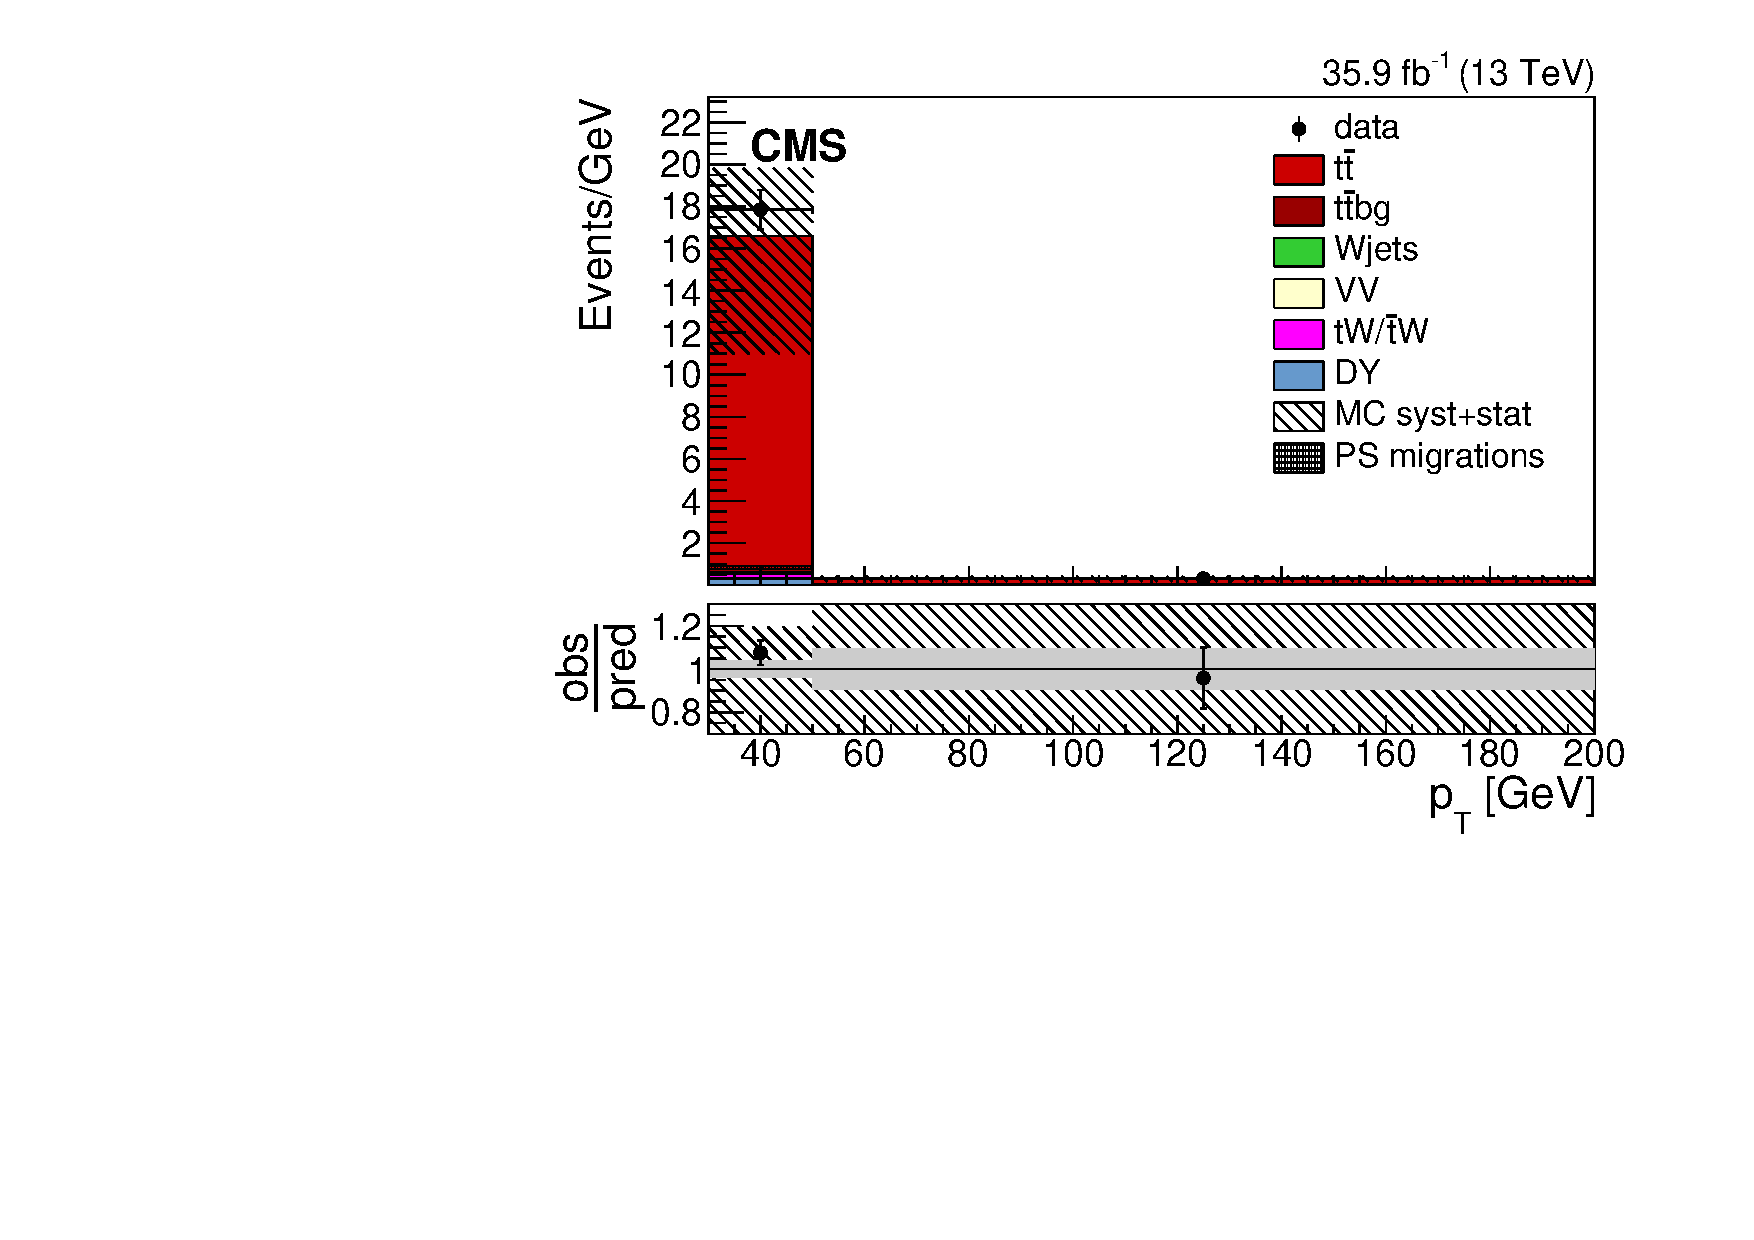
\includegraphics{CrossSection/Figures/ControlPlots/ee_sysnom/third_jet_pt_2_3_b-jets_step_8.pdf}} 
\caption{Template distributions for events in the \ee channel with one b-tagged jet (left column) or two b-tagged jets (right column). The distributions show the total event yield for zero (top) nd the trailing jet pt for one (second from top),
  two (second from bottom) or three or more (bottom) additional jets. 
  The hatched bands correspond to the total uncertainty on the predicted number of events. The ratios of the event yields in data and the sum of the
  predicted yields are shown at the bottom of each plot. Here, the solid
  gray band represents the contribution of the statistical uncertainty.  
       \label{fig:xsec_ee_inputdistr}}
  \end{center}
\end{figure}


    
\section{Definition of the $\chi^2$ Function}
\label{sec:xsec_stat}

A binned $\chi^2$ fit is used to extract the \ttbar cross section using the event categorisation described above. Beside the \ttbar cross section the efficiency to find a b tagged jets is also determined.
The number of expected events for signal and background is fitted to the number of measured events. The number of \ttbar events depends on the \ttbar cross section, which allows to extract the later from a fit of the former.
Additionally, the expected number of \ttbar events depends on the systematic uncertainties which are included as nuisance parameters. The normalization of the background processes is also included as a separate nuisance parameter for each of the separate background processes.

The nuisance parameters are fitted as well, but the phase space of each nuisance parameter is typically restricted according
to a priori assumptions based on external measurements. These assumptions are usually expressed as probability distributions also denoted as priors.
In case these probability distributions are not flat a so called penalty term is introduced to the fit to express the improbability to find such a value for this specific systematic uncertainty.

In order to perform the fit the following expression is minimised:

\begin{eqnarray}
   \chi^2  &=& \sum_{i} \frac{(n_i-\mu_i)^2}{\delta_{n_i}^2+ \delta_{\mu_i}^2} + \sum_{l} \pi(\omega_l) + \sum_{m} \pi(\lambda_m) \\
 \mathrm{where} \; \; \; \; \; \mu_i &=& s_i(\stt,\vec{\lambda}) + \sum_{l} b_{l,i}(\omega_l,\vec{\lambda}).
\label{eq:xsec_chisqfunct}
\end{eqnarray}

Here the index $i$ represents a single bin, while $n_i$ is the number of measured events in data. The symbol $\mu_i$ represents the number
of expected events in simulation. The statistical uncertainties on the measured and expected number of events is introduced as $\delta_{n_i}$ and $\delta_{\mu_i}$ respectively. The terms $\omega_l$ and $\lambda_m$
denote the nuisance parameters, with the $\pi$ standing for the penalty term related to a Gaussian prior.
The second equation breaks down the expected number of events $\mu_i$ per bin $i$ into the number of signal events $s_i$ depending on the \ttbar cross section $\stt$ and all relevant nuisance parameters $\vec{\lambda}$ and the number of
background events  $b_{l,i}$ for each background process $l$ also depending on the nuisance parameters and the normalisation of the respective background process $\omega_l$.

A unit normal distribution is chosen as probability density function for nuisance parameters with gaussian priors. Other nuisance parameters have a uniform prior and do not contribute any penalty terms. 
Since a uniform probability distribution has either a flat value or a value of zero no special term for the nuisance parameter is prefered (unless it is forbidden), consequently no punishment term is needed. Parts of the phase space where the probability density is zero are explicitly forbidden in the fit.

As described above the number of expected events for a background process also depends on the nuisance parameters. Especially nuisance paramters related to experimental systematic uncertainties affect the signal as well as the background processes. For example the uncertainty on the muon reconstruction efficiency affects all events containing a muon (background as well as signal), while an uncertainties related to theory uncertainties usually only applies to the \ttbar signal. The details can be found in Section \ref{sec:syst_uncert}.

The number of background events can then be decomposed to :

\begin{equation}
b_{l,i}(\omega_l,\vec{\lambda}) = b_{l,i}^{MC}(\vec{\lambda}) \cdot (1 + \omega_l).
\label{eq:nbli}
\end{equation}

Here, $b_{l,i}^{MC}$ denotes the expected number of events from the simulation of the respective background process and $\omega_l$ denotes the normalization. The uncertainty on the normalization of a specific process is propagated
by a variation of the respective $\omega_l$.
The number of background events in simulation depends on the nuisance parameters $\vec{\lambda}$.

Following the description in Section \ref{sec:xsec_templates}  the number of signal events is further devided according to the number of b-tagged jets.
The number of events in the categories for events with zero or more than two b-tagged jets $s_{0,b}$, for events with exactly one $s_{1,b}$ and for events with exactly two b-tagged jets $s_{2,b}$ are expressed as follows:

\begin{eqnarray}
s_{0,b}  &=& \mathcal{L}_{\rm int}\sttvis \epsilon_{e\mu} \cdot (1-2\epsilon_b(1-C_b\epsilon_b)-C_b\epsilon_b^2) \\
s_{1,b}  &=& \mathcal{L}_{\rm int} \sttvis \epsilon_{ll} \cdot 2 \epsilon_b(1-C_b\epsilon_b) \\
s_{2,b}  &=& \mathcal{L}_{\rm int} \sttvis \epsilon_{ll} \cdot   \epsilon_b^2 C_b.
\label{eq:xsec_nb}.
\end{eqnarray}
Only events in the \emu channel contribute to category $s_{0,b}$.
Here, $\mathcal{L}_{\rm int}$ denotes the integrated luminosity, $\sttvis$ the visible \ttbar cross section and $\epsilon_{ll}$ the efficiency of the dilepton selection.
The b-tag efficiency $\epsilon_b$ is the probability to reconstruct a b-tagged jet in a \ttbar event. It includes the efficiency of the b-tagging algorithm, the geometrical acceptance of the kinematic cuts on the b-jet ($\pt > 30\; \GeV, |\eta|<2.4$) and the probability of a light jet to be b-tagged. In general the contribution of the geometrical acceptance and the mis-tag rate is comparatively low (see Section \ref{sec:SimReco_BjetReco} for the mistag rate).
It is assumed that the two b-jets can be identified independently of each other. Remaining correlations between the b tagging efficiencies for both jets are described by the parameter $C_b$. These correlations can also be expressed in terms of the events measured in the separate categories: $C_b=4s_{ll}s_{2,b}/(s_{1,b}+2s_{2,b})^2$ where $s_{ll}$ is the total number of selected \ttbar events. 

The values for $\epsilon_{ll}$ and $s_{i}$ are obtained from simulation and depend on the nuisance parameters $\vec{\lambda}$. Any constraint of these parameters also constrains the related nuisance parameters.

The visible cross section corresponds to the cross section in the fiducial phase space as defined in Section \ref{sec:xsec_sel}. The requirement to select one b-tagged jet in the same flavor channels is absorbed into $\epsilon_{\mathrm{ee}}$ or $\epsilon_{\mu\mu}$ respectively.
In the fiducial phase space all systematic uncertainties and the related nuisance parameters can be constrained.

The dependence of the template distributions on the nuisance parameters is modeled with a second order polynomial which is constructed using the nominal and the two systematically varied values of each nuisance parameter $\lambda_m=0, 1, -1$.
The variation of the respective template distributions in each bin depends on the value of $\lambda$, with $\lambda = \pm 1$ corresponding to a $ \pm 1 \cdot \sigma$ variation. If multiple templates distributions are affected by one uncertainty or nuisance parameter all of them are varied coherently.
The template distributions are then added up to the expected number of events in each bin, as shown in Equation \ref{eq:xsec_chisqfunct}. The expected number of events consequently mirrors the dependence of the template distributions on the nuisance parameters.
Some nuisance parameters are based on a one-sided variation so only one systematically varied value exists. In these cases the dependence of the template distributions on the nuisance parameters is modeled by a linear function.

The MINUIT~\cite{James:1975dr} algorithm is used to minimize the  $\chi^2$ term (see \ref{eq:xsec_chisqfunct} ) as function of the free fit parameters $\stt$, $\vec{\omega}$
and $\vec{\lambda}$. 

The nuisance parameters are apriori assumed to be uncorrelated, but the simultaneous fit takes possible correlations into account. Parameters having a similar effect on the fitted parameters will be correlated by the fit.
An example for this are the nuisance parameters for the uncertainties on the lepton efficiencies, which are already discussed in Section \ref{sec:xsec_templates}. Both lepton efficiencies affect the number of events and the overall selection efficiency in a similar way in the \emu channel leading to a strong correlation between these two parameters.

The choice of event categories and the parametrization of the $\chi^2$ function should allow a constraint of several relevant systematic uncertainties of the \ttbar cross section.
Uncertainties related to jets and especially b jets should be reduced after the fit. As shown below (see Section \ref{sec:syst_uncert}) this includes a wide array of different systematic uncertainties
from the uncertainty on the b jet identification to the uncertainty on the scale for final state radiation in the parton shower. The uncertainties on the lepton efficiencies are expected to be constraint as well, due to the separation into the three decay channels.
Uncertainties that change the normalization of all processes like the uncertainty on the trigger efficiency or the luminosity are not expected to be constrained by the fit.


\section{Extrapolation from the visible to the Full Phase Space}
\label{sec:xsec_extraction}

The previous section only referred to the visible cross section in the fiducial phase space. In order to extrapolate that result to the full phase space the acceptance
is estimated.
In contrast to the measurement of the visible cross section not all systematic uncertainties can be constrained for the extrapolation of the cross section from the fiducial to the full phase space.
Similar to the cross section itself, some of the uncertainties need to be extrapolated and can not to constrained for the extrapolation.

The acceptance is defined by the kinematic selection requirements on the leptons. As detailed in Section \ref{sec:xsec_sel} the two leptons are required to be part of the $t \rightarrow W b$ decay. They are further required to be within $|\eta|< 2.4$ with the 
leading lepton having $\pt > 25 \; \GeV$ and the trailing lepton $\pt > 20 \; \GeV$. The invariant mass of the dilepton system is required to be $\mll > 20 \; \GeV$. 

The acceptance can be introduced by replacing the efficiency of the dilepton selection as follows:

\begin{equation}
\epsilon_{ll} = A_{ll} \epsilon_{ll}.
\label{eq:epsacc}
\end{equation}

Here $A_{ll}$ is the acceptance and $\epsilon_{ll}$ is the efficiency in the visible phase space, both depending on the nuisance parameters $\vec{\lambda}$.
Correspondinly the visible cross section can be extrapolated to the full cross section by dividing it by the acceptance: $\sttbar = \sttvis / A_{ll}$, again both the visible cross section and the 
acceptance depend on the nuisance parameters.

The values for the nuisance parameters that are determined in the fit of the visible cross section are propagated to the acceptance, including the correlations brtween the nuisance parameters. 
Similarly the constraints for most of the nuisance parameters are applied to the calculation of the uncertainty of the acceptance.
Some of the nuisance parameters should only be constrained in the visual phase space and should be left unconstrained in the extrapolation.
Espacially uncertainties that affect the behaviour of the prediction in the visible phase space have to be extrapolated.

The extrapolation of an uncertainty takes the fitted value of each relevant nuisance parameter as central value. Then the change of acceptance for the explicit $\pm 1 \sigma$ variation is considered as the $\pm 1 \sigma$ variation on the acceptance. These additional uncertainties are then added to the uncertainty of the cross section extracted to the full phase spacefor each relevant nuisance parameter. These additional uncertainties are treated as uncorrelated and are added up in quadrature. This procedure can lead to asymmetric variations, even for originally symmetric variations in case the fitted value of the nuisance parameter is not the original central value.

The following uncertainties are extrapolated:
The uncertainty on the PDF, the top \pt uncertainty, the uncertainty on the matrix element scale and the uncertainties on the parton shower tune, the initial and final state radiation scales.



